\ifcase0  % choose 0=slides, 1=article, 2=refart
	 \documentclass[ignorenonframetext,12pt]{beamer}
	 \geometry{paper=a6paper,landscape}
\or\documentclass[a4paper,11pt]{article}
	 \usepackage{url,beamerarticle}
\or\documentclass[a4paper,11pt]{refart}
	 \let\example\relax
	 \usepackage{url,beamerarticle}
\fi

\ifcase0  % choose a theme like these
%\usetheme{Montpellier}% I recommend
	 \usetheme{default}% I recommend
\or\usetheme{Singapore}
\or\usetheme{Szeged}
\or\usetheme{Boadilla}
\or\usetheme{Pittsburgh}
\or\usetheme{Madrid}
\or\usetheme{Warsaw} % common choice, but often poor
\fi

\usepackage[utf8]{inputenc}%para acentos en español
\usepackage{graphicx,pgfplots,parskip}
\usepackage{siunitx}
\usepackage{tikz}
\usepackage{tikz-cd}
\usetikzlibrary{tikzmark,fit}
\graphicspath{{media/}}
\usepackage{xcolor}
\usepackage[percent]{overpic}

\title[CAE2020]{Implementation of a Polyphase Filter Bank Channelizer on a Zynq FPGA}
\vspace{1cm}
\subtitle{{\color[rgb]{0.00,0.21,0.47}Congreso Argentino de Electrónica (CAE2020)\\ Buenos Aires - Argentina}}
\author[\texttt{@horacio\_arnaldi}]{Horacio Arnaldi \\ \texttt{{\href{mailto:arnaldi@cab.cnea.gov.ar}{arnaldi@cab.cnea.gov.ar}}}}
%\institute[LabDPR - CAB - IB]{Laboratorio Detección de Partículas y Radiación \\ Centro Atómico Bariloche - Instituto Balseiro}
%%\date{\today}
%\date{}
%\title[Proyecto LAGO]{Las electrónicas actuales de LAGO}
%\subtitle{Escuela Politécnica Nacional \\ Quito, Ecuador}
%\author[\texttt{@horacio\_arnaldi}]{Ing. Horacio Arnaldi \\ \texttt{{\href{mailto:arnaldi@cab.cnea.gov.ar}{arnaldi@cab.cnea.gov.ar}}}}
\institute[LabDPR - CAB - IB]{Laboratorio Detección de Partículas y Radiación \\ Centro Atómico Bariloche - Instituto Balseiro}
%\date{\today}
\date{}

%\title{Implementation of a Polyphase Filter Bank Channelizer on a Zynq FPGA}
%\subtitle{\alert{Charla de avance}}
%\author{Horacio Arnaldi\\
%\vspace{0.4cm}
%Director: Dr. Ing. Damián Dellavale\\
%Co-Director: Dr. Ing. José Lipovetzky\\
%\vspace{0.6cm}
%Instituto Balseiro}
%\date{12 de Diciembre, 2019}

\begin{document}

\begin{frame}
				\maketitle
\end{frame}

\begin{abstract}
				This abstract, being outside the frame environment, does not appear in
				the presentation.  Your outline will be the basis for a couple of
				sentences of talk for each of the following questions:
				\begin{itemize}
								\item What was done?
								\item Why do it?
								\item What were the results?
								\item What do the results mean in theory and/or practise?
								\item What is the reader's benefit?
								\item How can the readers use this information for themselves? 
				\end{itemize}
\end{abstract}

%\begin{frame}{Outline}
%				\tableofcontents
%\end{frame}

%------------------------------------------------------------------------------
\section{Motivación}
\begin{frame}{Motivación}
				\begin{columns}
								\begin{column}{0.5\textwidth}
												\begin{itemize}
																\item Aplicación (CMB, Dark Mater, TMUX)
																\item Detectores (MKID, QUBIC)
																\item Electrónica (FPGA, GPU, CPU, etc)
												\end{itemize}
								\end{column}
								\begin{column}{0.5\textwidth}
												\only<1>{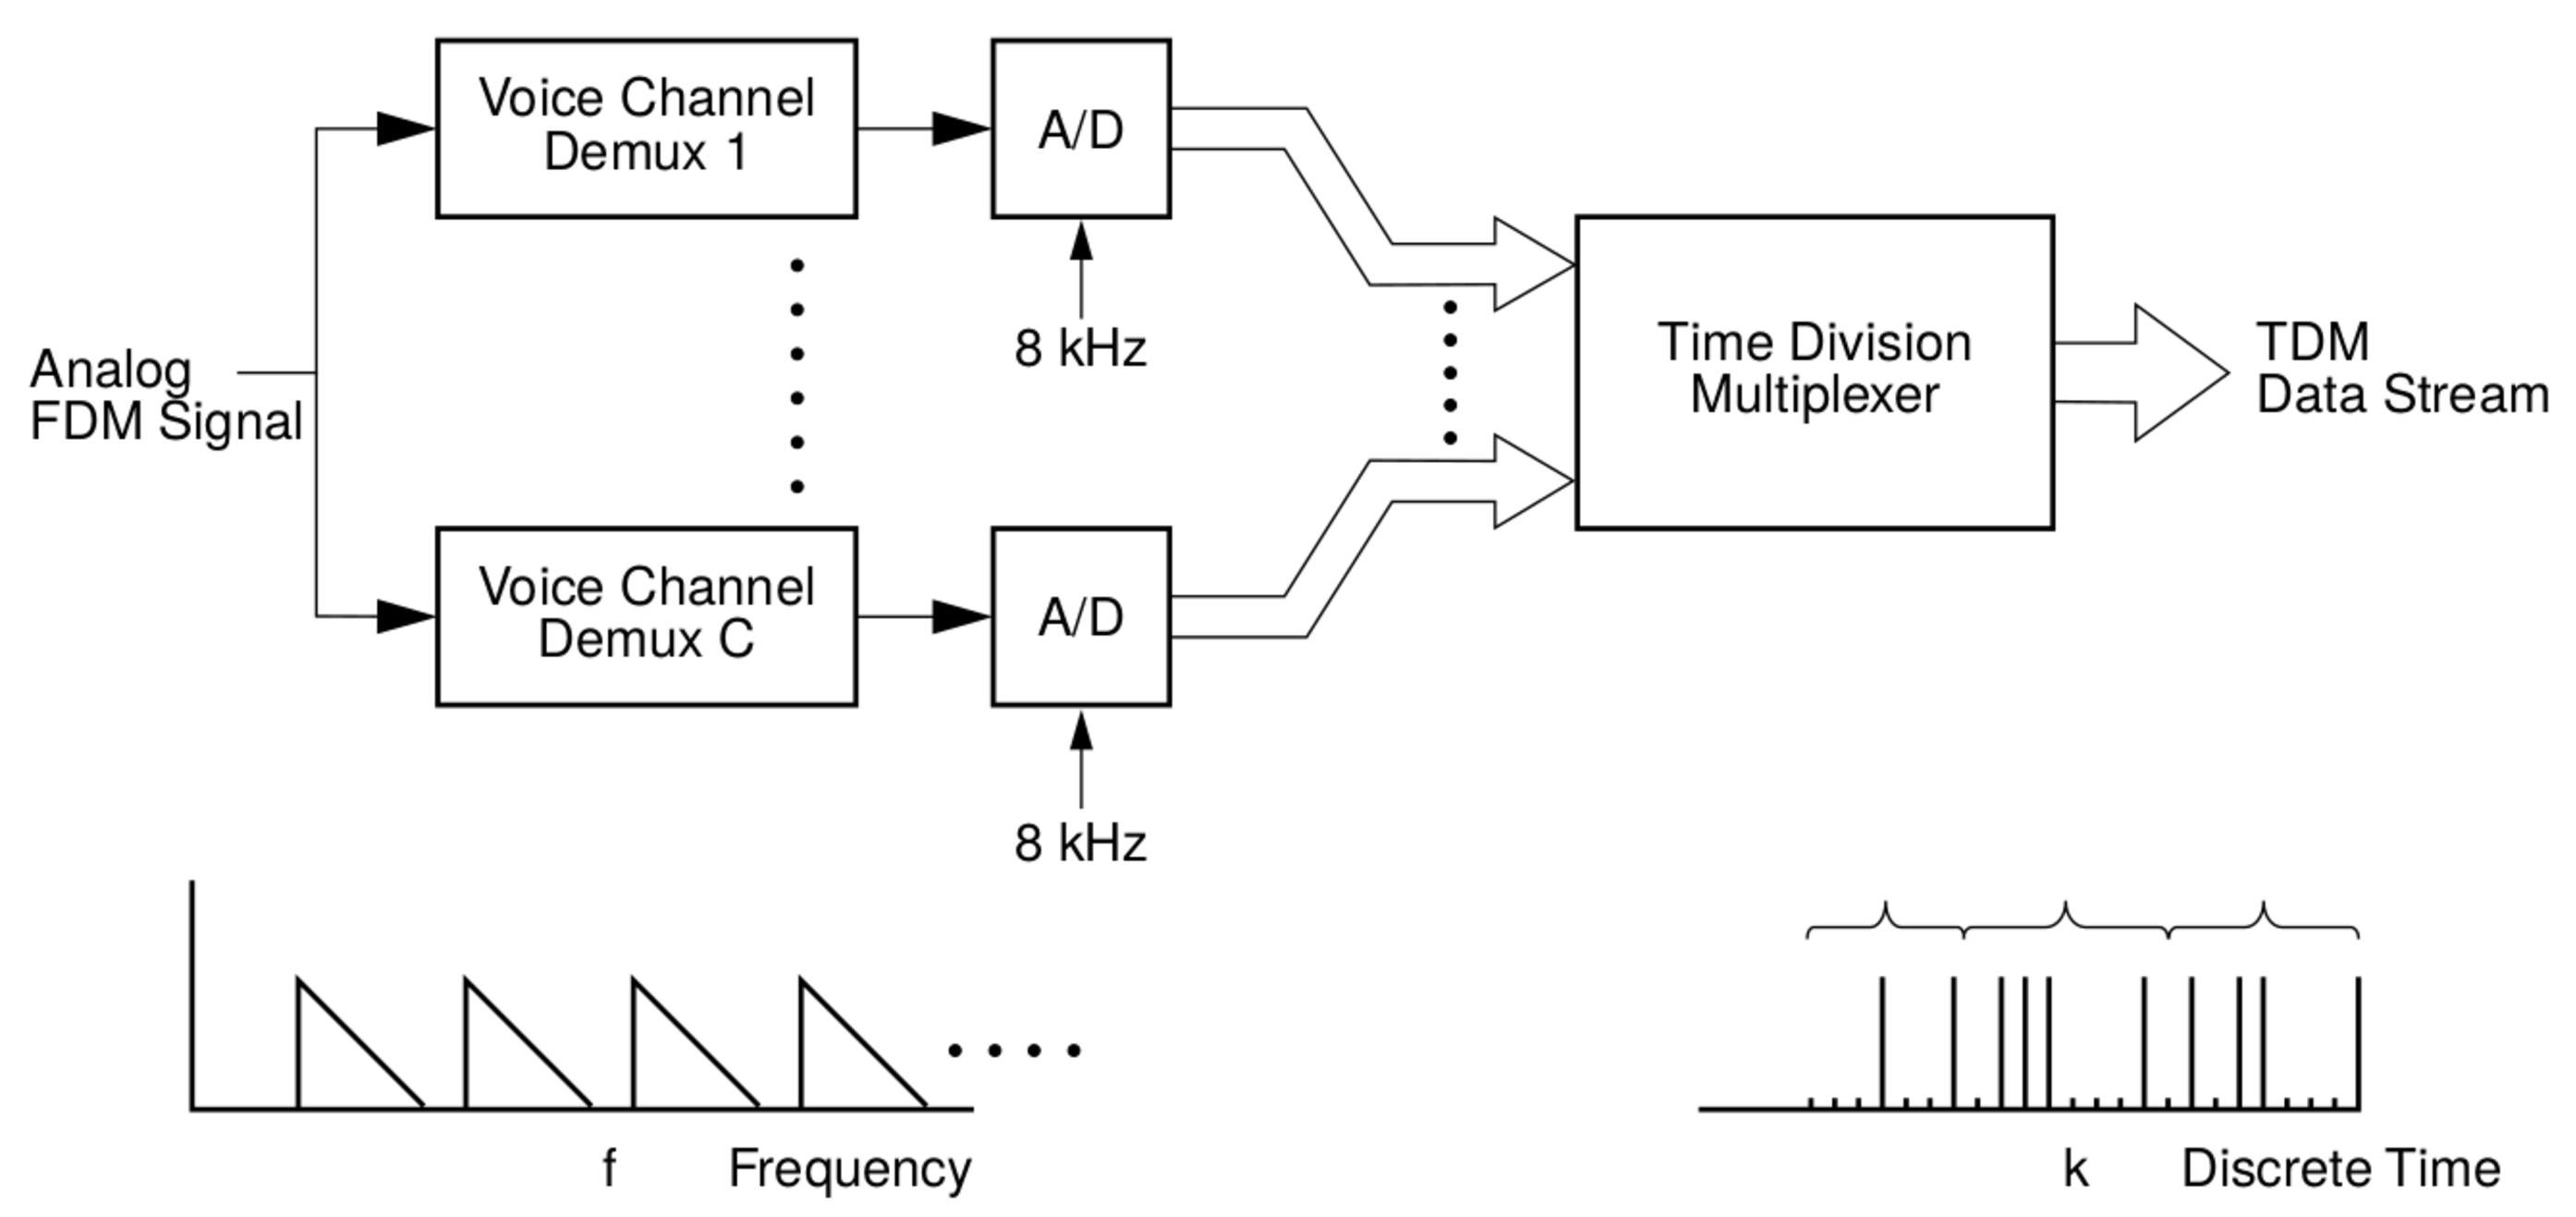
\includegraphics[width=1.1\textwidth]{tmux_usos}}
								\end{column}
				\end{columns}
												\only<1>{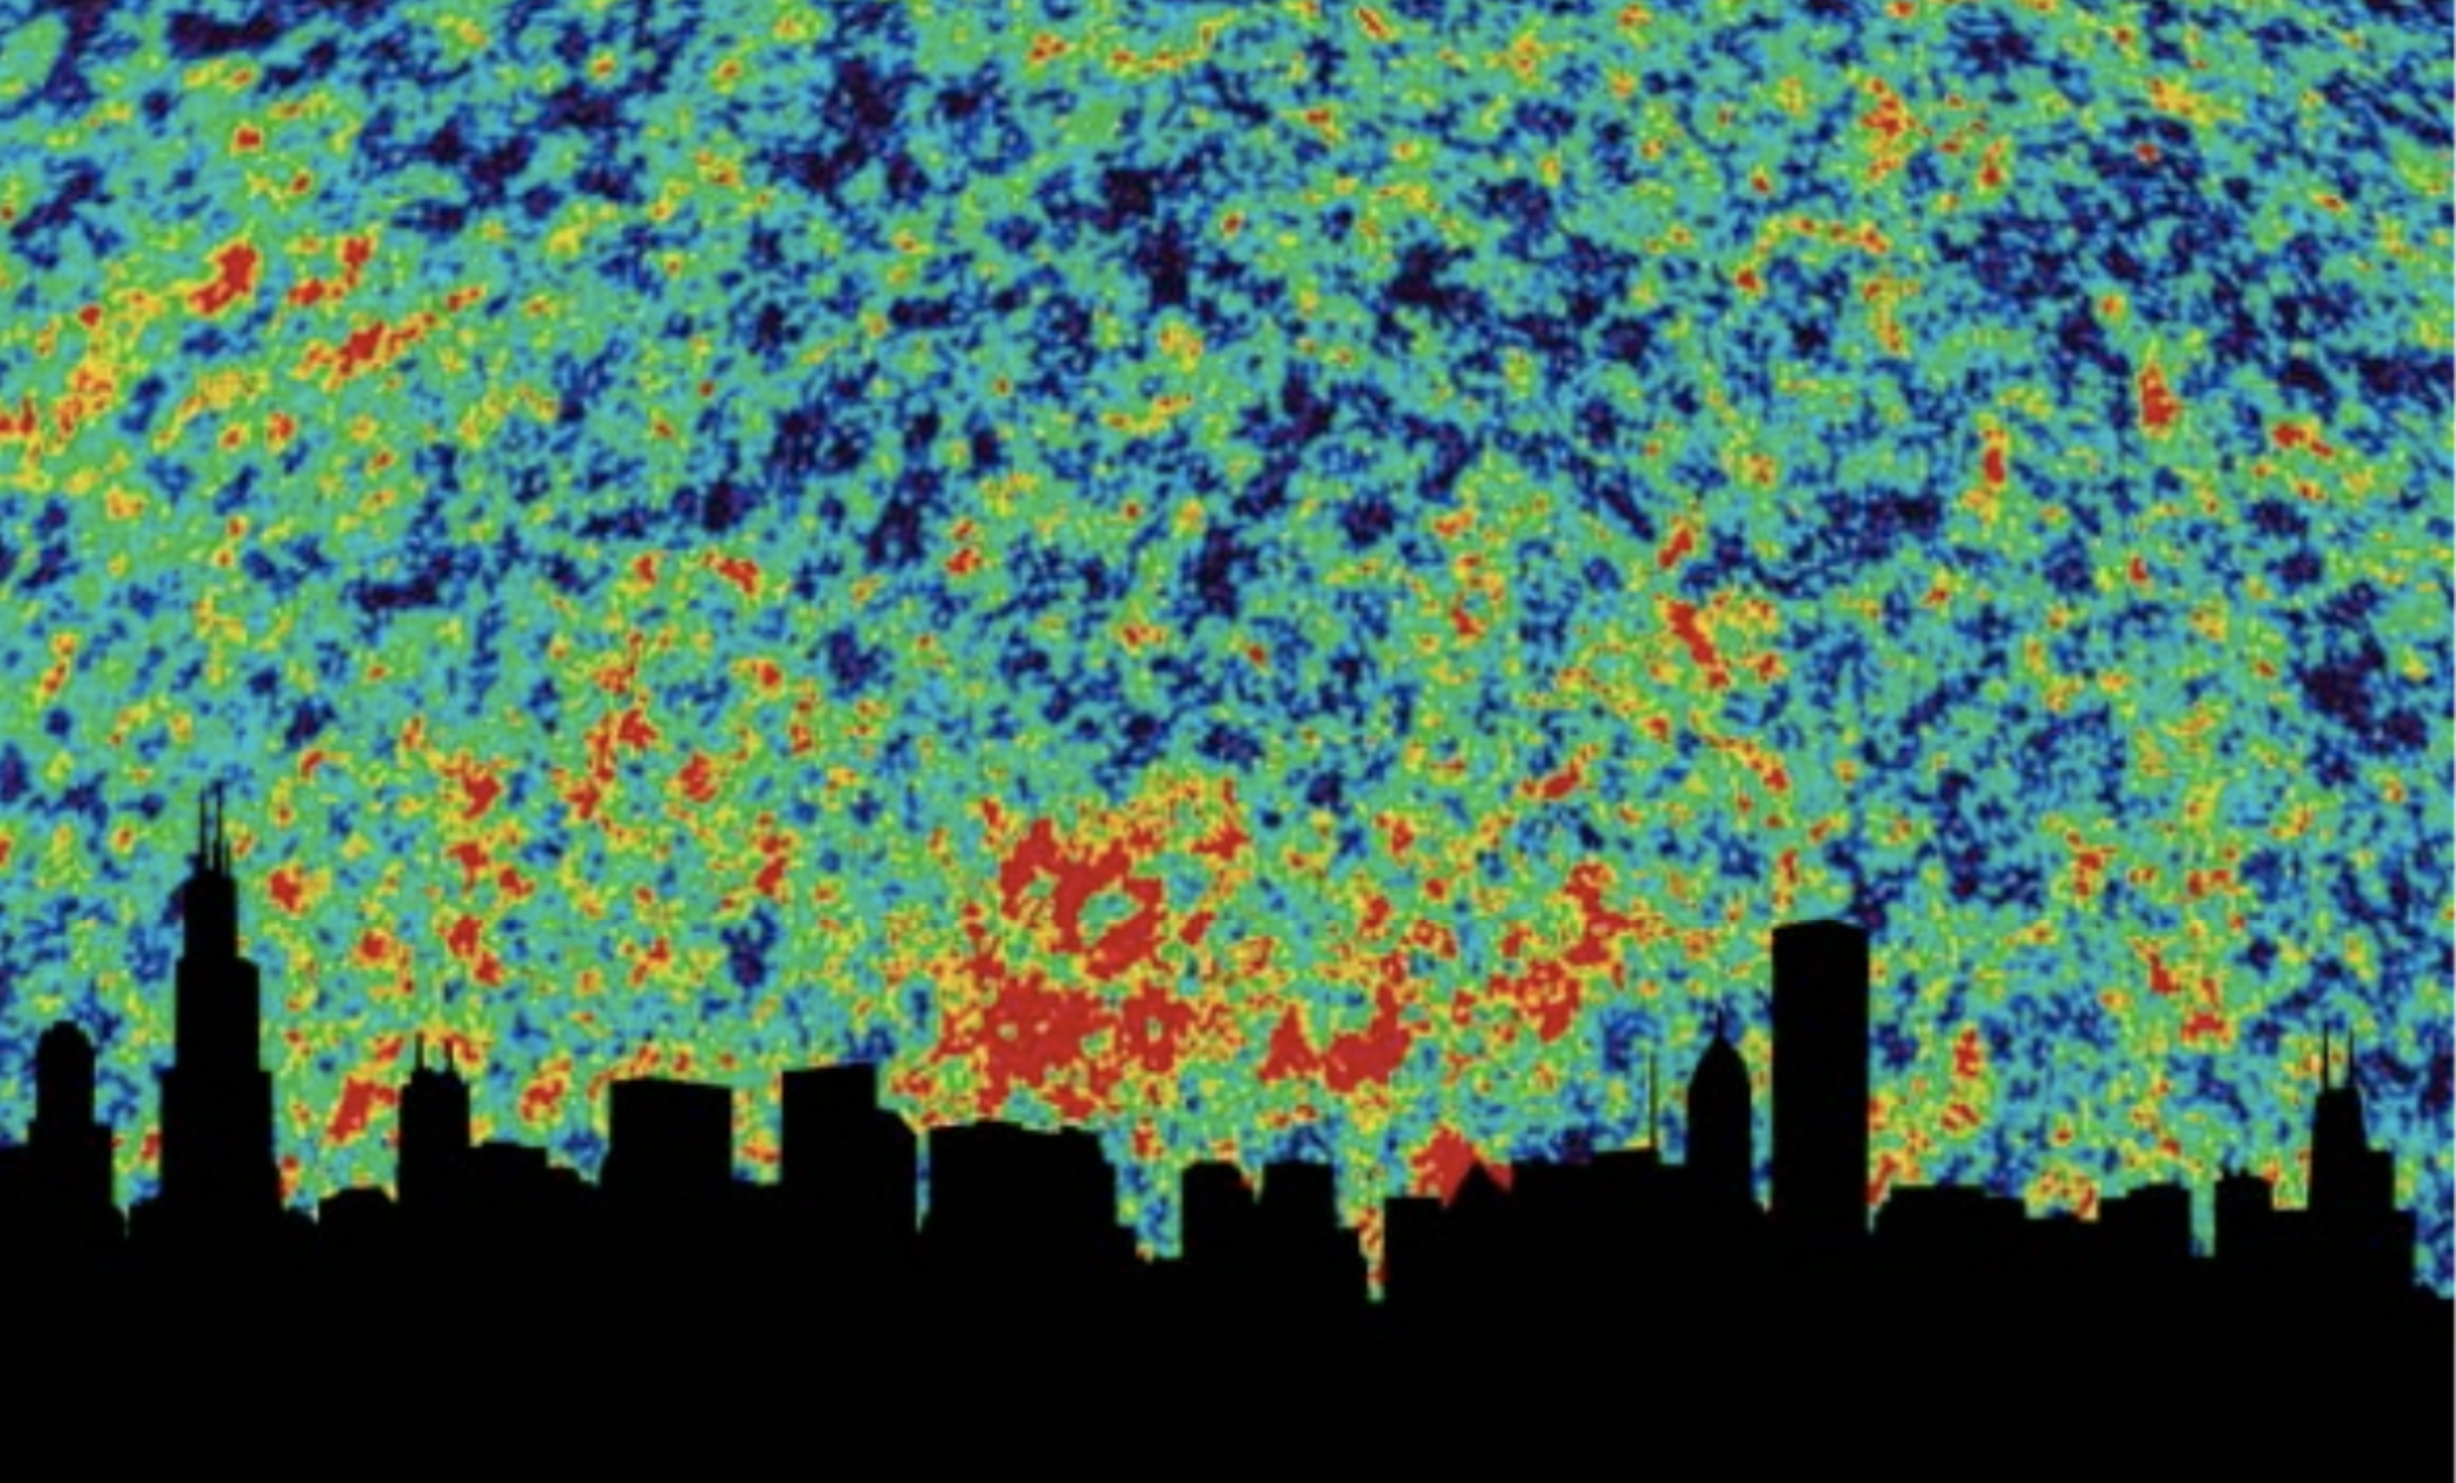
\includegraphics[width=0.45\textwidth]{motivacion1}}
												\only<1>{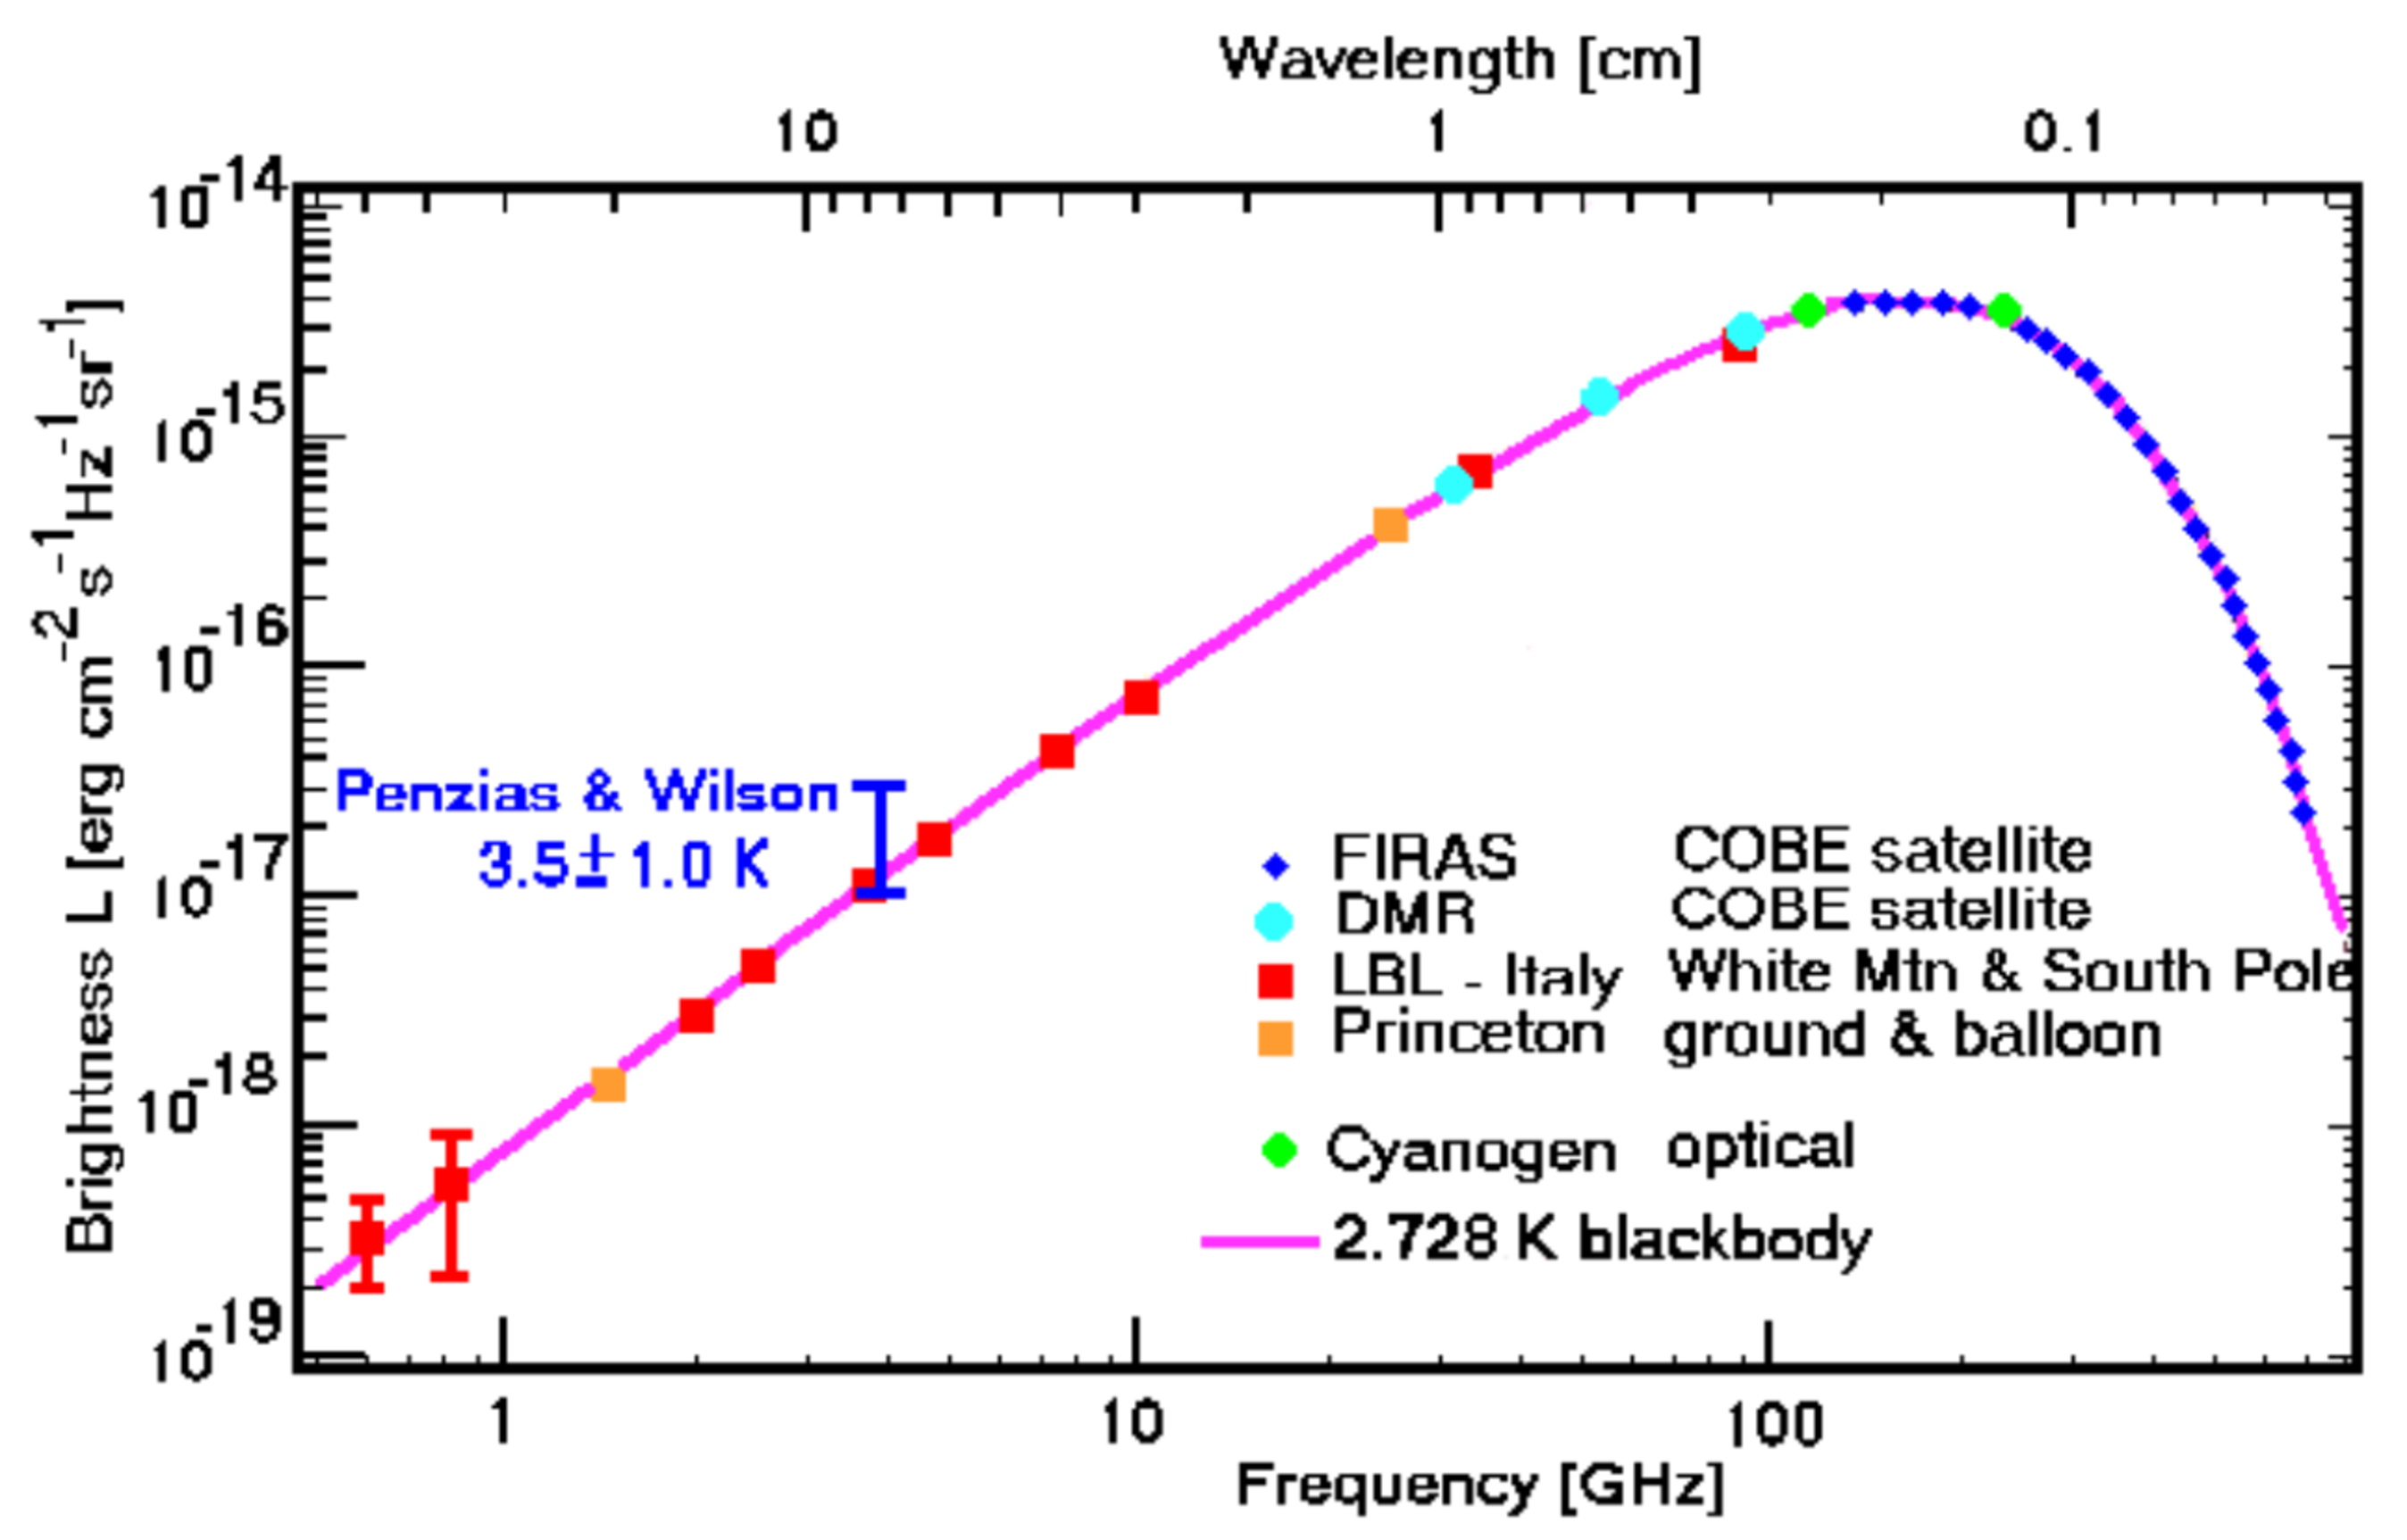
\includegraphics[width=0.45\textwidth]{motivacion4}}
												\only<2>{
\includegraphics[width=0.3\textwidth]{qubic1}}
												\only<2>{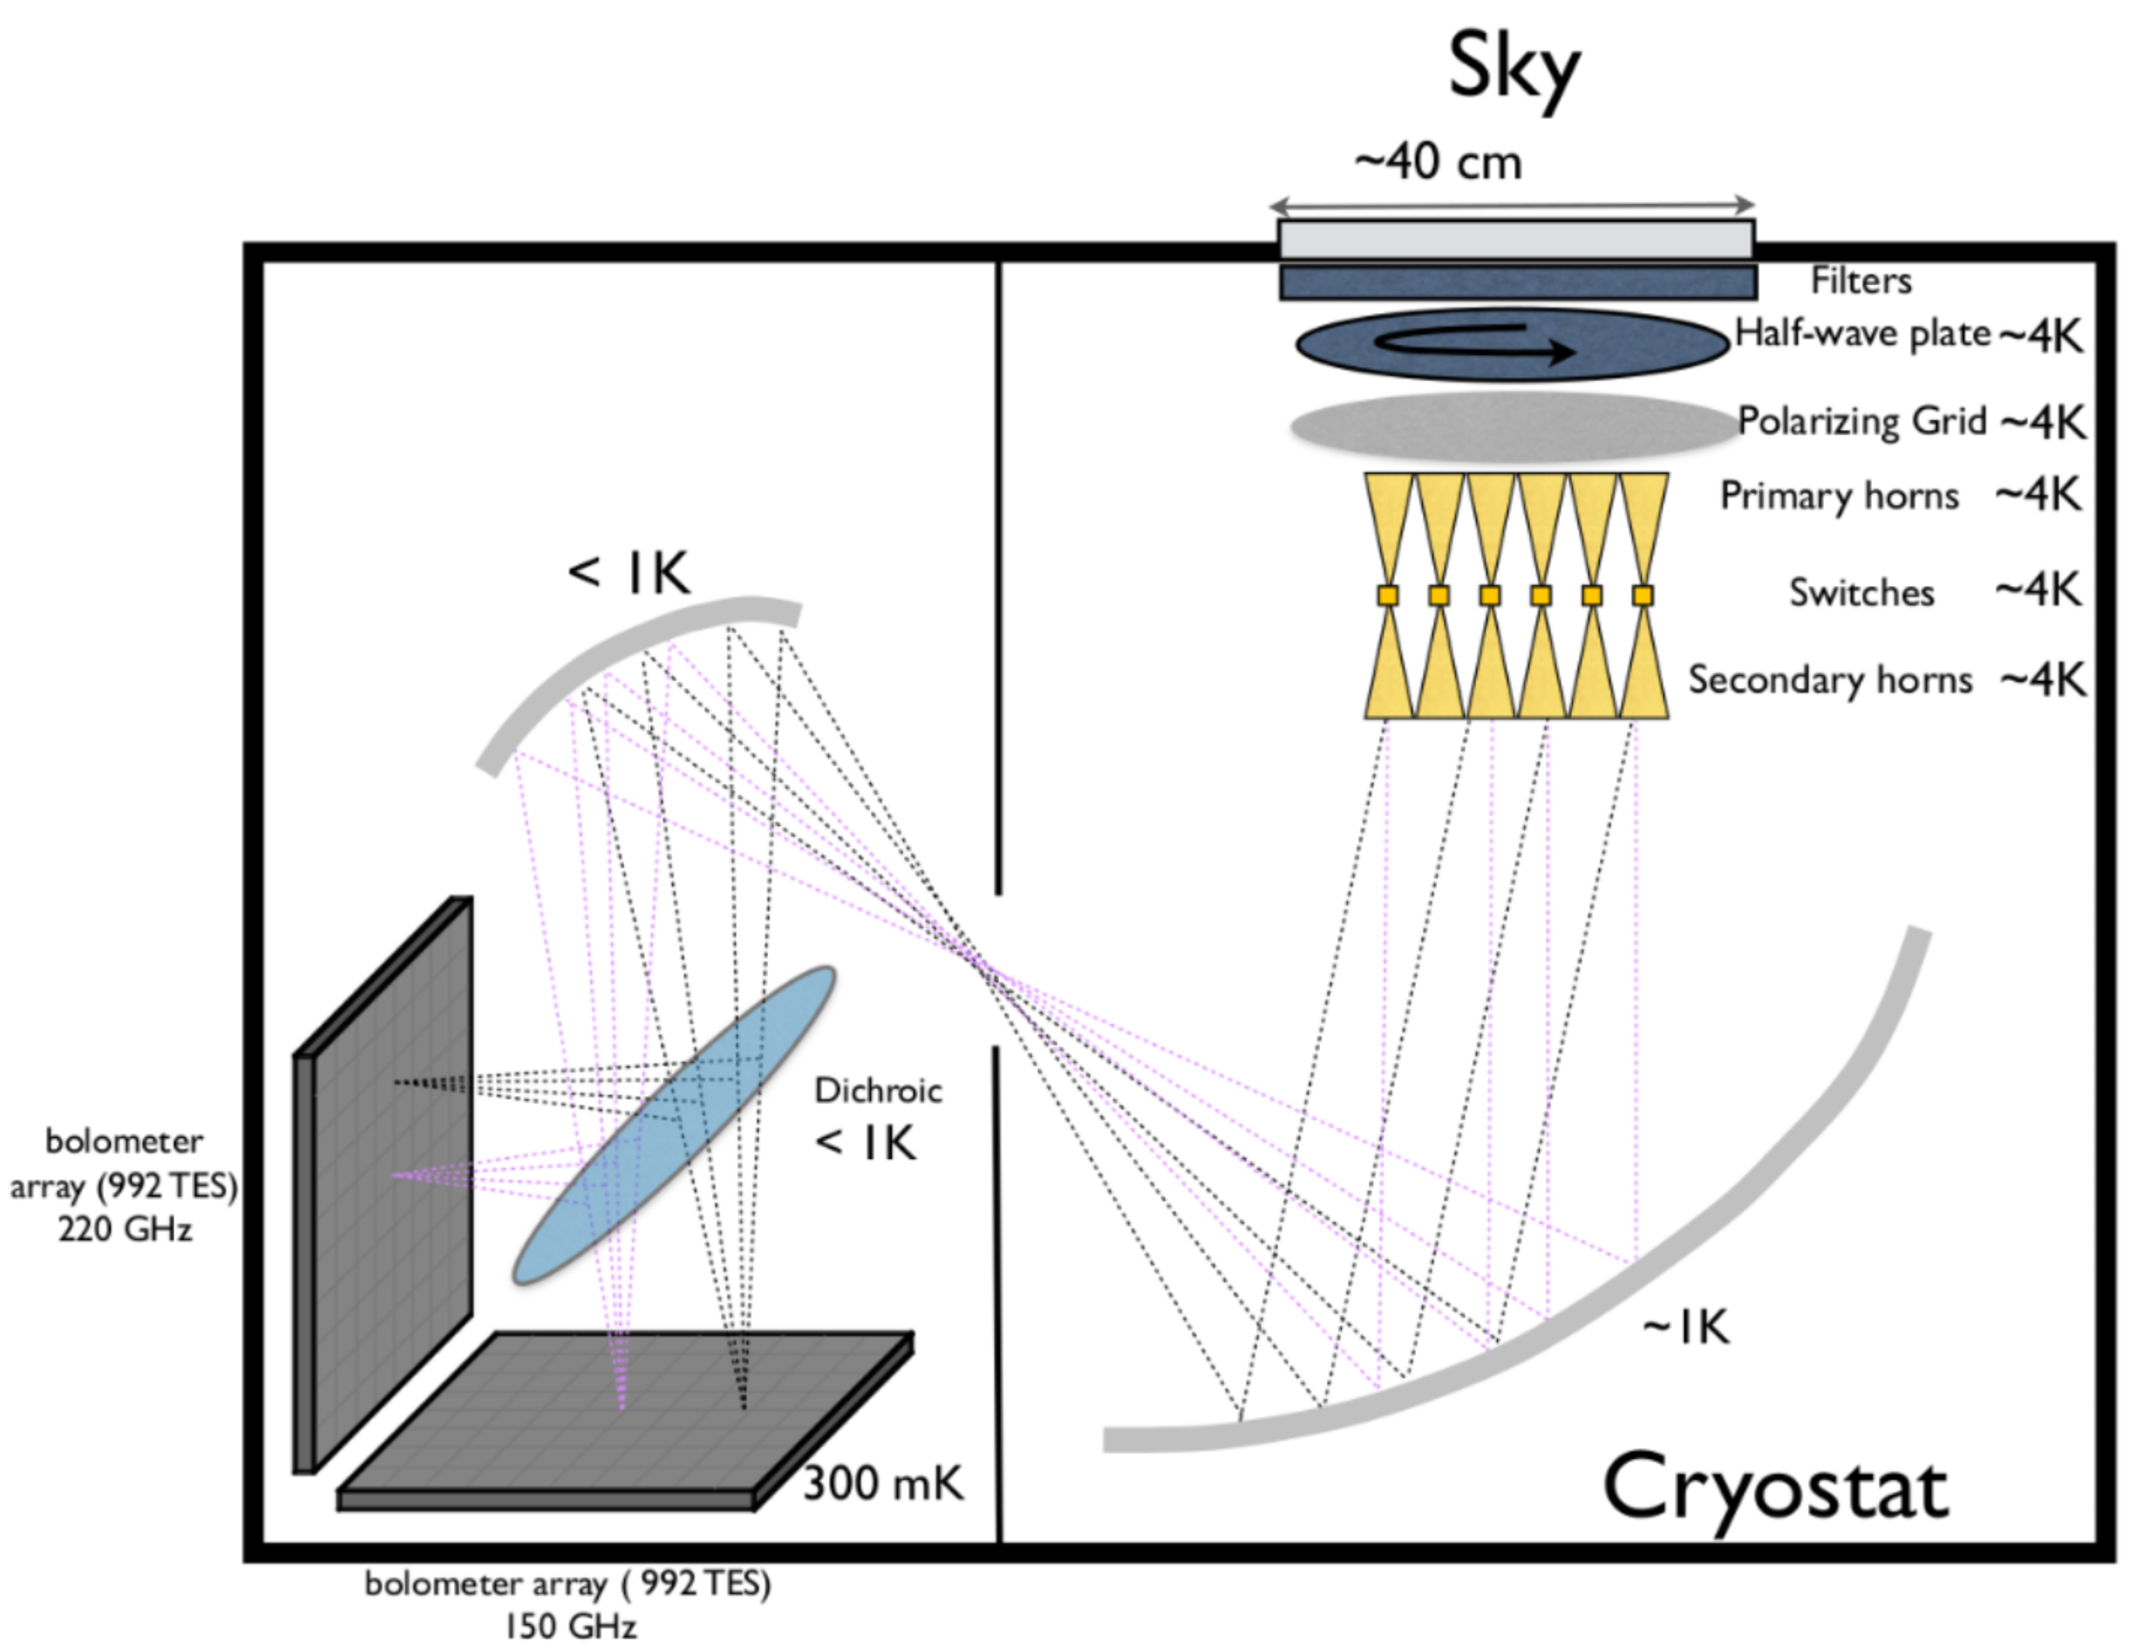
\includegraphics[width=0.6\textwidth]{qubic2}}
												\only<3>{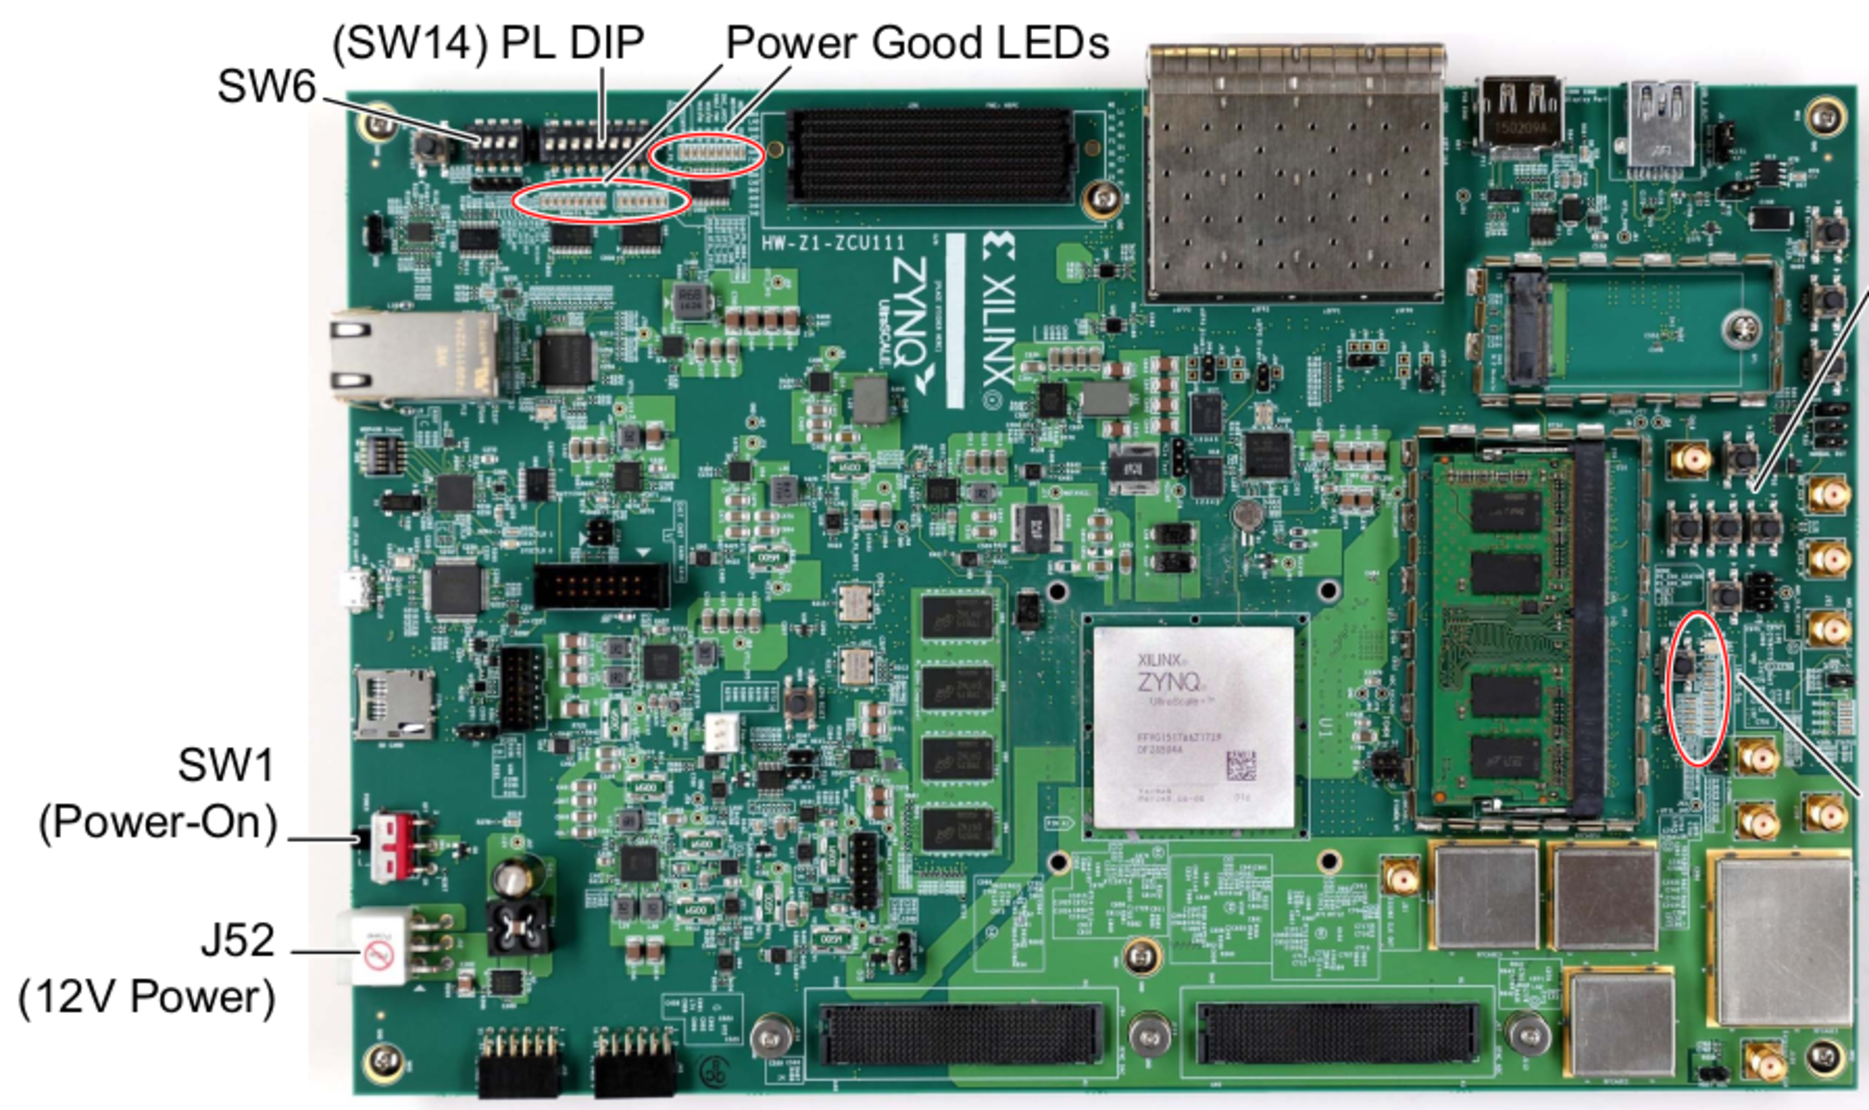
\includegraphics[width=0.7\textwidth]{zcu2}}

\end{frame}

%------------------------------------------------------------------------------
\section{MKIDs}
\begin{frame}{\textbf{M}icrowave \textbf{K}inetic \textbf{I}nductance
				\framesubtitle{Detectores superconductores}
				\textbf{D}etector (MKID)}
				\centering
												\qquad 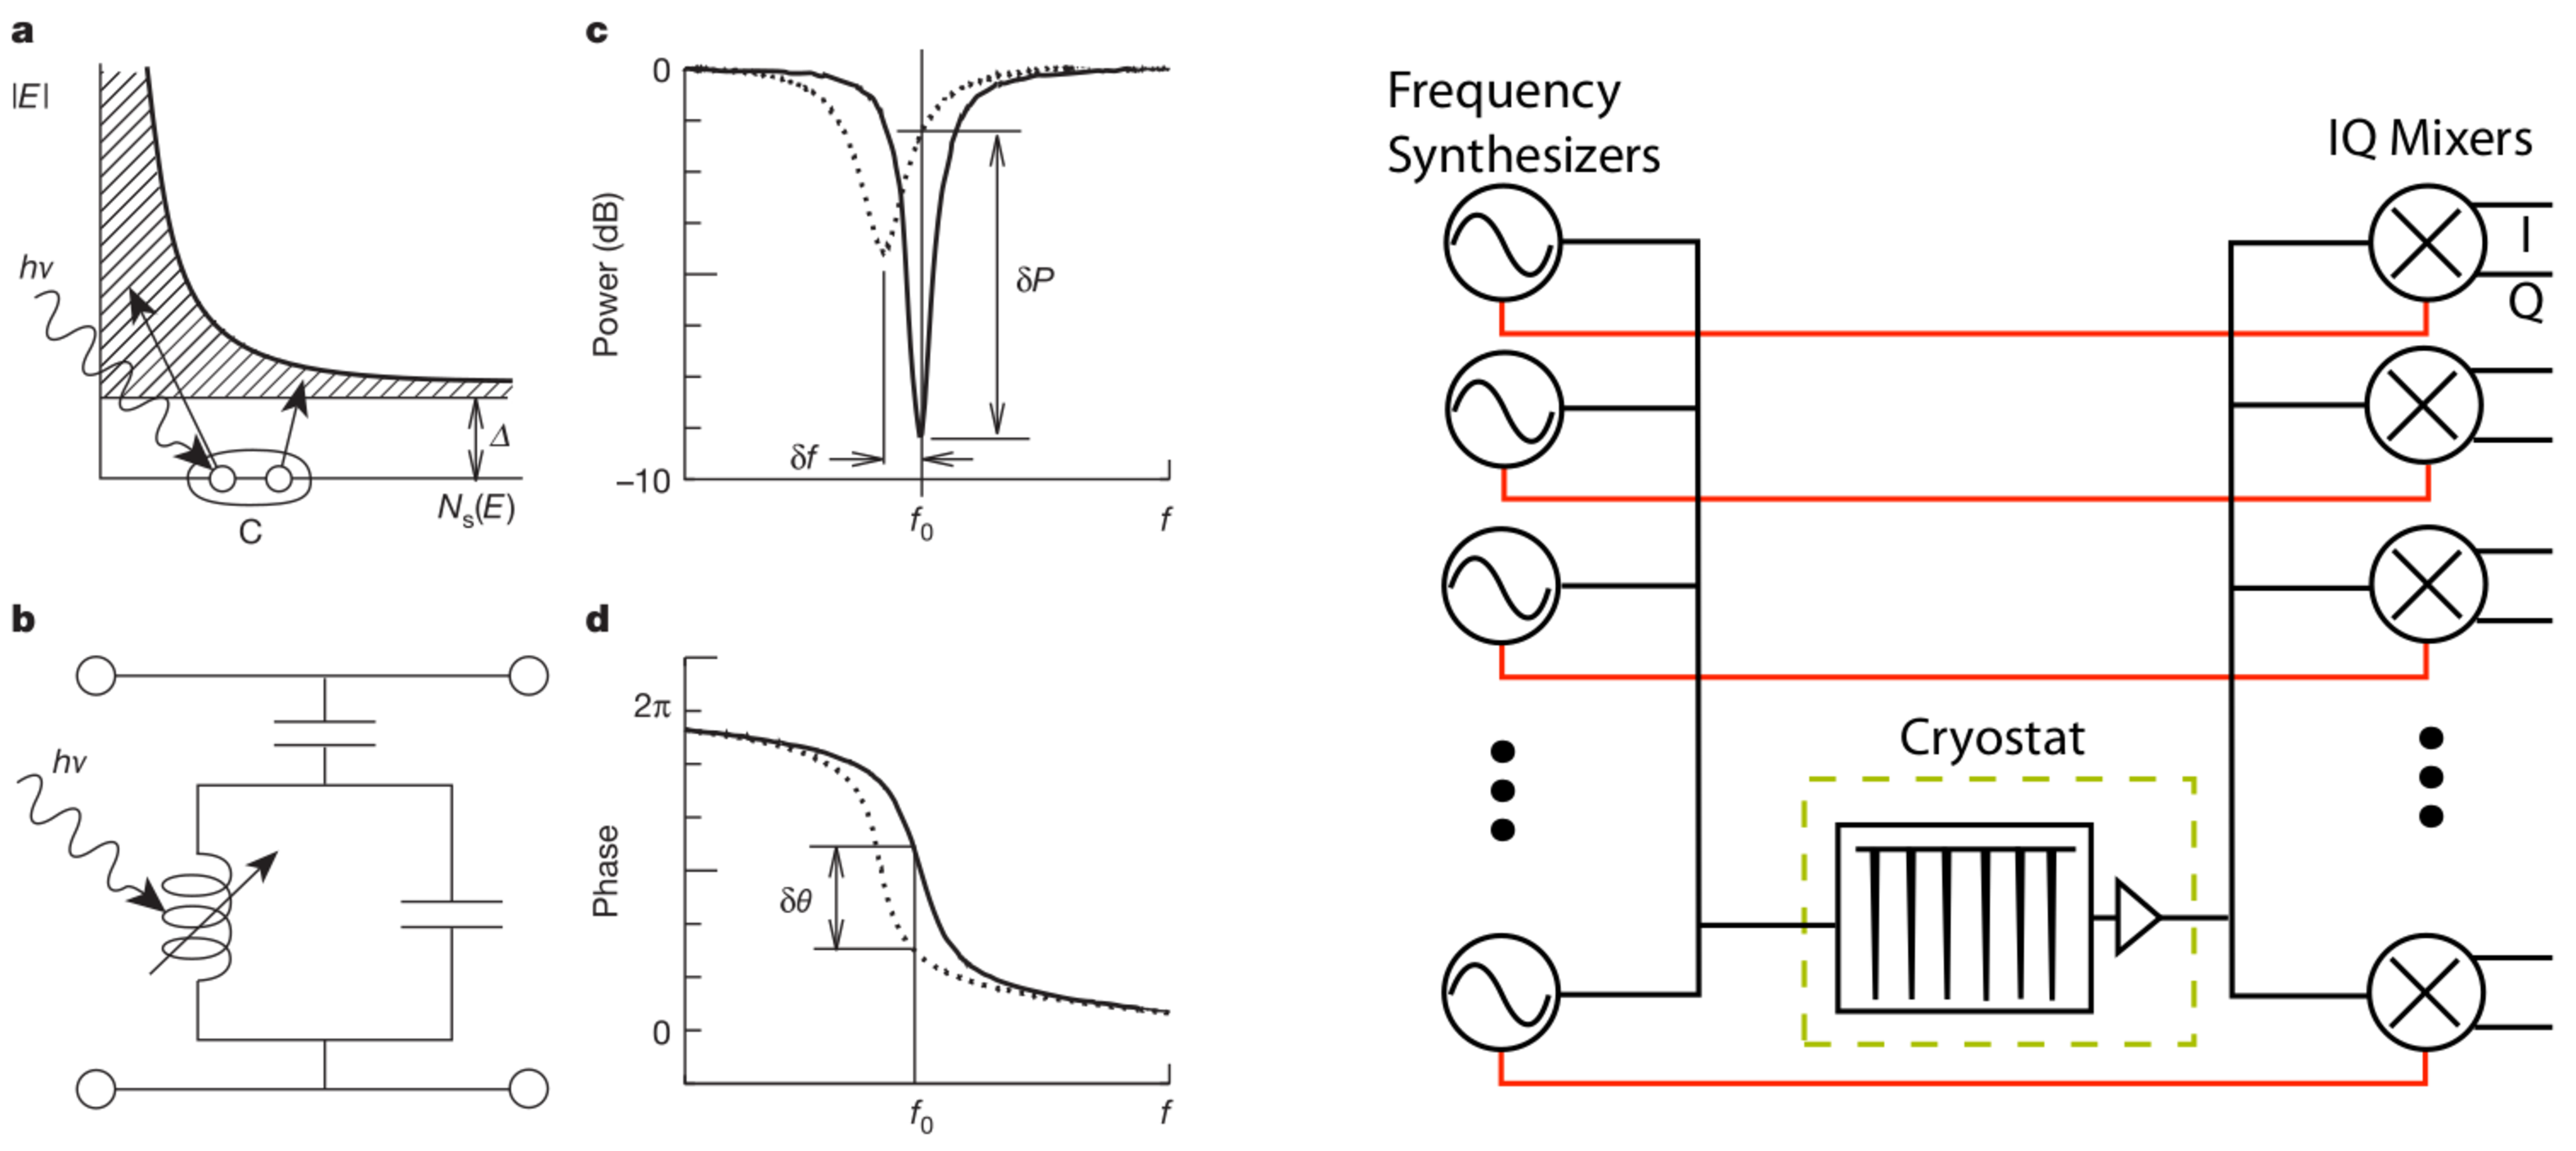
\includegraphics[width=0.8\textwidth]{concepto_mkid1}
				\begin{itemize}
								\item \footnotesize{Superconductores $\to$ inductancia AC debida a la
												inercia de los pares de Cooper}
								\item Cambia cuando los pares de Cooper se rompen debido a la
												energía de entrada
								\item Se mide el cambio monitoreando un circuito resonante

								\item Punto crítico $\to$ los \alert{superconductores proveen un muy
												alto Q} ($Q_i > 10^7$) $\to$ \tikzmark{start}miles de resonadores
												pueden ser leídos a través de una sola
												linea\tikzmark{end} 
												\begin{itemize}
																\item[*] \scriptsize{{\color{blue}componentes de lectura criogénica muy
																				simples}}
												\end{itemize}
				\end{itemize}
				\begin{tikzpicture}[remember picture,overlay]
								\draw<2>[red,ultra thick,rounded corners](-6.0,1.2) rectangle (4.4,1.8);																%\node<2>[draw,line width=2pt,cyan,circle,fit={(pic cs:start) (pic cs:end)}] {};
				\end{tikzpicture}
\end{frame}
\begin{frame}{\textbf{M}icrowave \textbf{K}inetic \textbf{I}nductance
				\textbf{D}etector (MKID)}
				\framesubtitle{Detectores superconductores}
				\begin{columns}
								\begin{column}{0.49\textwidth}
												\begin{equation*}
																Z_s = R_s + j \omega L_s
												\end{equation*}
												\begin{equation*}
																L_s = L_g + L_k
												\end{equation*}

												\flushleft	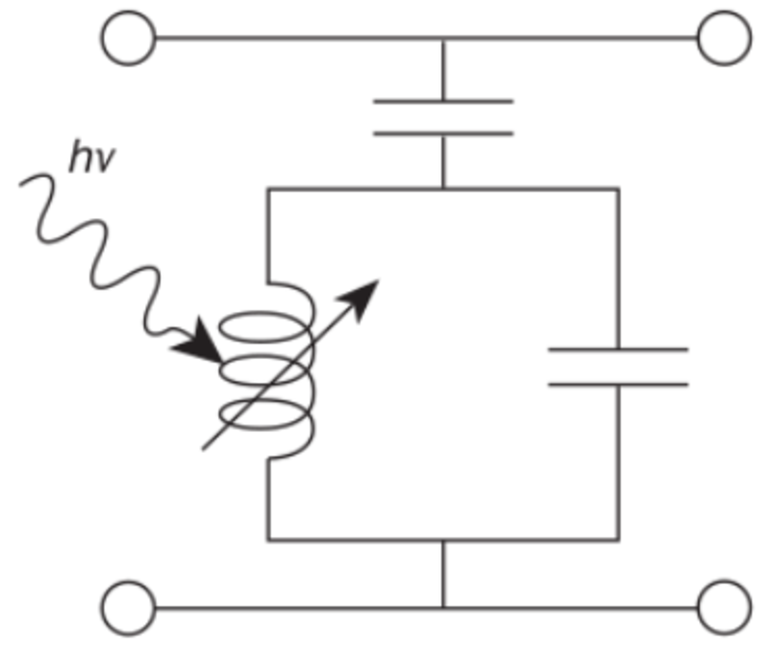
\includegraphics[width=0.8\textwidth]{LCR_mkid}
								\end{column}
								\begin{column}{0.59\textwidth}
												\begin{itemize}
																\item[o] $R_s \to$ pérdidas A.C. debidas a $e^-$ no apareados
																				(pares de Cooper)
																\item[o] $L_s \to$ inductancia superficial total
																\item[o] $L_g \to$ inductancia geométrica
																\item[o] $L_k \to$ inductancia cinética
																				({\color{blue}dependiente de T}), además
												\end{itemize}

												\begin{equation*}
																L_k \propto 1/T_c
												\end{equation*}

												\begin{equation*}
																f_r = \frac{1}{\sqrt{C_g(L_g + L_k)}}
												\end{equation*}
								\end{column}
				\end{columns}
\end{frame}

%------------------------------------------------------------------------------
\section{Desarrollo del sistema de lectura}
\begin{frame}{Desarrollo del sistema de excitación/lectura}
				\framesubtitle{Temas a considerar}
				\begin{columns}
								\begin{column}{0.5\textwidth}
												\footnotesize{\begin{itemize}
																\item Algoritmo de procesamiento de señales
																\item Selección de frecuencia, velocidad de datos de salida
																\item Ruido, potencia, rango dinámico
																\item $f$ espúreas, productos de intermodulación, etc.
																\item Implementación: ubicación, empaque, fuente de
																				energía, comunicación, interfaz con PC, etc.
												\end{itemize}}
												\begin{center}
																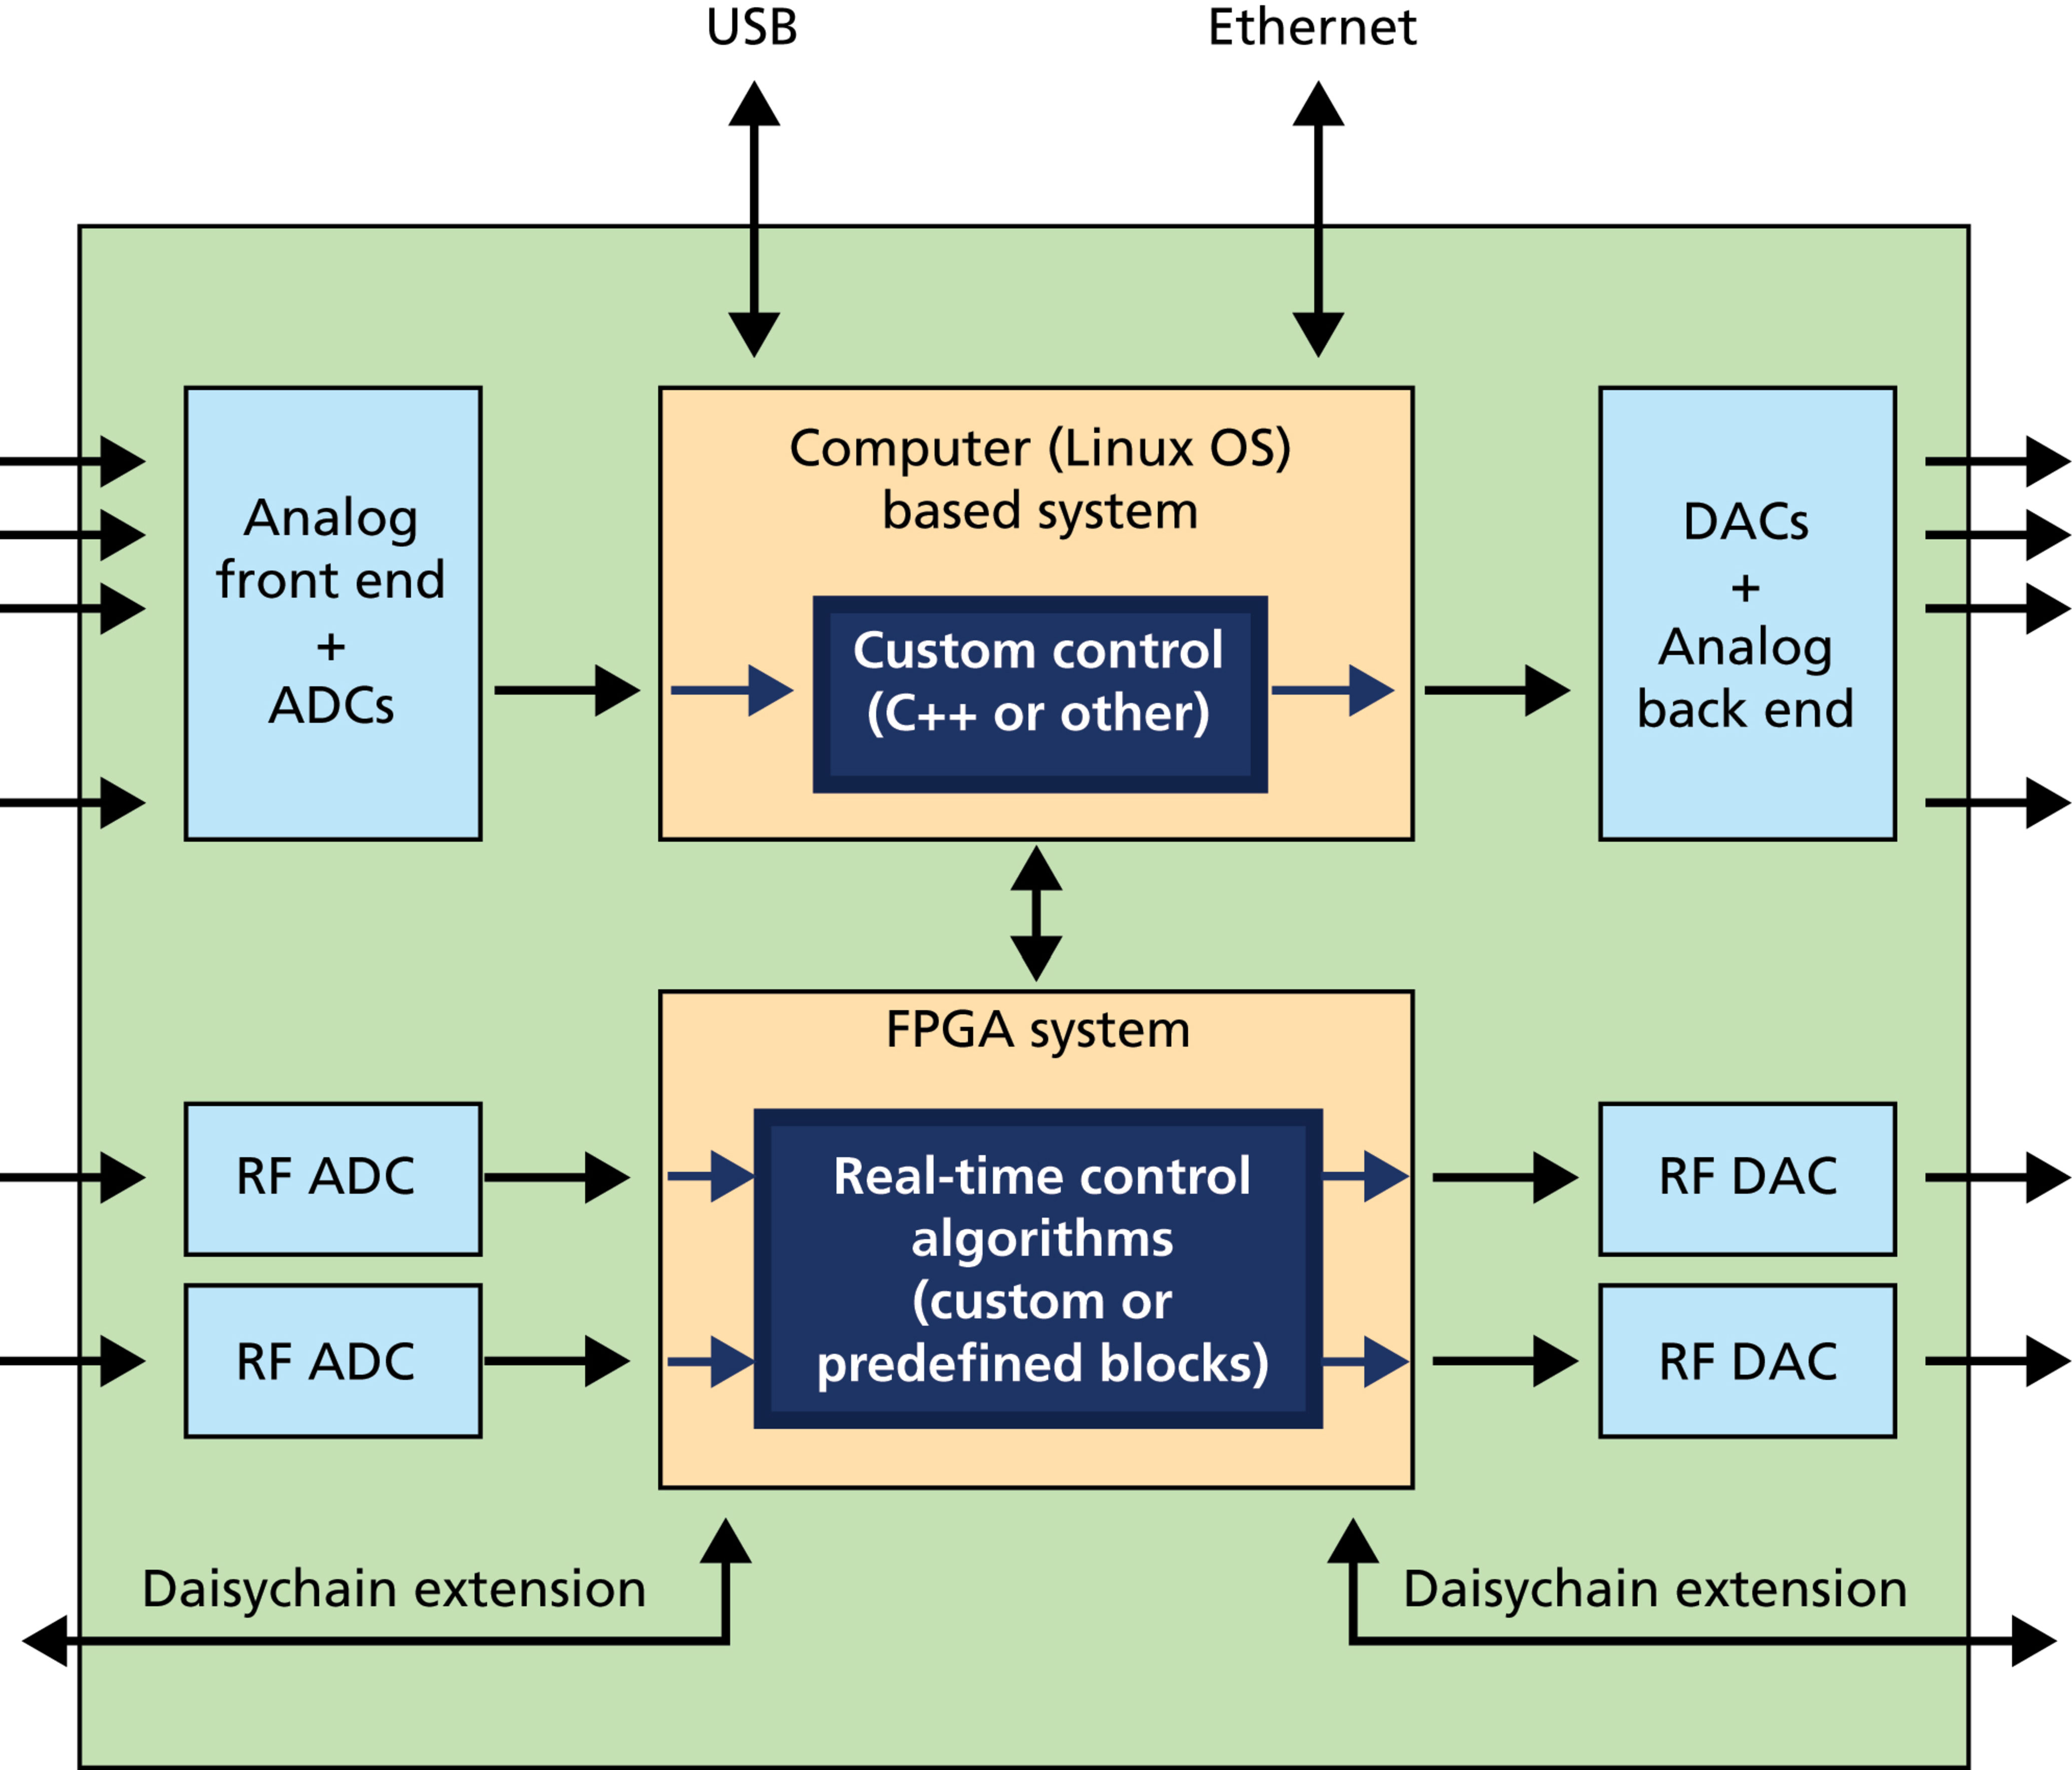
\includegraphics[width=0.6\textwidth]{rp_como_sistema}
												\end{center}
								\end{column}
								\begin{column}{0.5\textwidth}
												STEMLab RedPitaya
												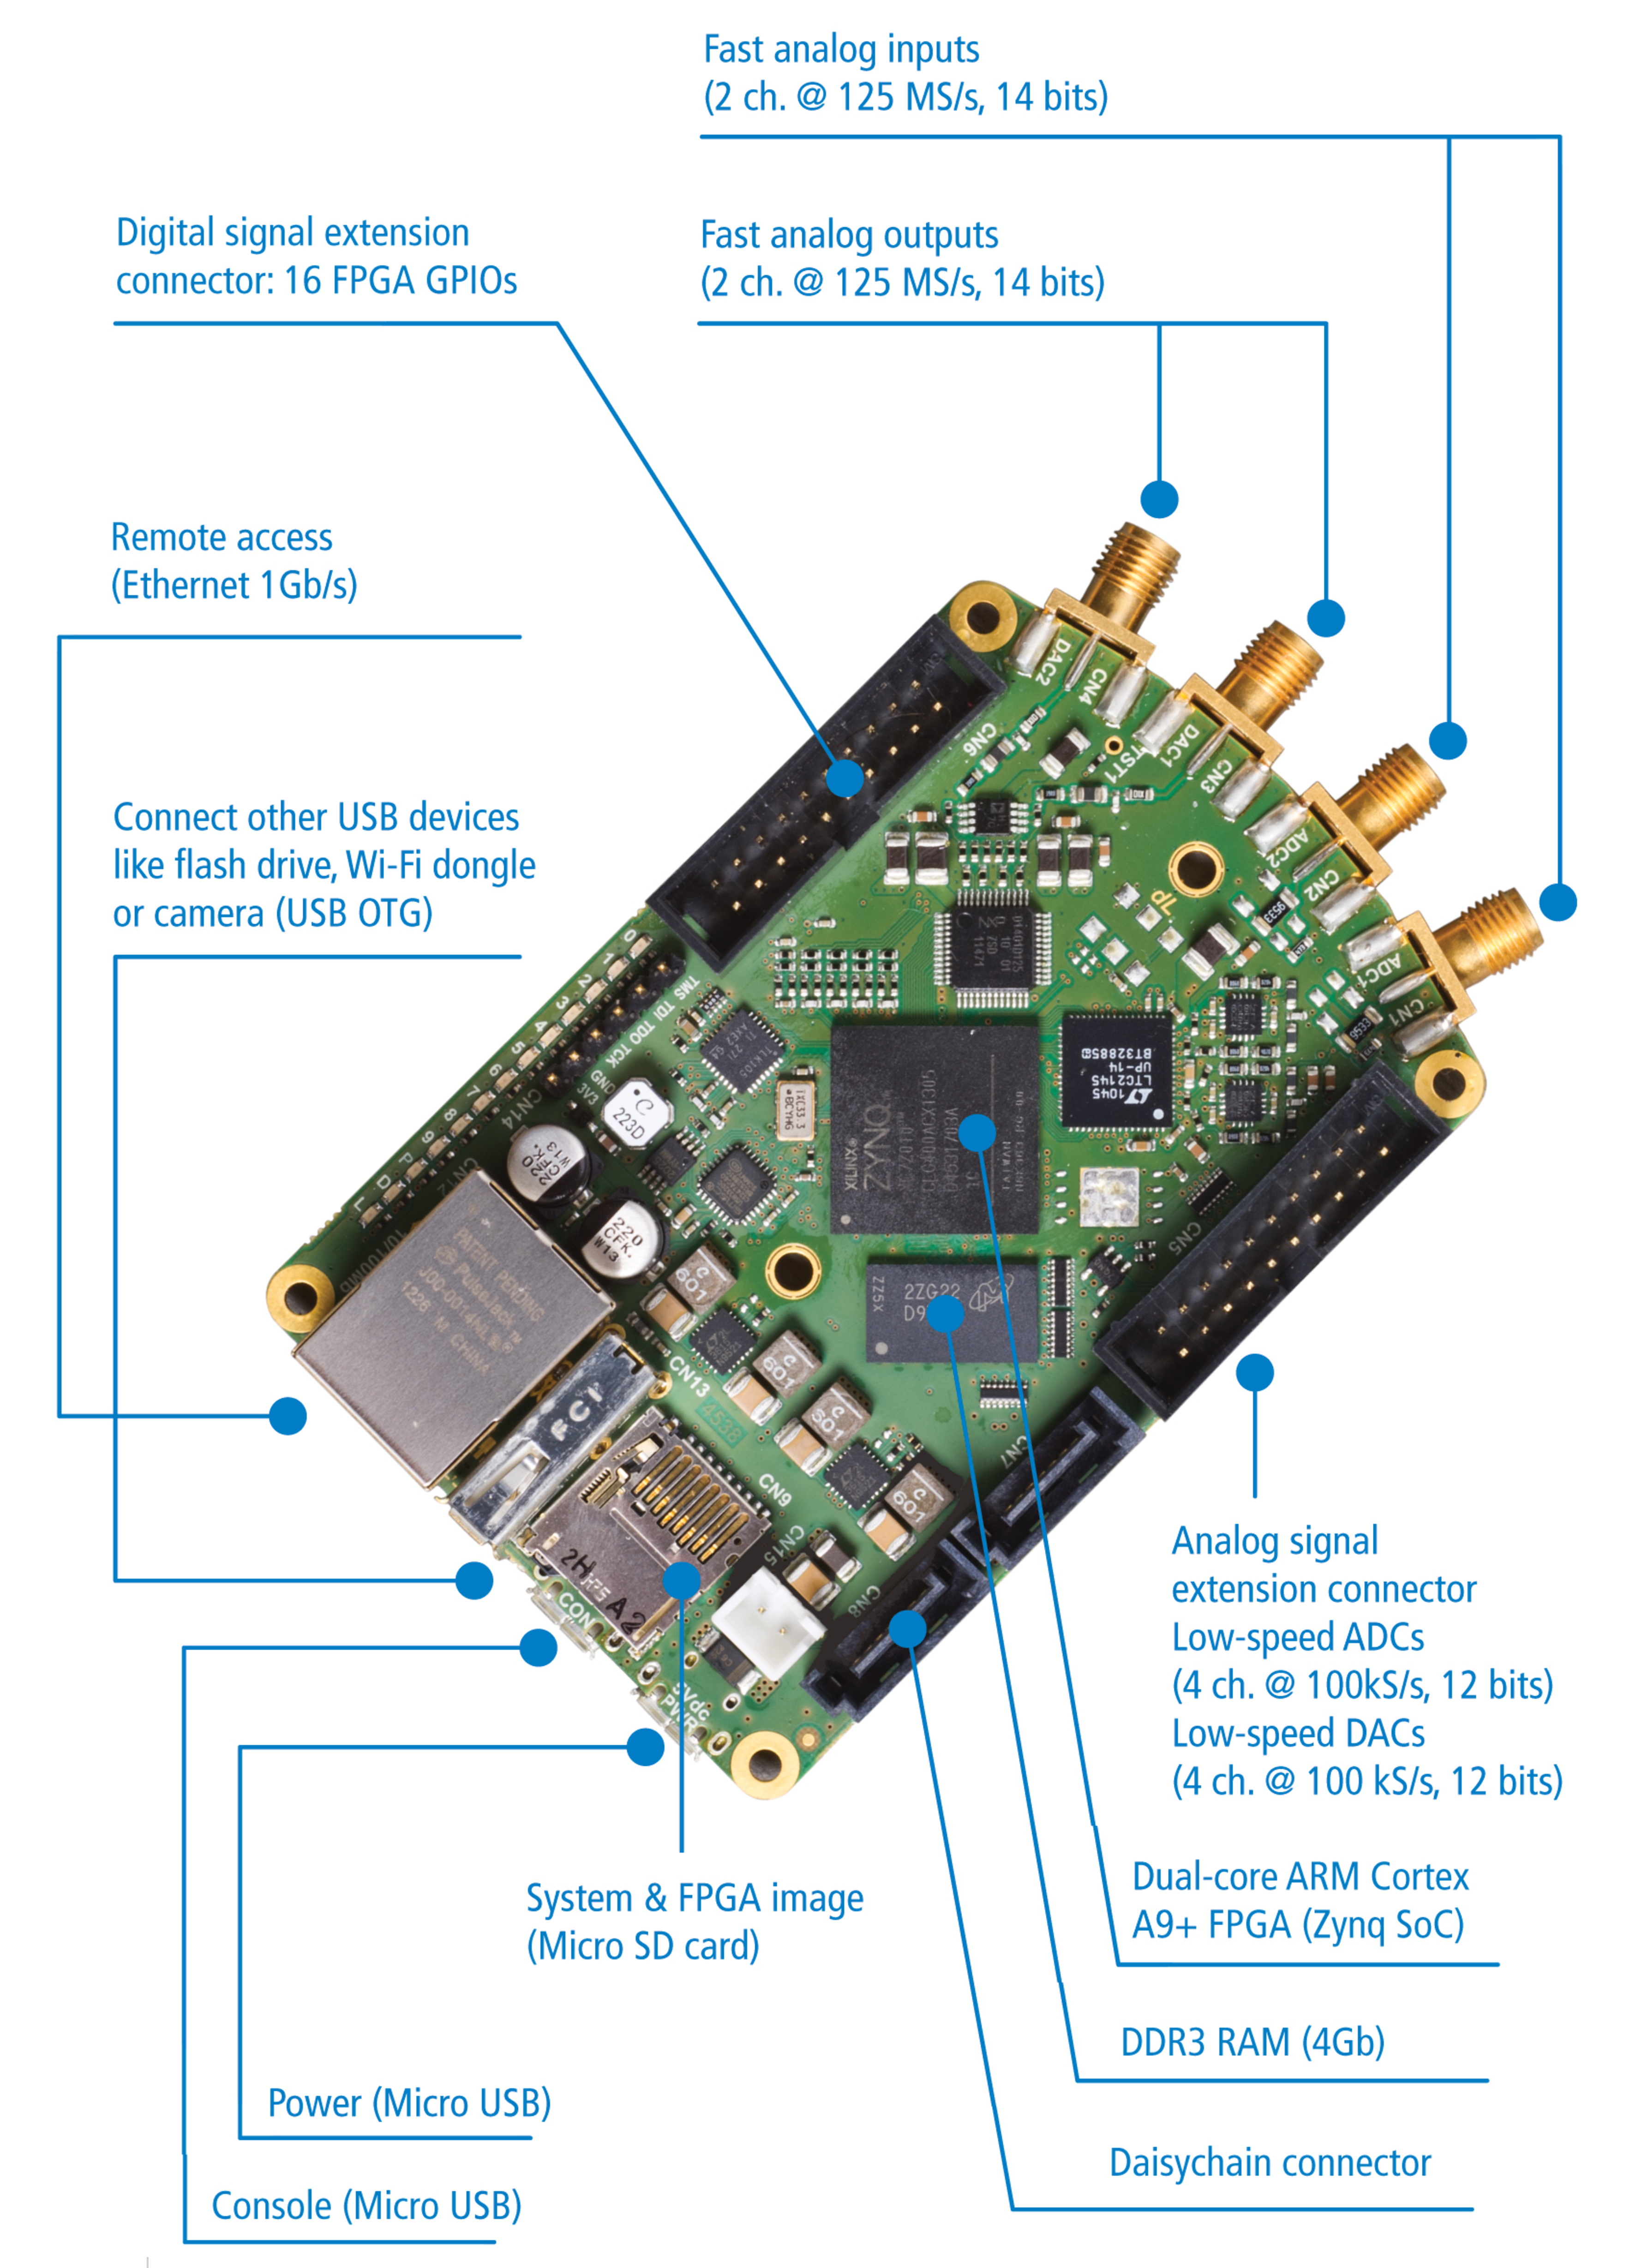
\includegraphics[width=0.8\textwidth]{rp_sistema_2}
												%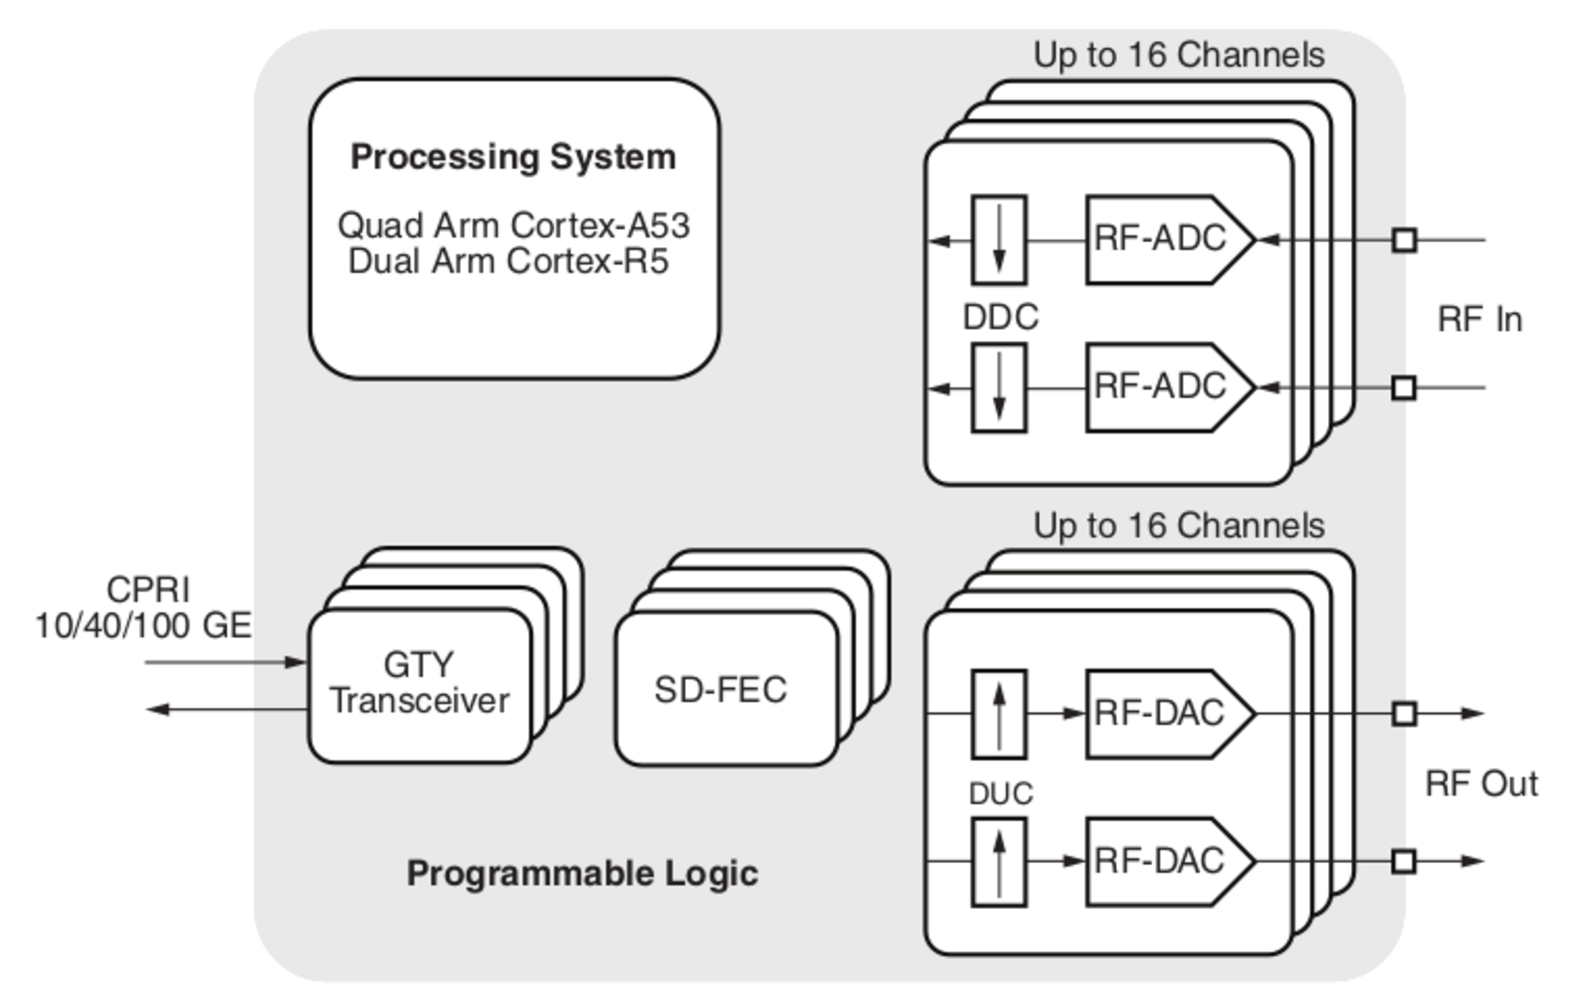
\includegraphics[width=0.8\textwidth]{zcu1}
												%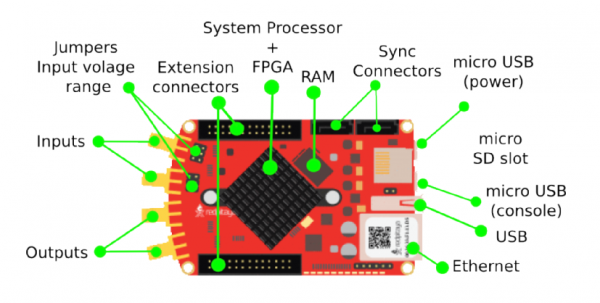
\includegraphics[width=0.8\textwidth]{600px-RedPitaya_HW_overview}
								\end{column}
				\end{columns}
\end{frame}

\begin{frame}{Desarrollo del sistema de excitación/lectura}
				\framesubtitle{Temas a considerar}
				\centering
				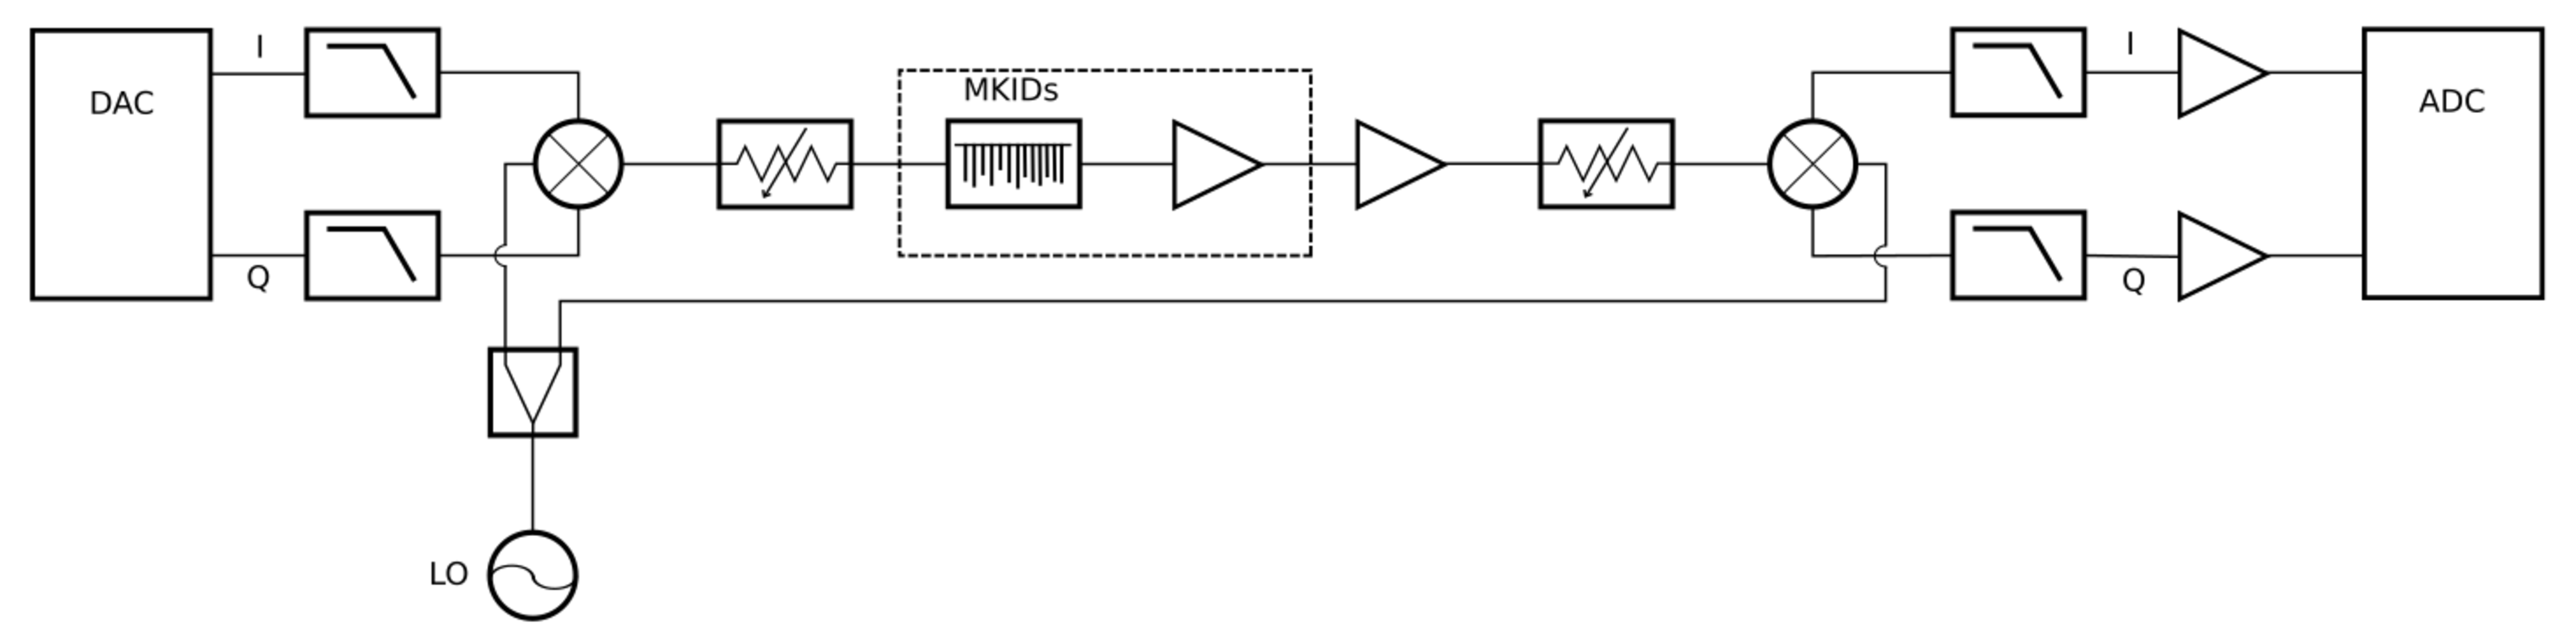
\includegraphics[width=\textwidth]{readout1}

				\begin{itemize}
								\item Ruido \alert{dominado por el amplificador criogénico},
												$T_\text{ruido} \sim$ 2 a 5\,K 
								\item \alert{El chip ADC será el próximo factor
												limitante para el ruido de lectura}
								\item	$f_s$ se elige para que
												coincida con el ancho de banda del resonador
								\item $p_\text{max} \propto	n^{1/2}\,\text{para}\,n >> 1$
				\end{itemize}

				%\tiny{\emph{\textbf{An open-source readout for MKIDs}}, Proc. SPIE Astron.
				%Telesc.  Instrum., doi:10.1117/12.856832}
\end{frame}

\begin{frame}{Desarrollo del sistema de excitación/lectura}
				\framesubtitle{Frequency Division Multiplexing (FDM)}
				\begin{columns}
								\begin{column}{0.5\textwidth}
												\begin{itemize}
																\item[o]	Estrategia de multiplexación poderosa\\
																				--\footnotesize{{\color{blue}Muchos detectores 
																				acoplados a una sola linea}}
																\normalsize{\item[o] Muchos canales por amplificador de microondas
																\item[o] Hardware criogénico: solo un amplificador y algunos
																				cables coaxiales}
												\end{itemize}
												\begin{center}
																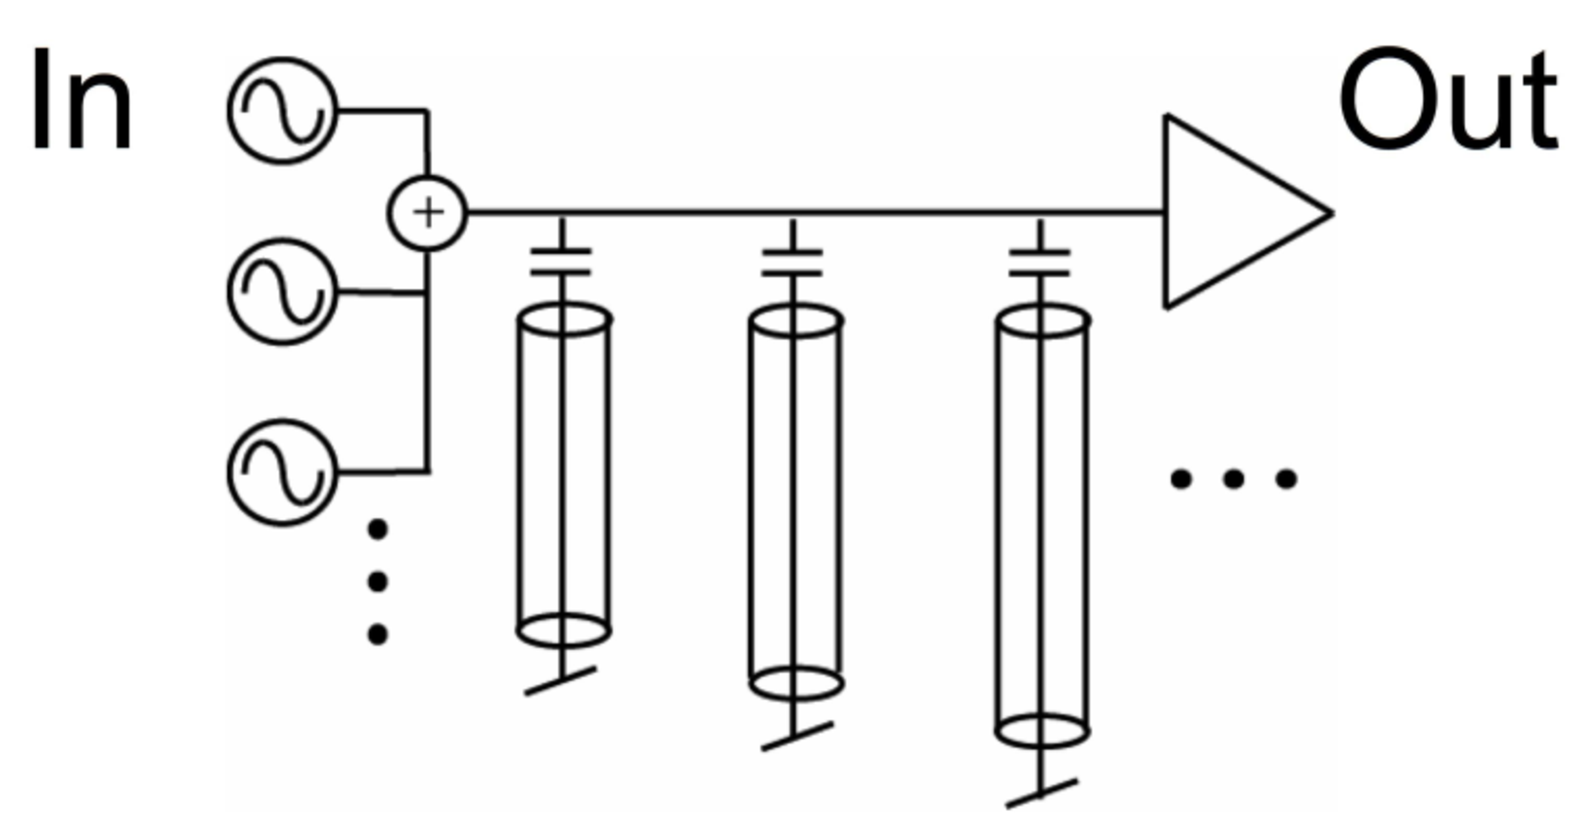
\includegraphics[width=\textwidth]{fdm1}
												\end{center}
								\end{column}
								\begin{column}{0.5\textwidth}
												\begin{center}
																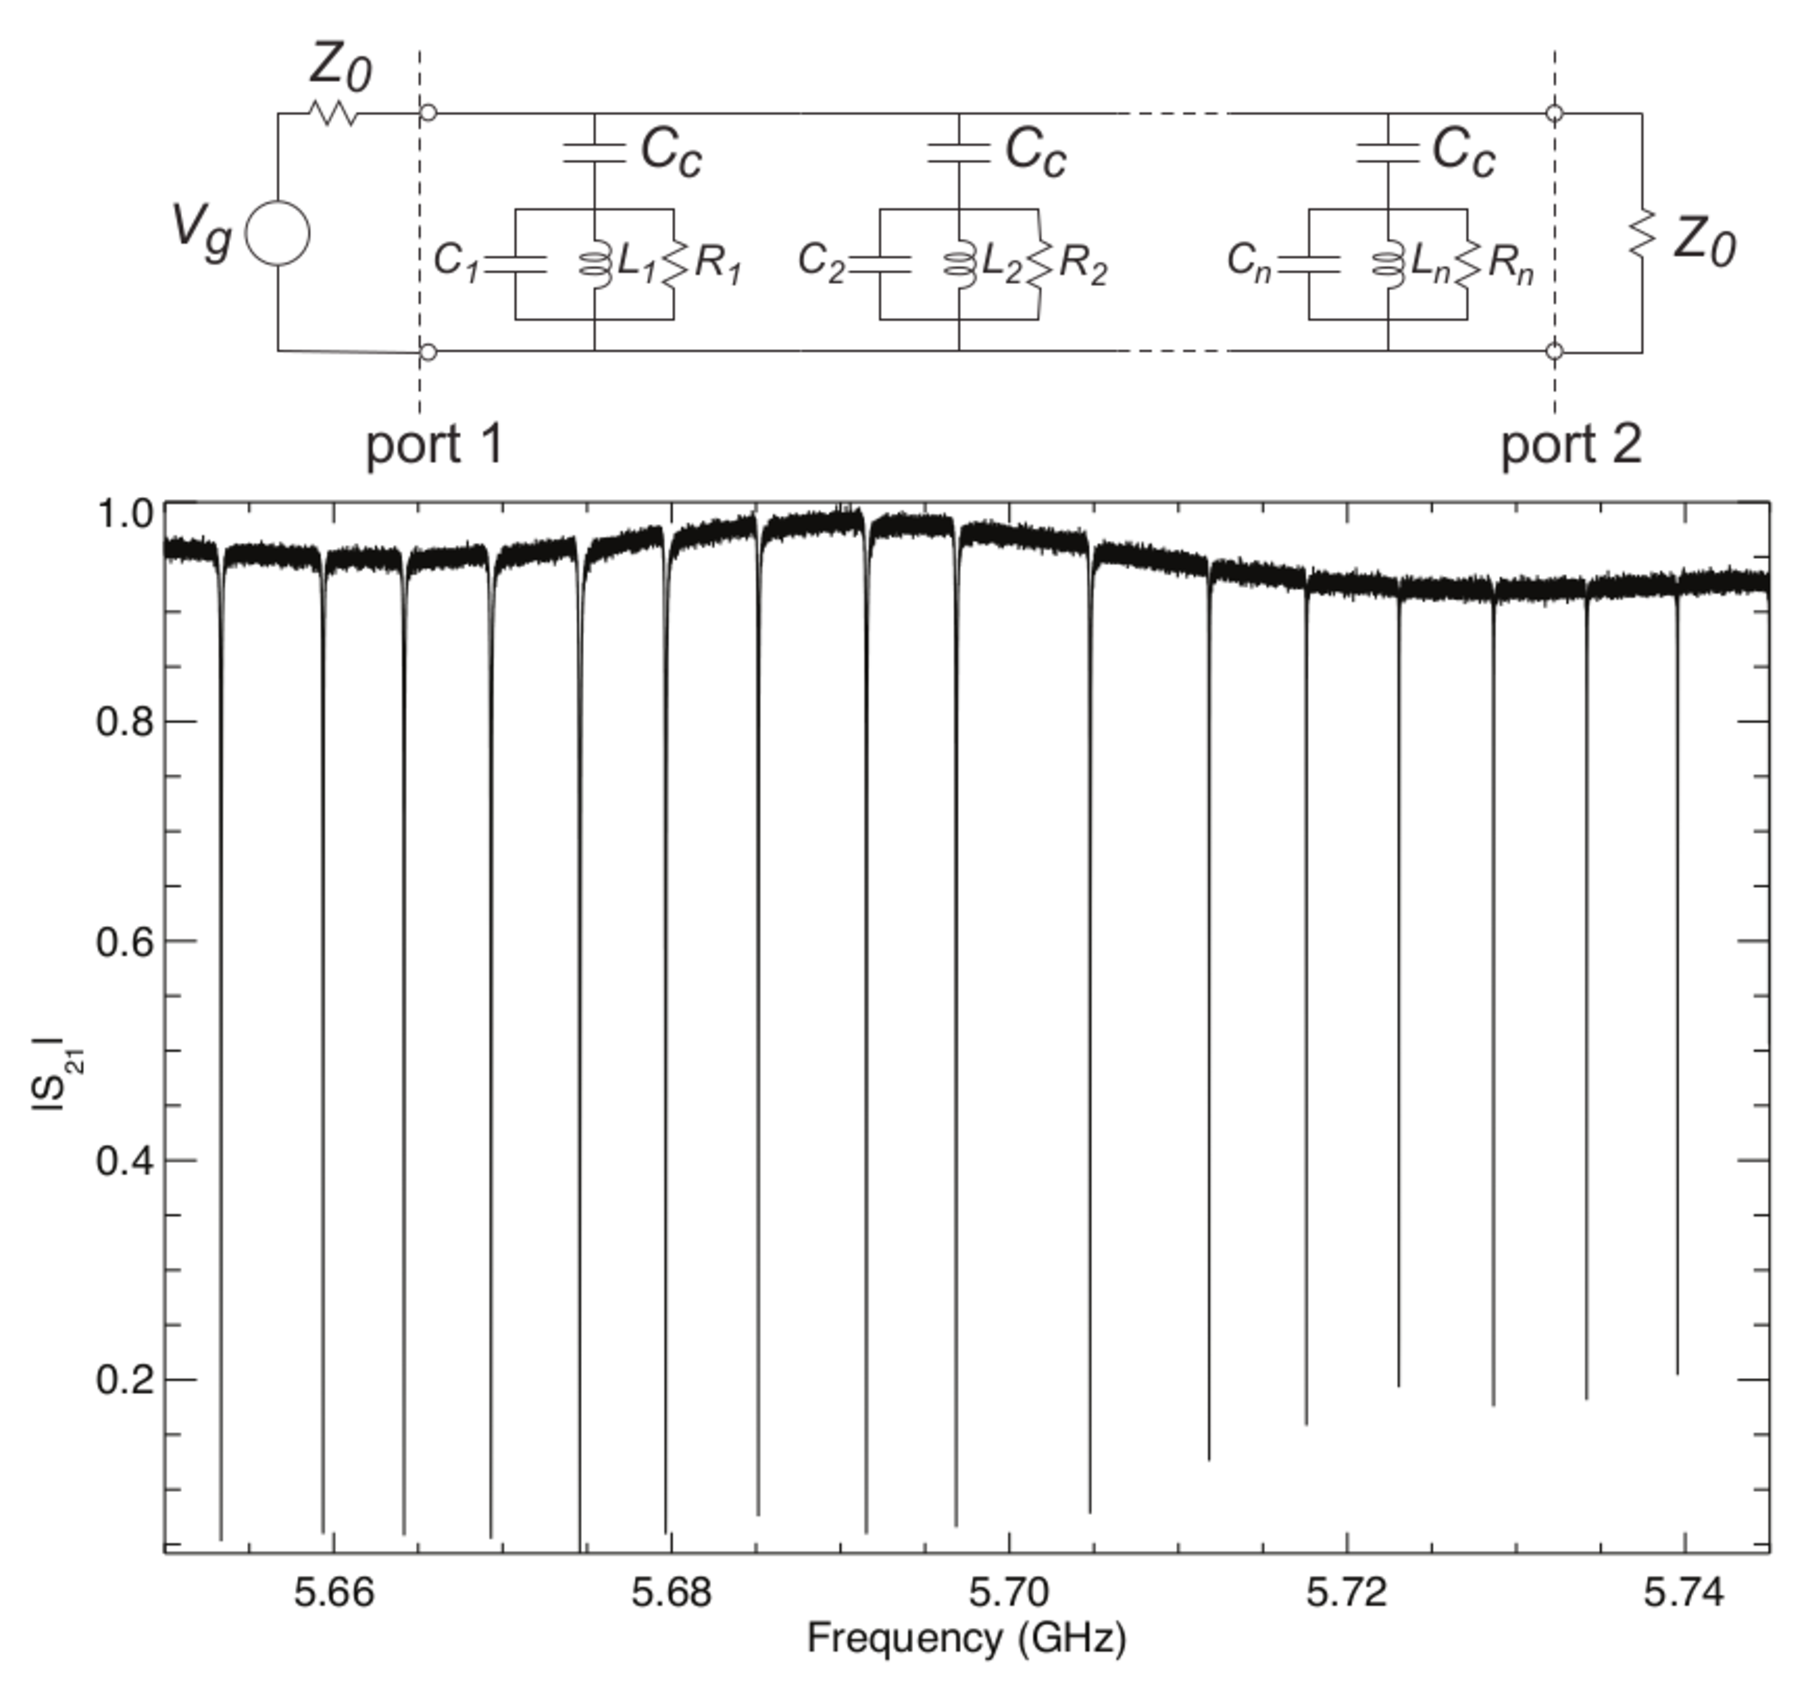
\includegraphics[width=\textwidth]{fdm2}
												\end{center}
								\end{column}
				\end{columns}

\end{frame}

\begin{frame}{Desarrollo del sistema de excitación/lectura}
				\framesubtitle{Canalizador DFT (Channelizer)}
				\begin{columns}
								\begin{column}{0.4\textwidth}
												\begin{itemize}
																\item[*] Implementación m\'as eficiente en t\'erminos de uso de hardware en FPGA
																\item[*] Ancho de banda similar para todos los
																				canales (DFT-PFB)
																\item[*] Extensible a un n\'umero grande de canales ($>=1000$)
																\item[*] Posibilidad de realizar el diseño en multi-etapas
												\end{itemize}
								\end{column}
								\begin{column}{0.6\textwidth}

												\begin{center}
																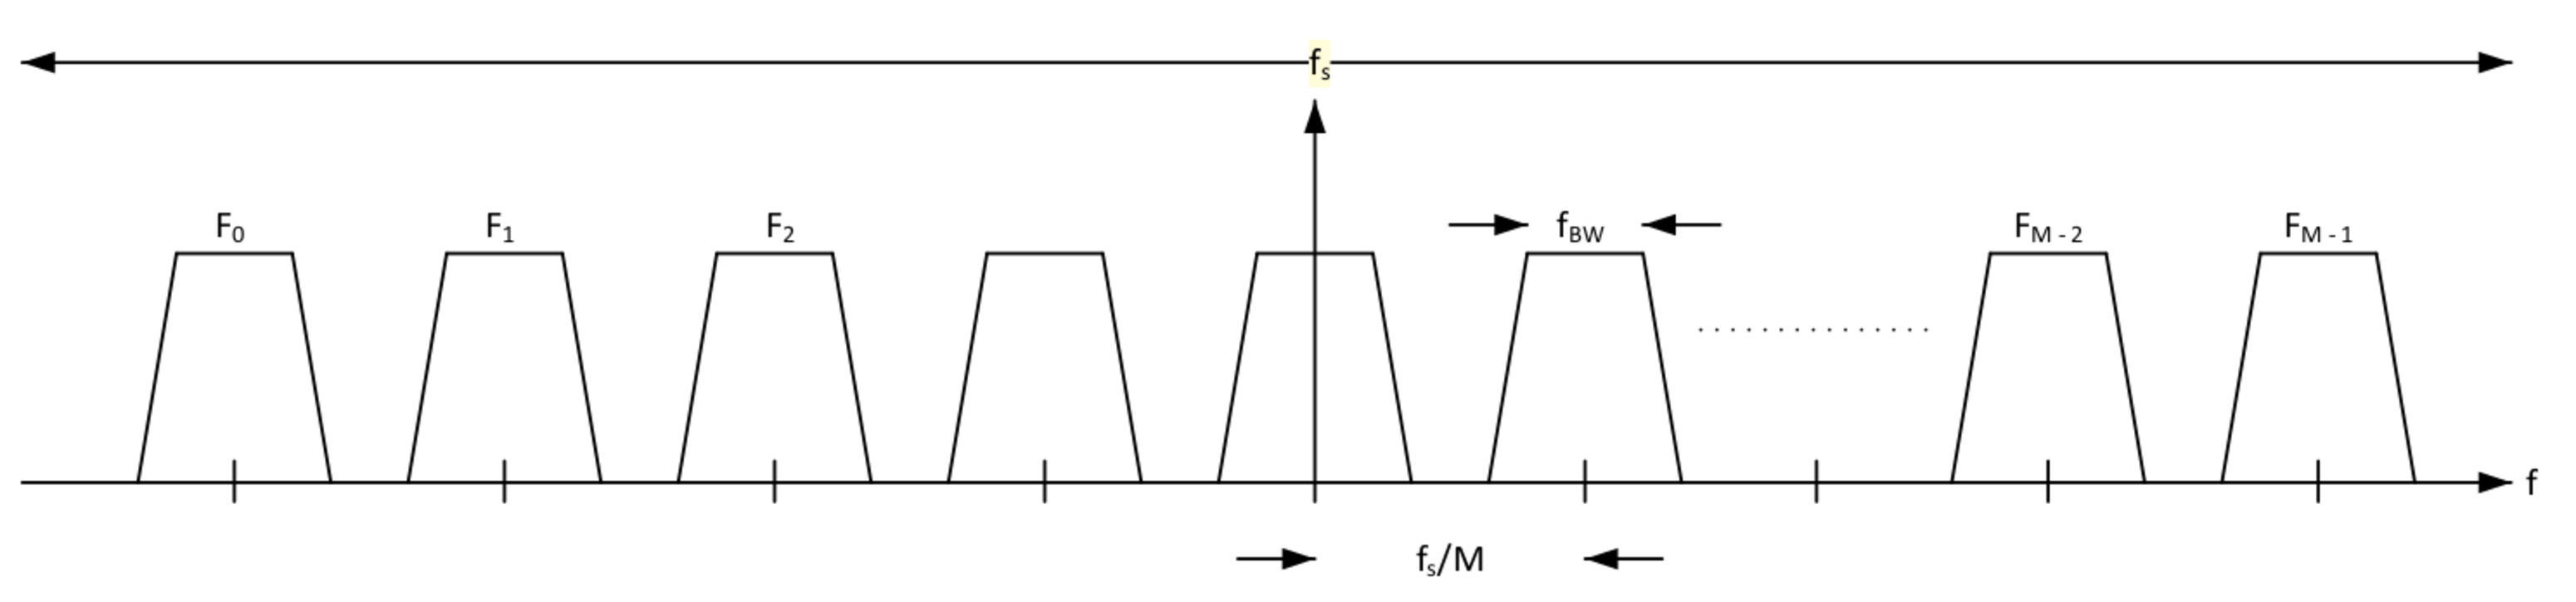
\includegraphics[width=\textwidth]{FDM_channel_diagram}
																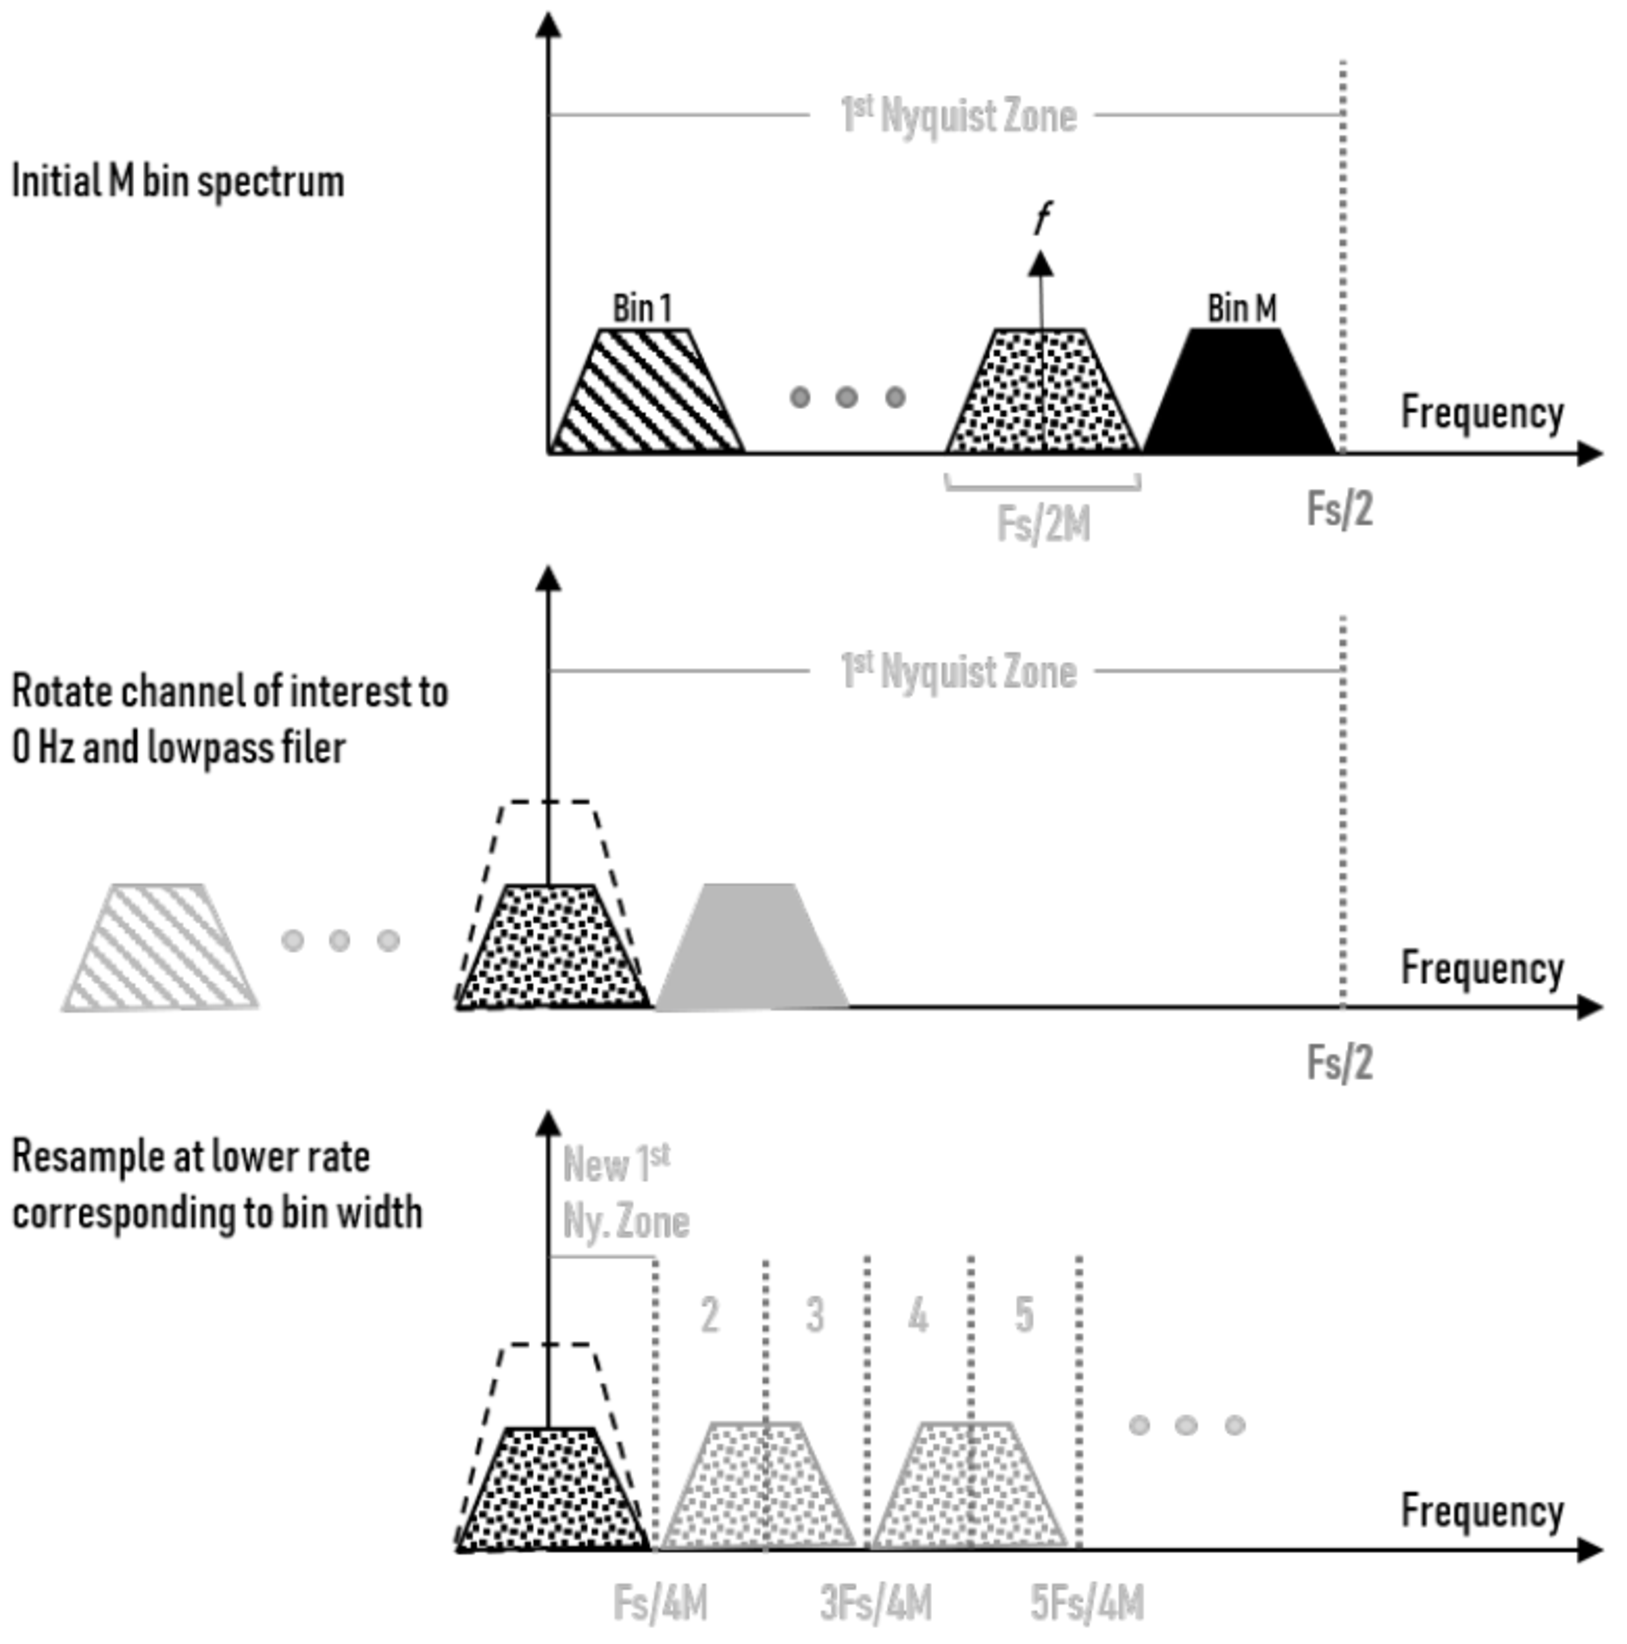
\includegraphics[width=0.9\textwidth]{pfb_basic1}
												\end{center}
								\end{column}
				\end{columns}
\end{frame}

\section{Channelizer}
\begin{frame}{Canalizador (Channelizer Tx/Rx)}
				\framesubtitle{D $\to$ downsampling ratio, M $\to$ número de canales, I
				$\to$ oversampling factor}
				\begin{itemize}
								\item D = M
								\item D $\neq$ M
								\item I = 2 
				\end{itemize}
				\begin{columns}
								\begin{column}{0.5\textwidth}
												\only<1>{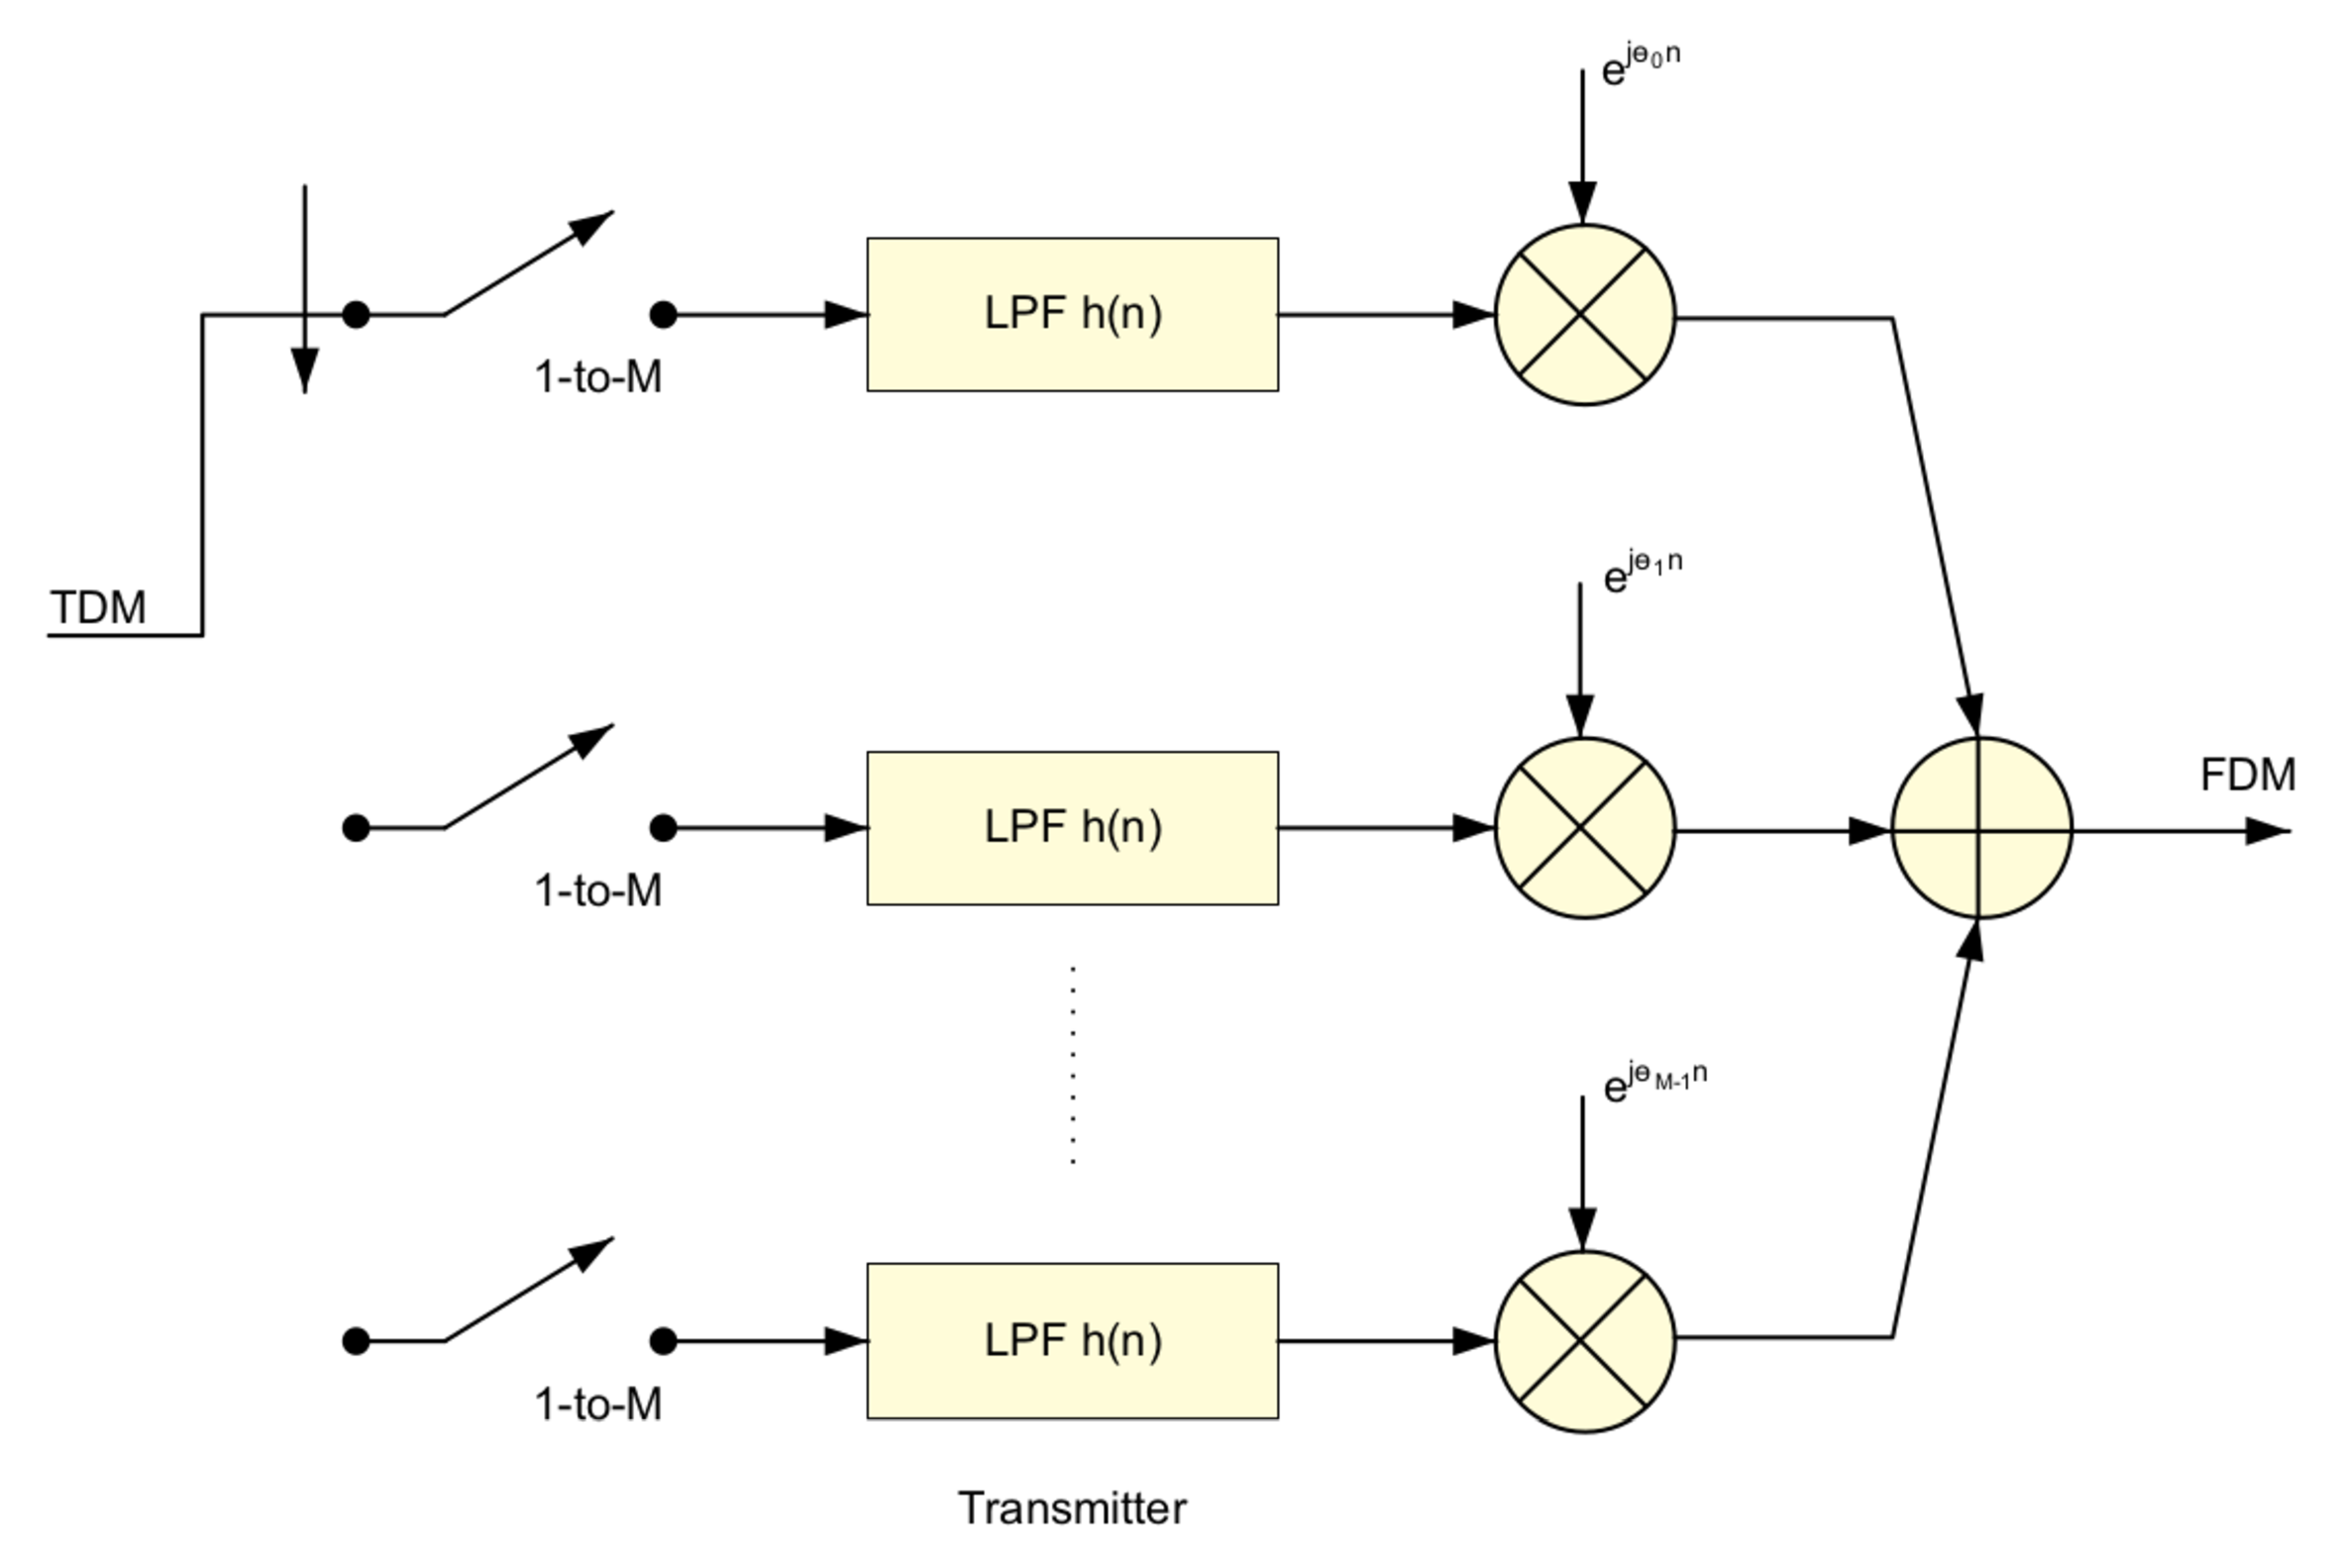
\includegraphics[width=1.09\textwidth]{Tx_channelizer}}
												\only<2>{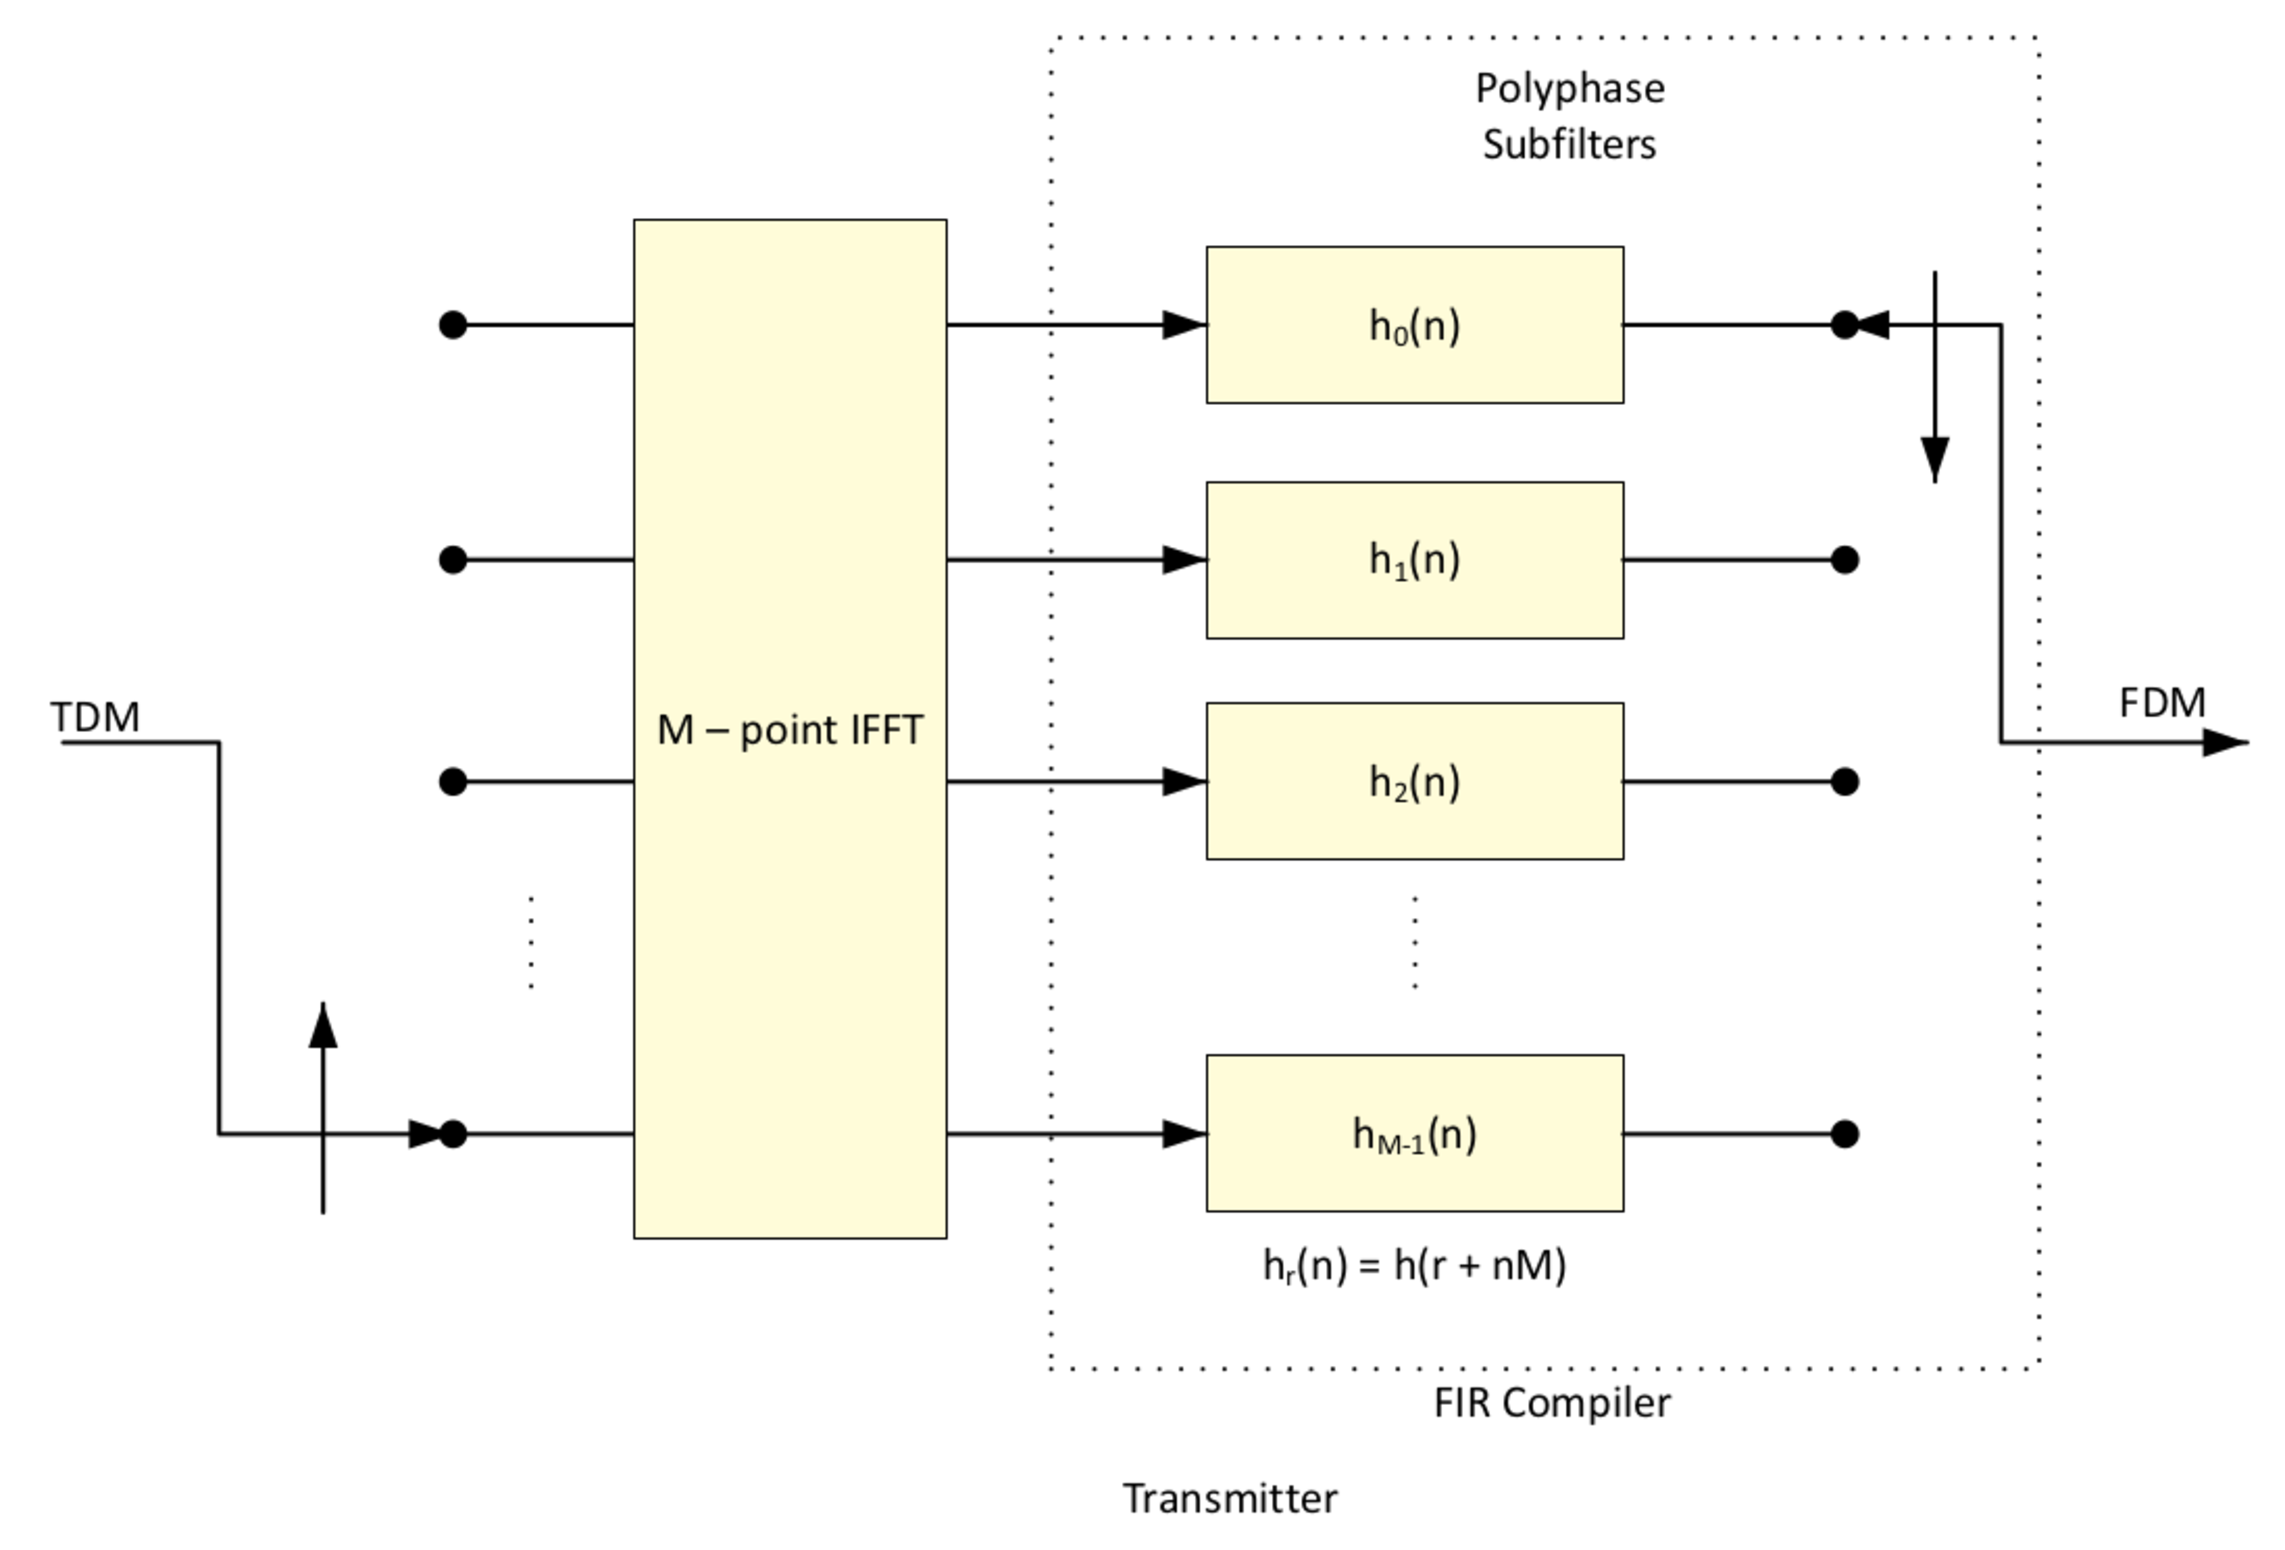
\includegraphics[width=1.09\textwidth]{Tx_channelizer_con_IFFT}}
								\end{column}
								\begin{column}{0.5\textwidth}
												\only<1>{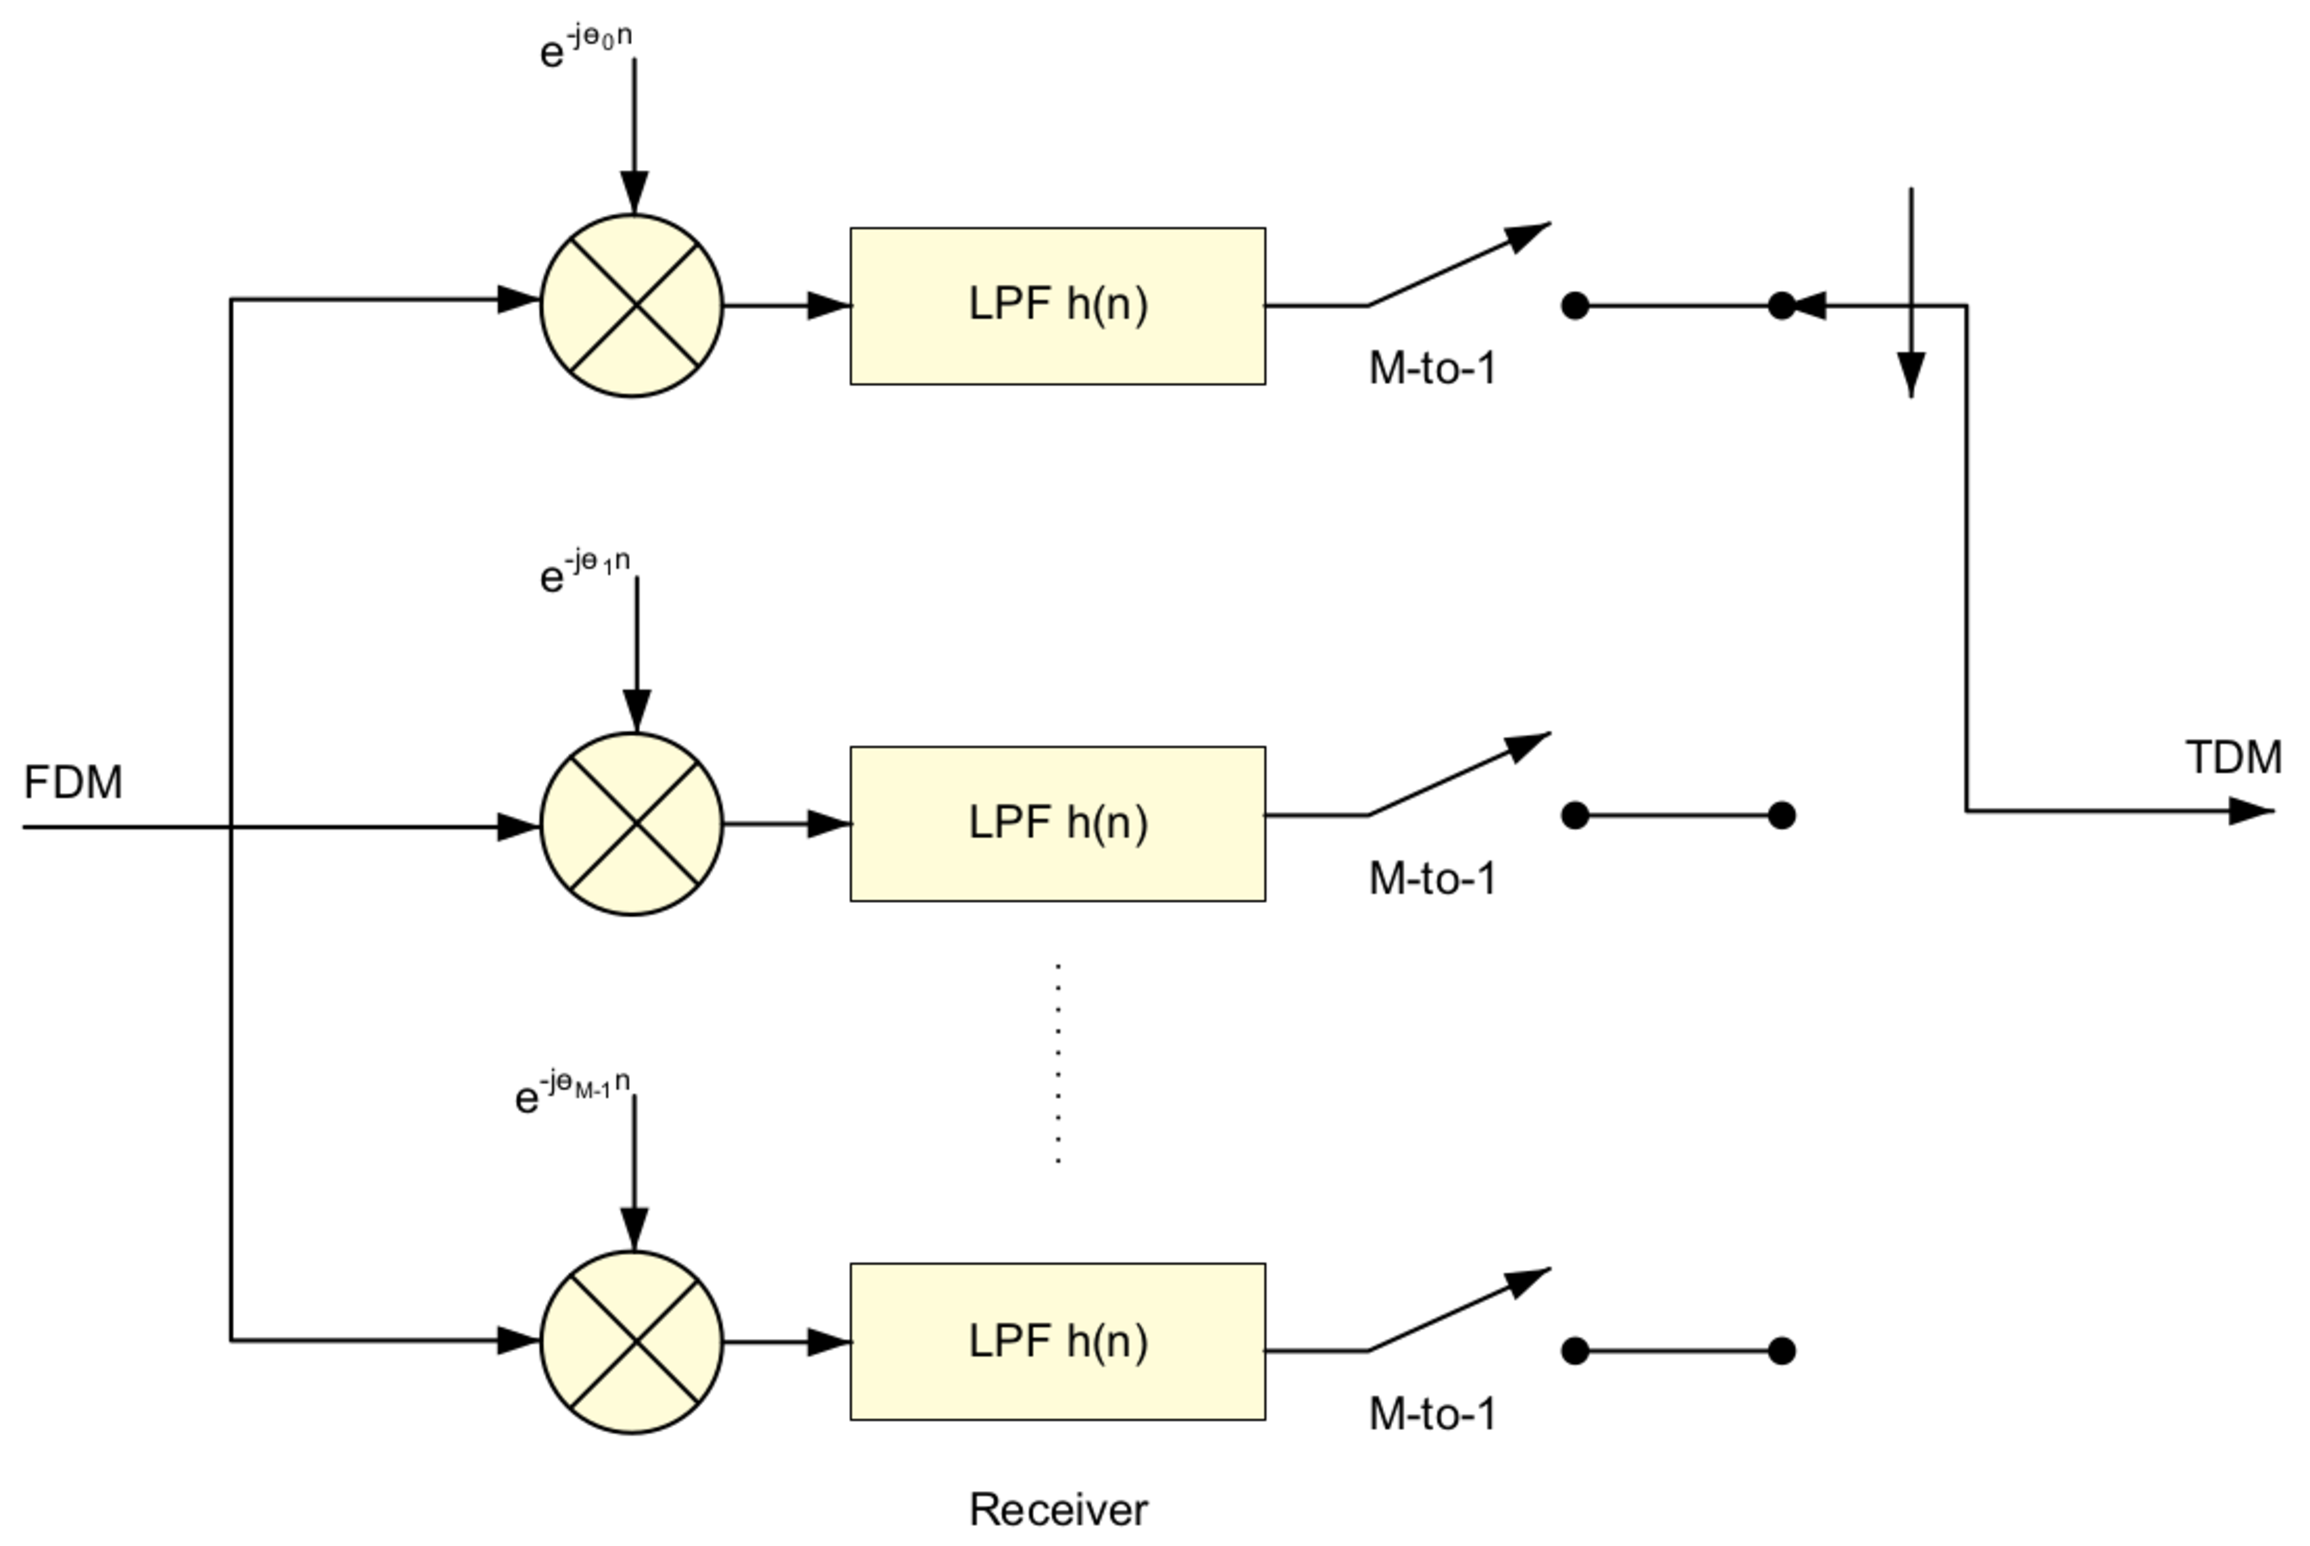
\includegraphics[width=1.09\textwidth]{Rx_channelizer}}
												\only<2>{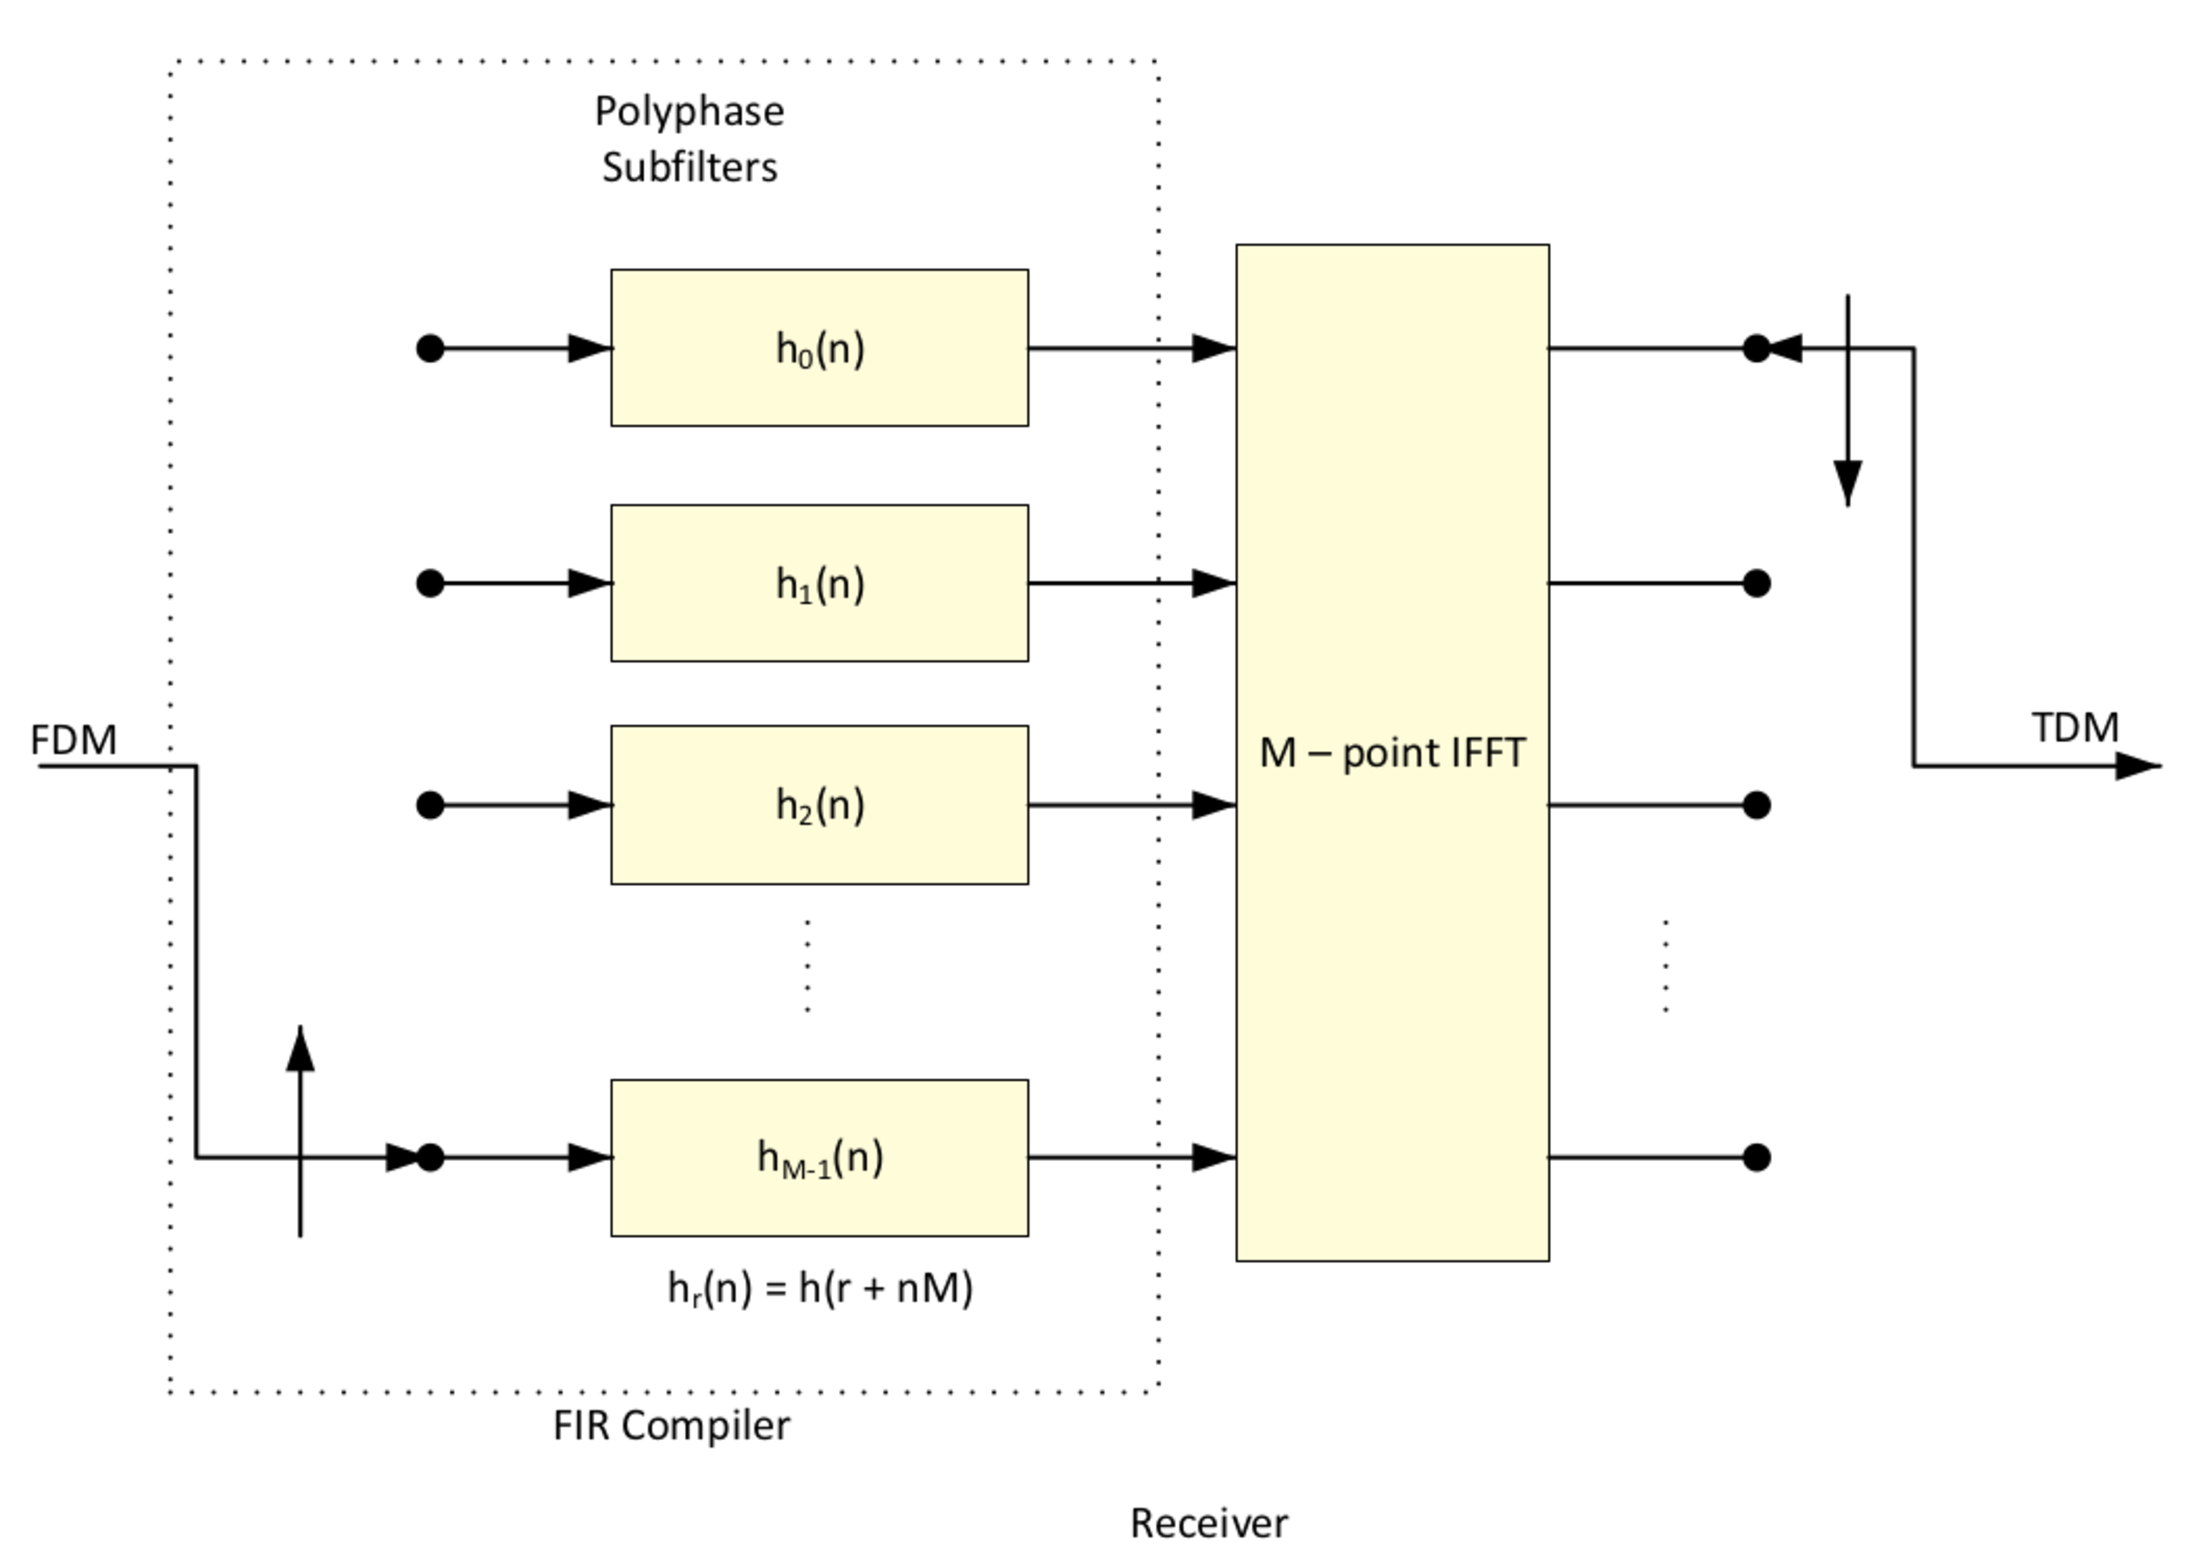
\includegraphics[width=1.09\textwidth]{Rx_channelizer_con_IFFT}}
								\end{column}
				\end{columns}
\end{frame}

%\begin{frame}{Channelizer Rx}
%				\begin{center}
%								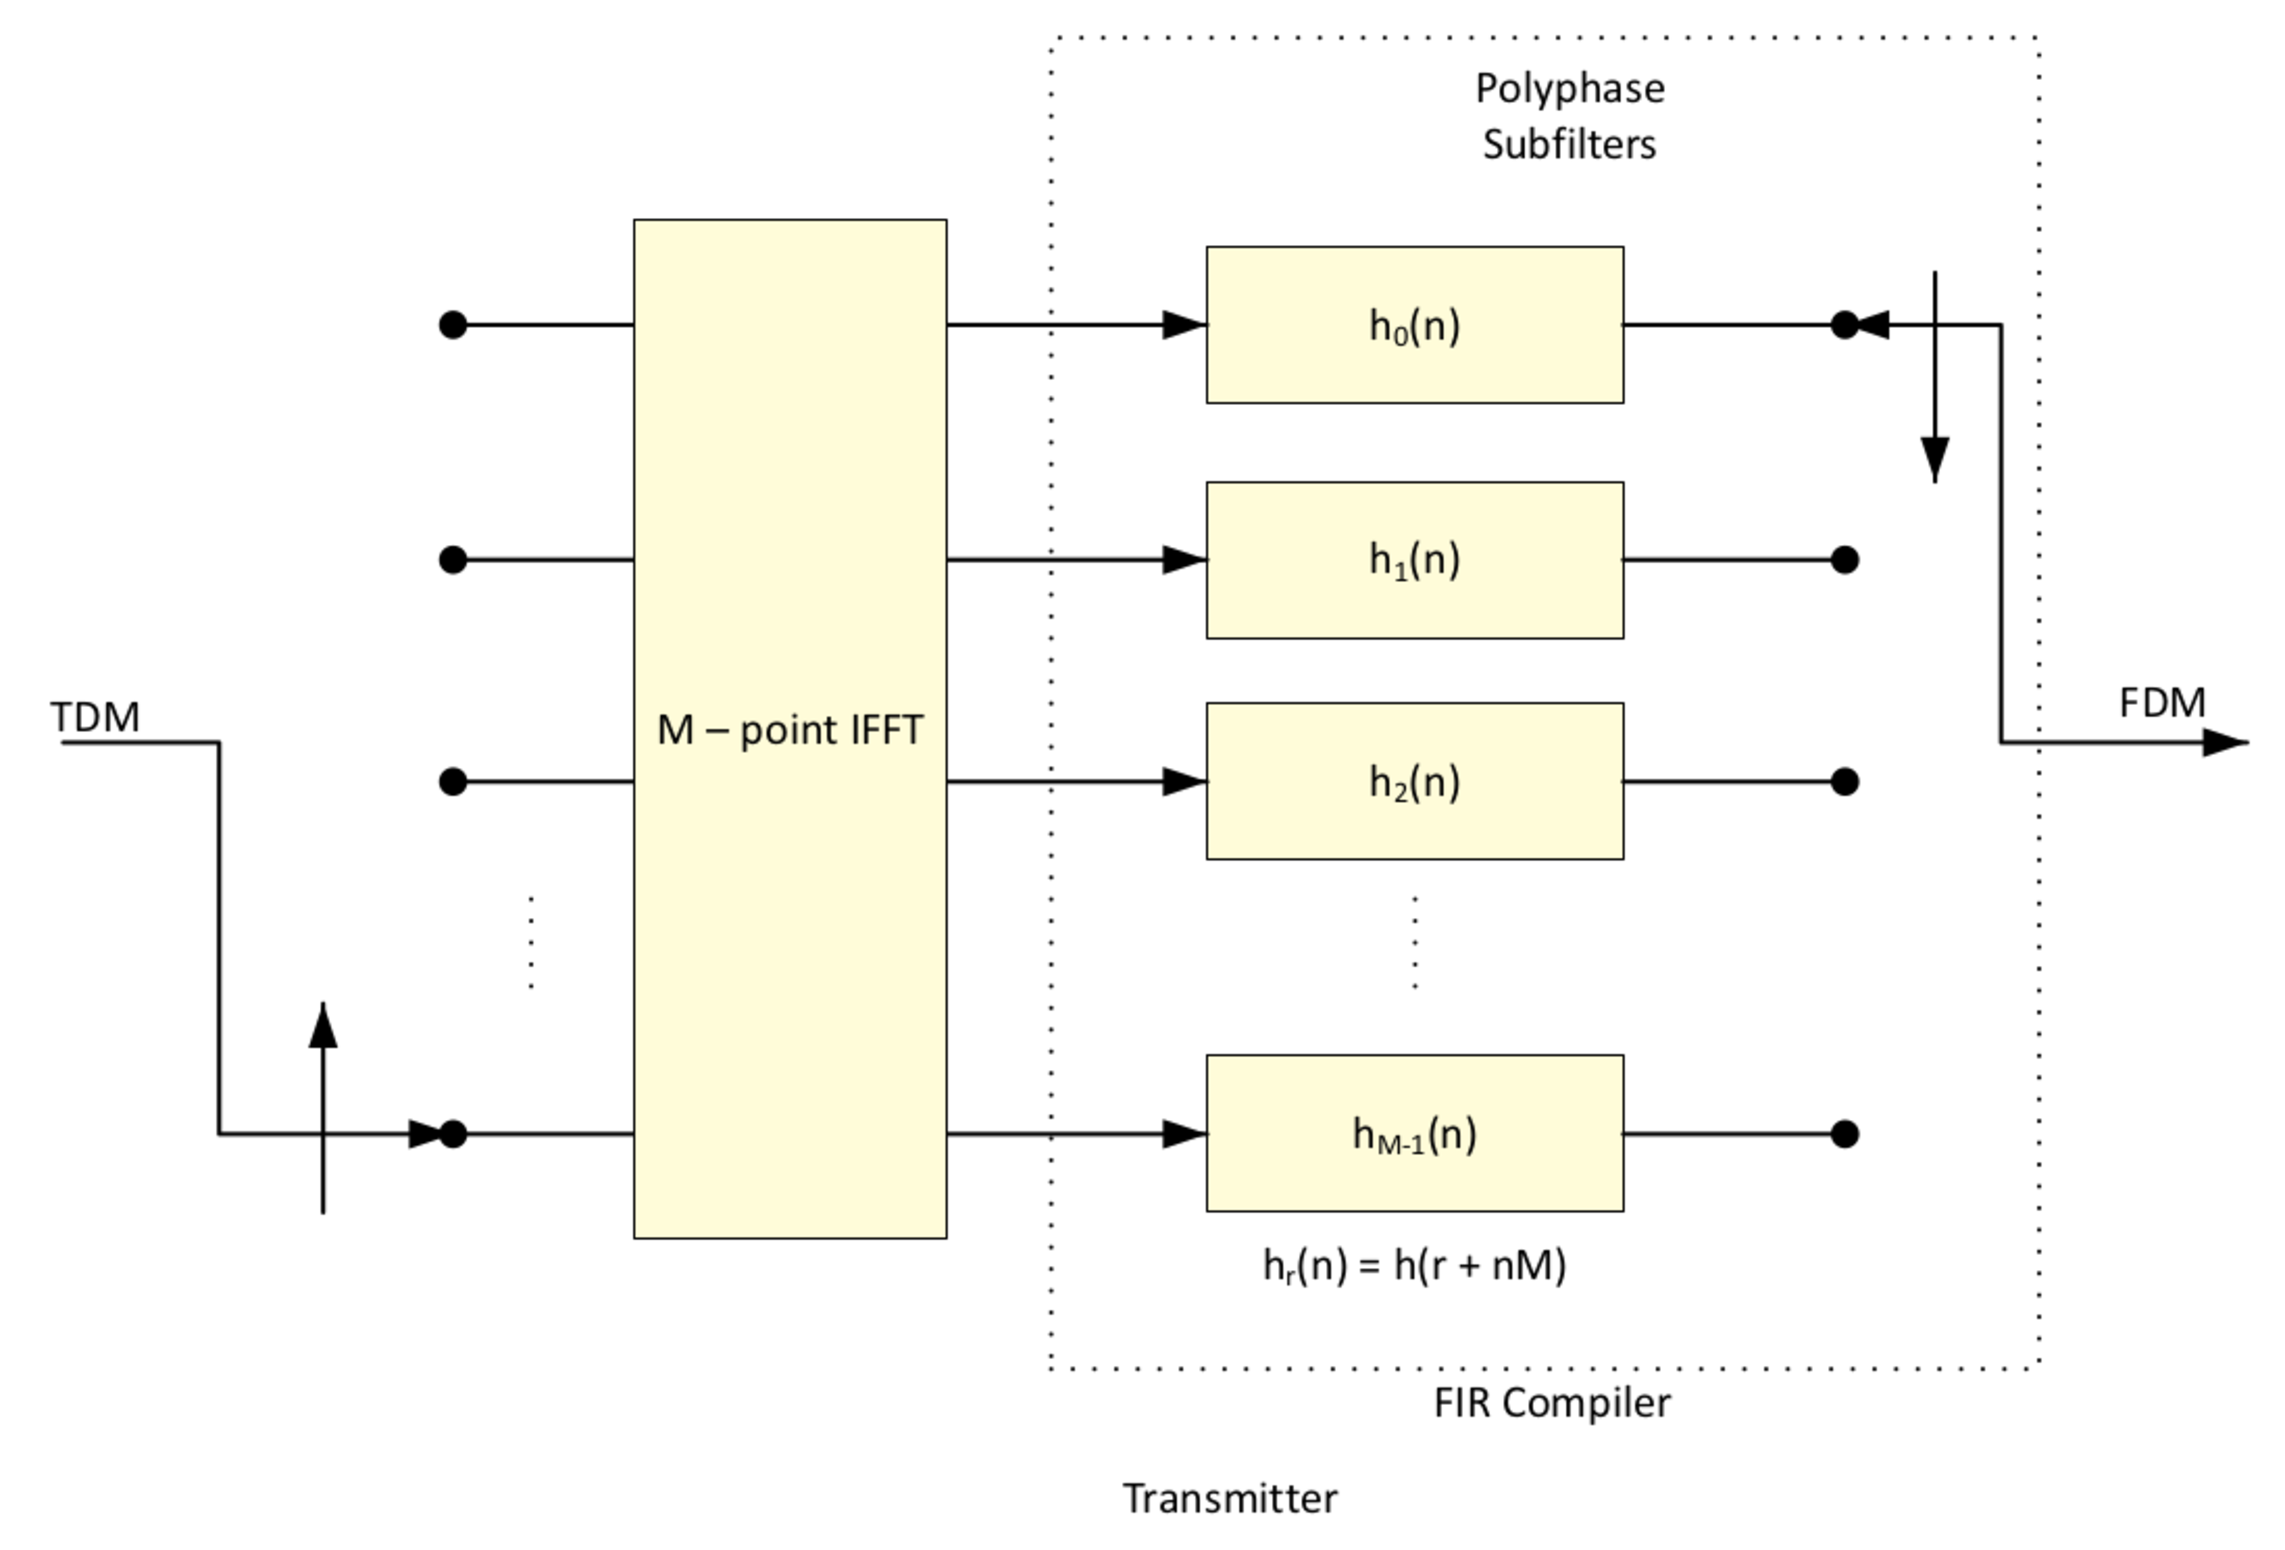
\includegraphics[width=0.8\textwidth]{Tx_channelizer_con_IFFT}
%								\only<2>{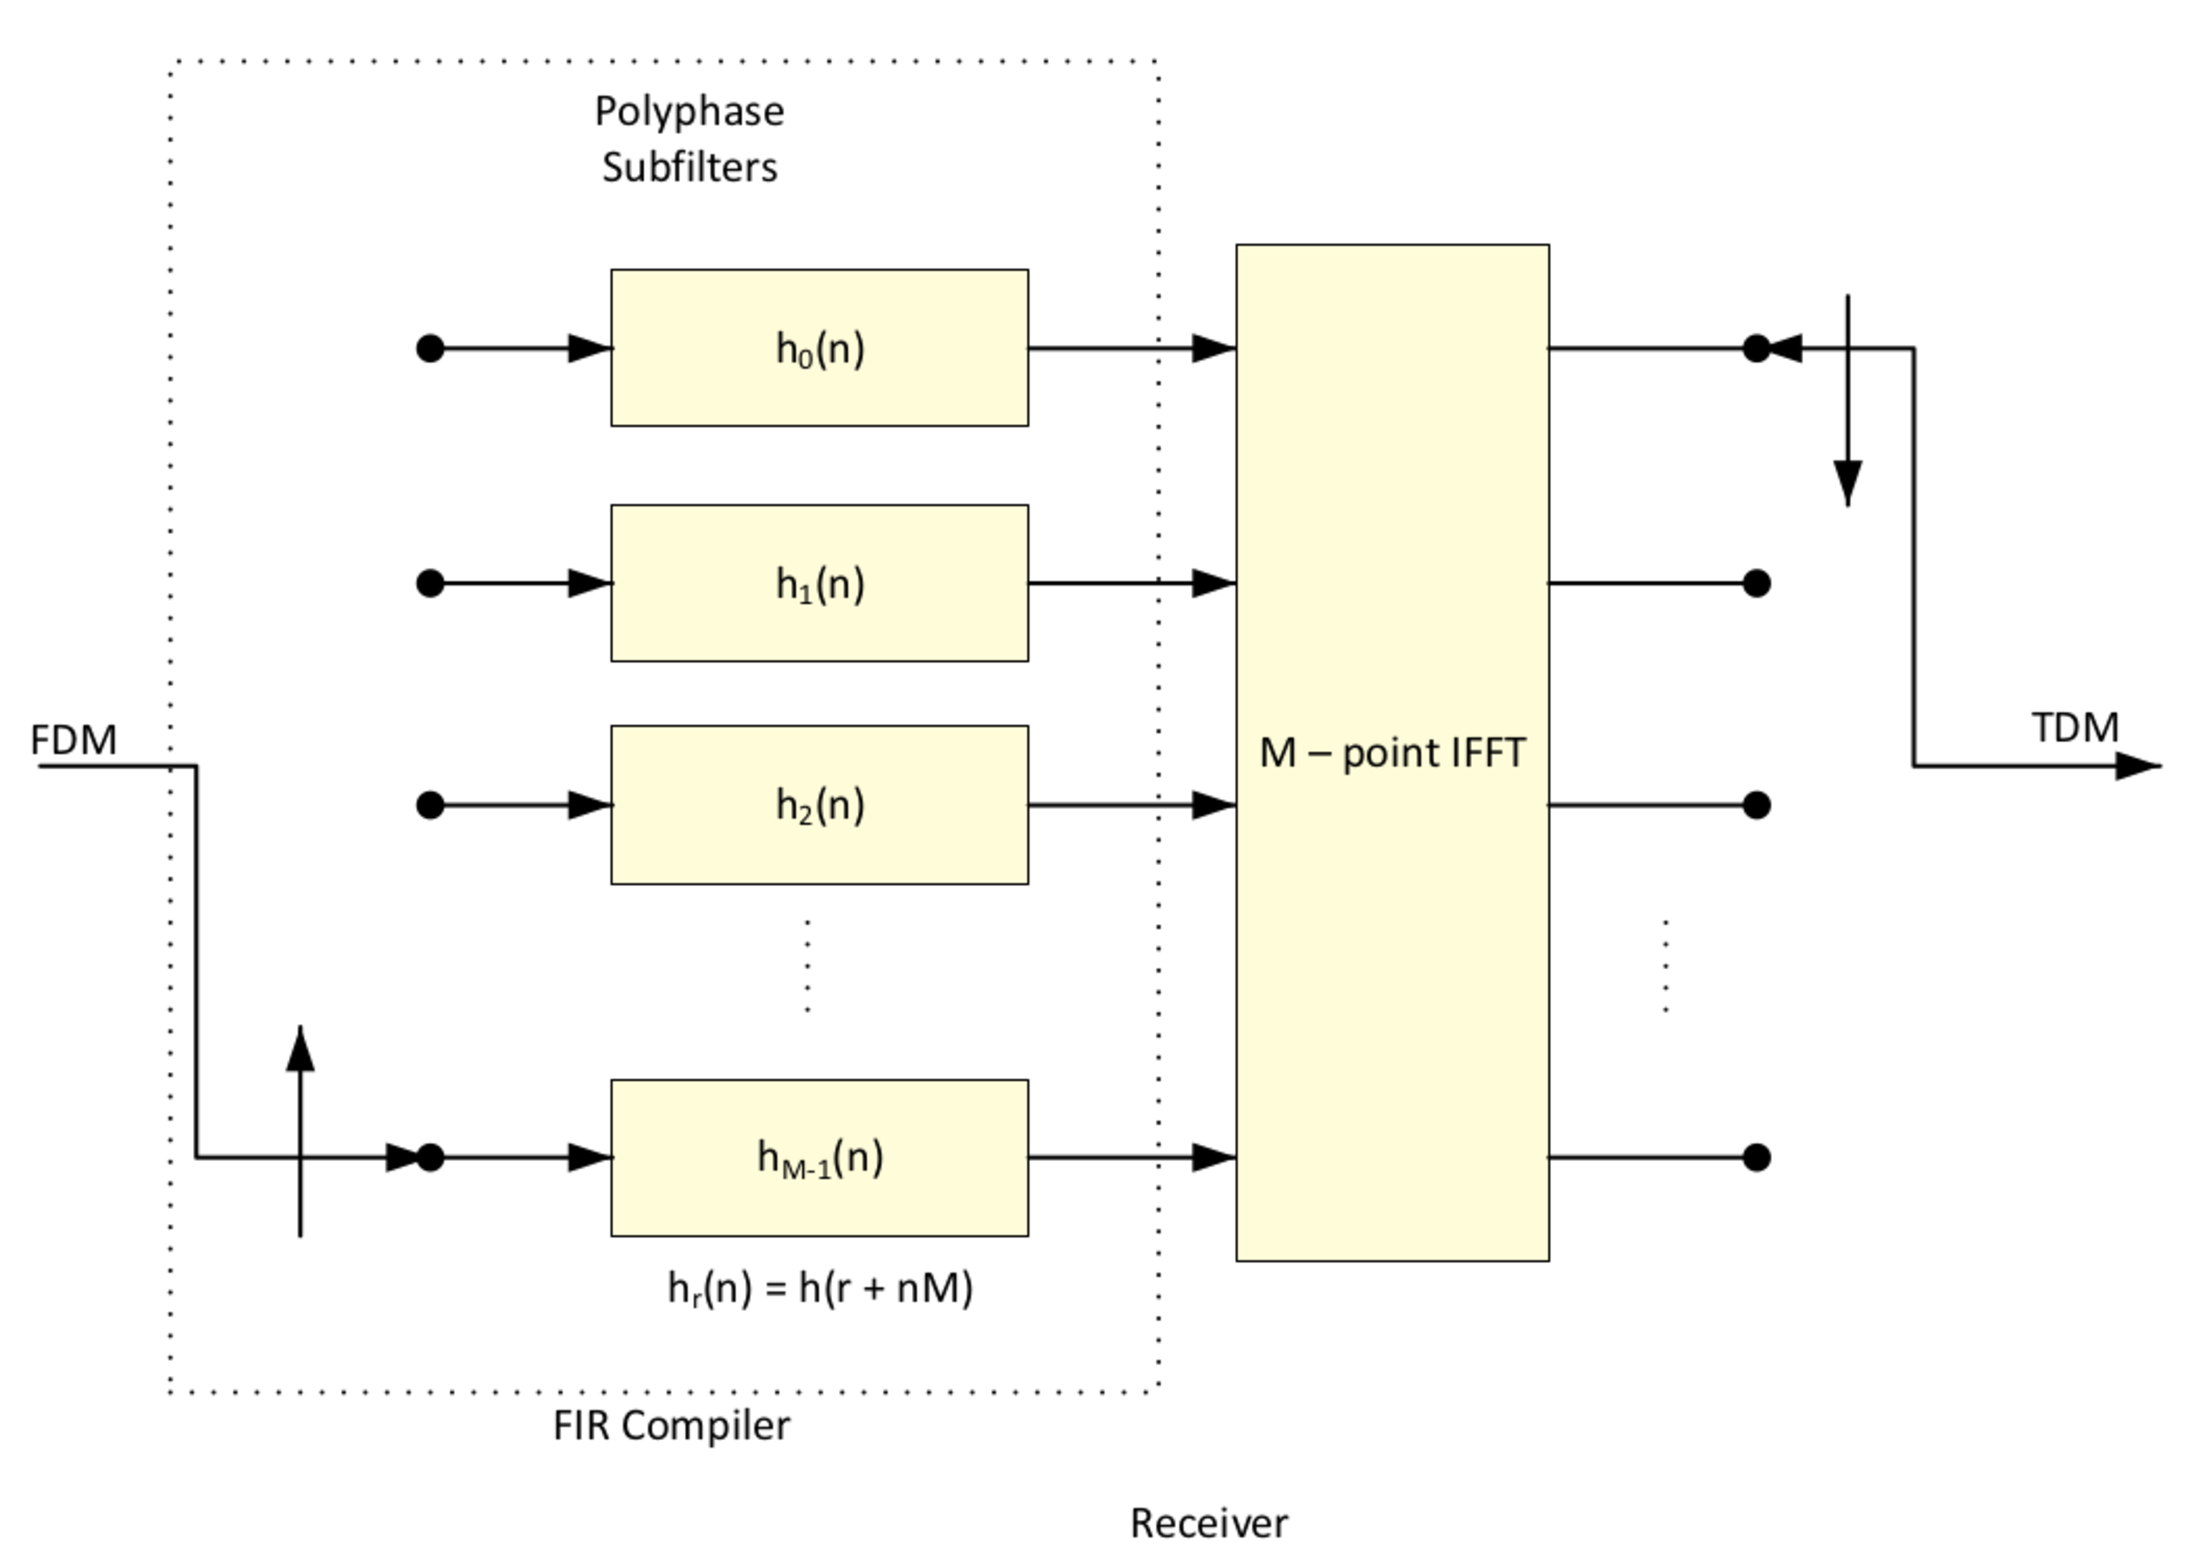
\includegraphics[width=0.8\textwidth]{Rx_channelizer_con_IFFT}}
%				\end{center}
%\end{frame}

\begin{frame}{PFB operación básica (D=M), Rx}
				\begin{center}
								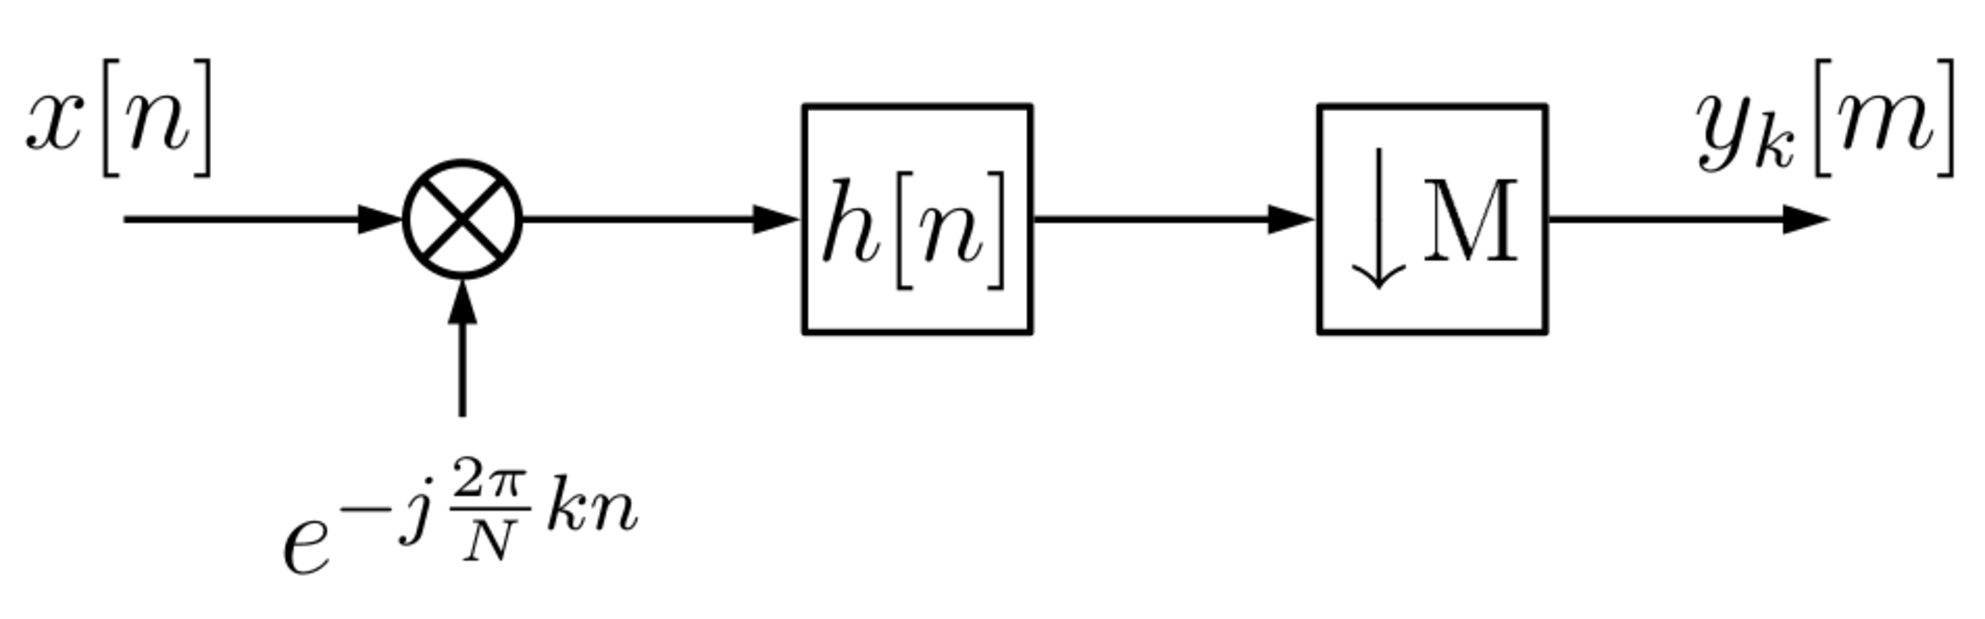
\includegraphics[width=0.6\textwidth]{PFB_basic_operation}
				\end{center}
				\begin{columns}
								\begin{column}{0.5\textwidth}{{\color{olive}Estructura polifase}}
												\footnotesize{
																\\Secuencia de entrada para cada canal $k$:
																\begin{equation*}\label{eq:xk_decimated}
																				x_k(n) = x(nM + k), \quad k = 0,1,..., M-1
																\end{equation*}
																Respuesta al impulso:
												\begin{equation*}\label{eq:pk_filter}
																p_k(n) = h_0(nM - k), \quad k = 0,1, ...,M-1
												\end{equation*}}
								\end{column}
								\begin{column}{0.5\textwidth}{}

												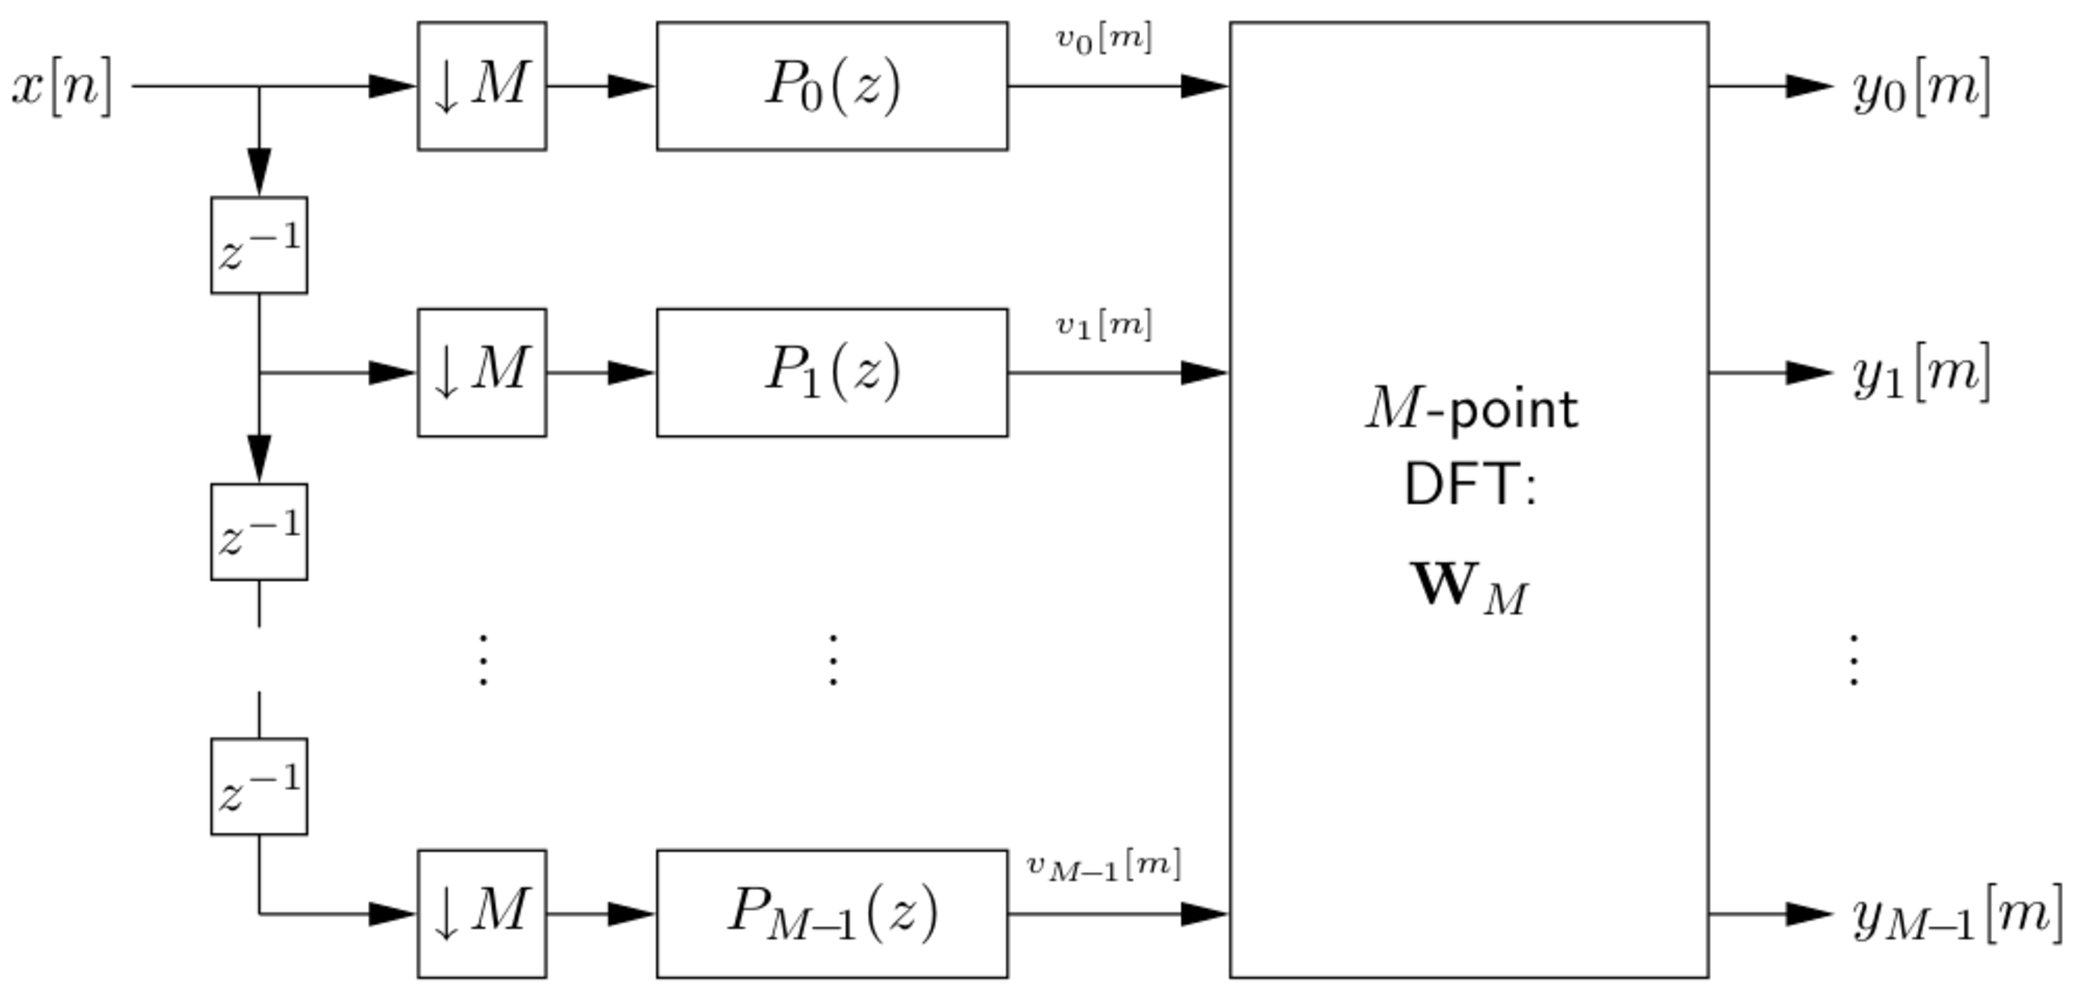
\includegraphics[width=1.1\textwidth]{uniform_PFB}
								\end{column}
				\end{columns}
								\alert{\begin{equation*}\label{eq:fft_out}
												Y_k(m) = \sum_{r=0}^{M-1}\Big[ \sum_l p_r(l) x_r(m-l)\Big] e^{-j2\pi
												rk/M}, \quad k = 0,1,...,M-1.
								\end{equation*}}

\end{frame}

				\section{Filtro prototipo}
				\begin{frame}{Filtro prototipo (M canales)}
								\begin{equation*}\label{eq:pf_filter}
												H_k(w) = H_0\Big(w-\frac{2\pi k}{M}\Big),   \quad k = 1,2,...,M-1.
								\end{equation*}
								\begin{columns}
												\begin{column}{0.5\textwidth}
																\only<1>{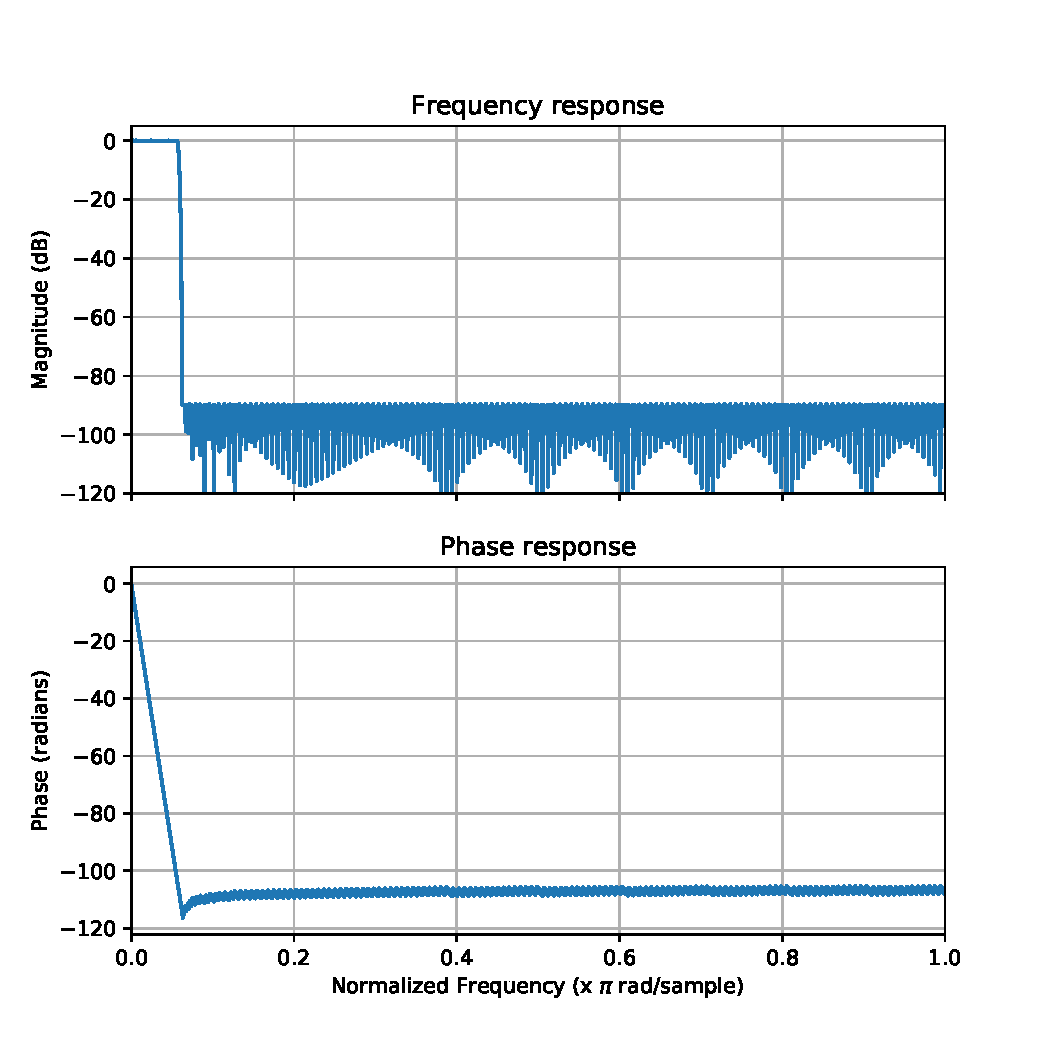
\includegraphics[width=1.2\textwidth]{prototipo}}
																\only<2>{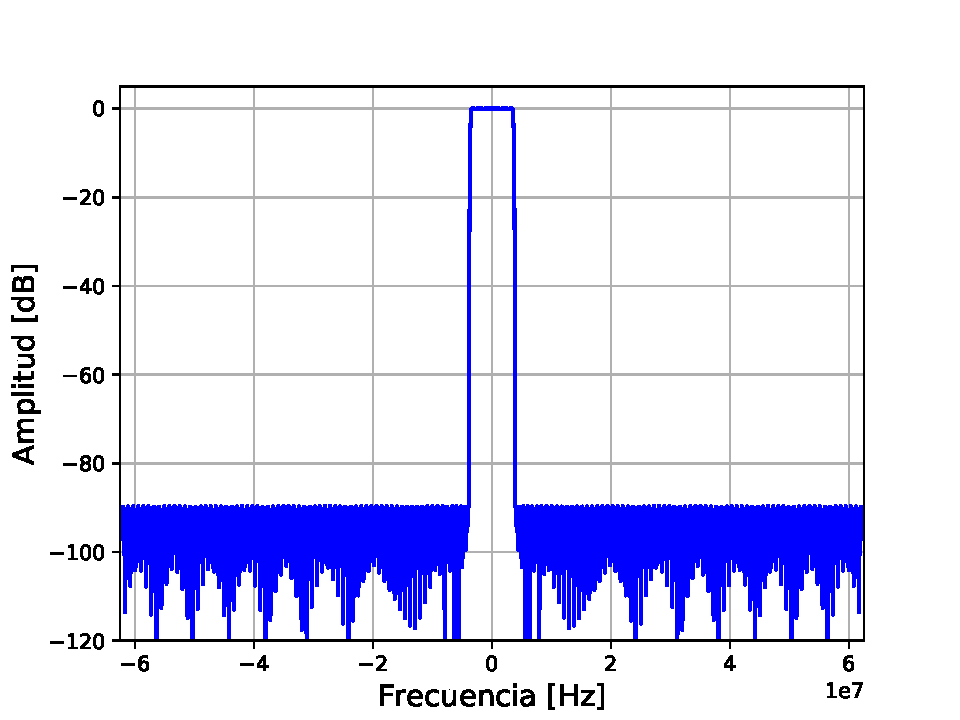
\includegraphics[width=1.15\textwidth]{one_filter_spectrum}}
												\end{column}
												\begin{column}{0.5\textwidth}
																\only<1>{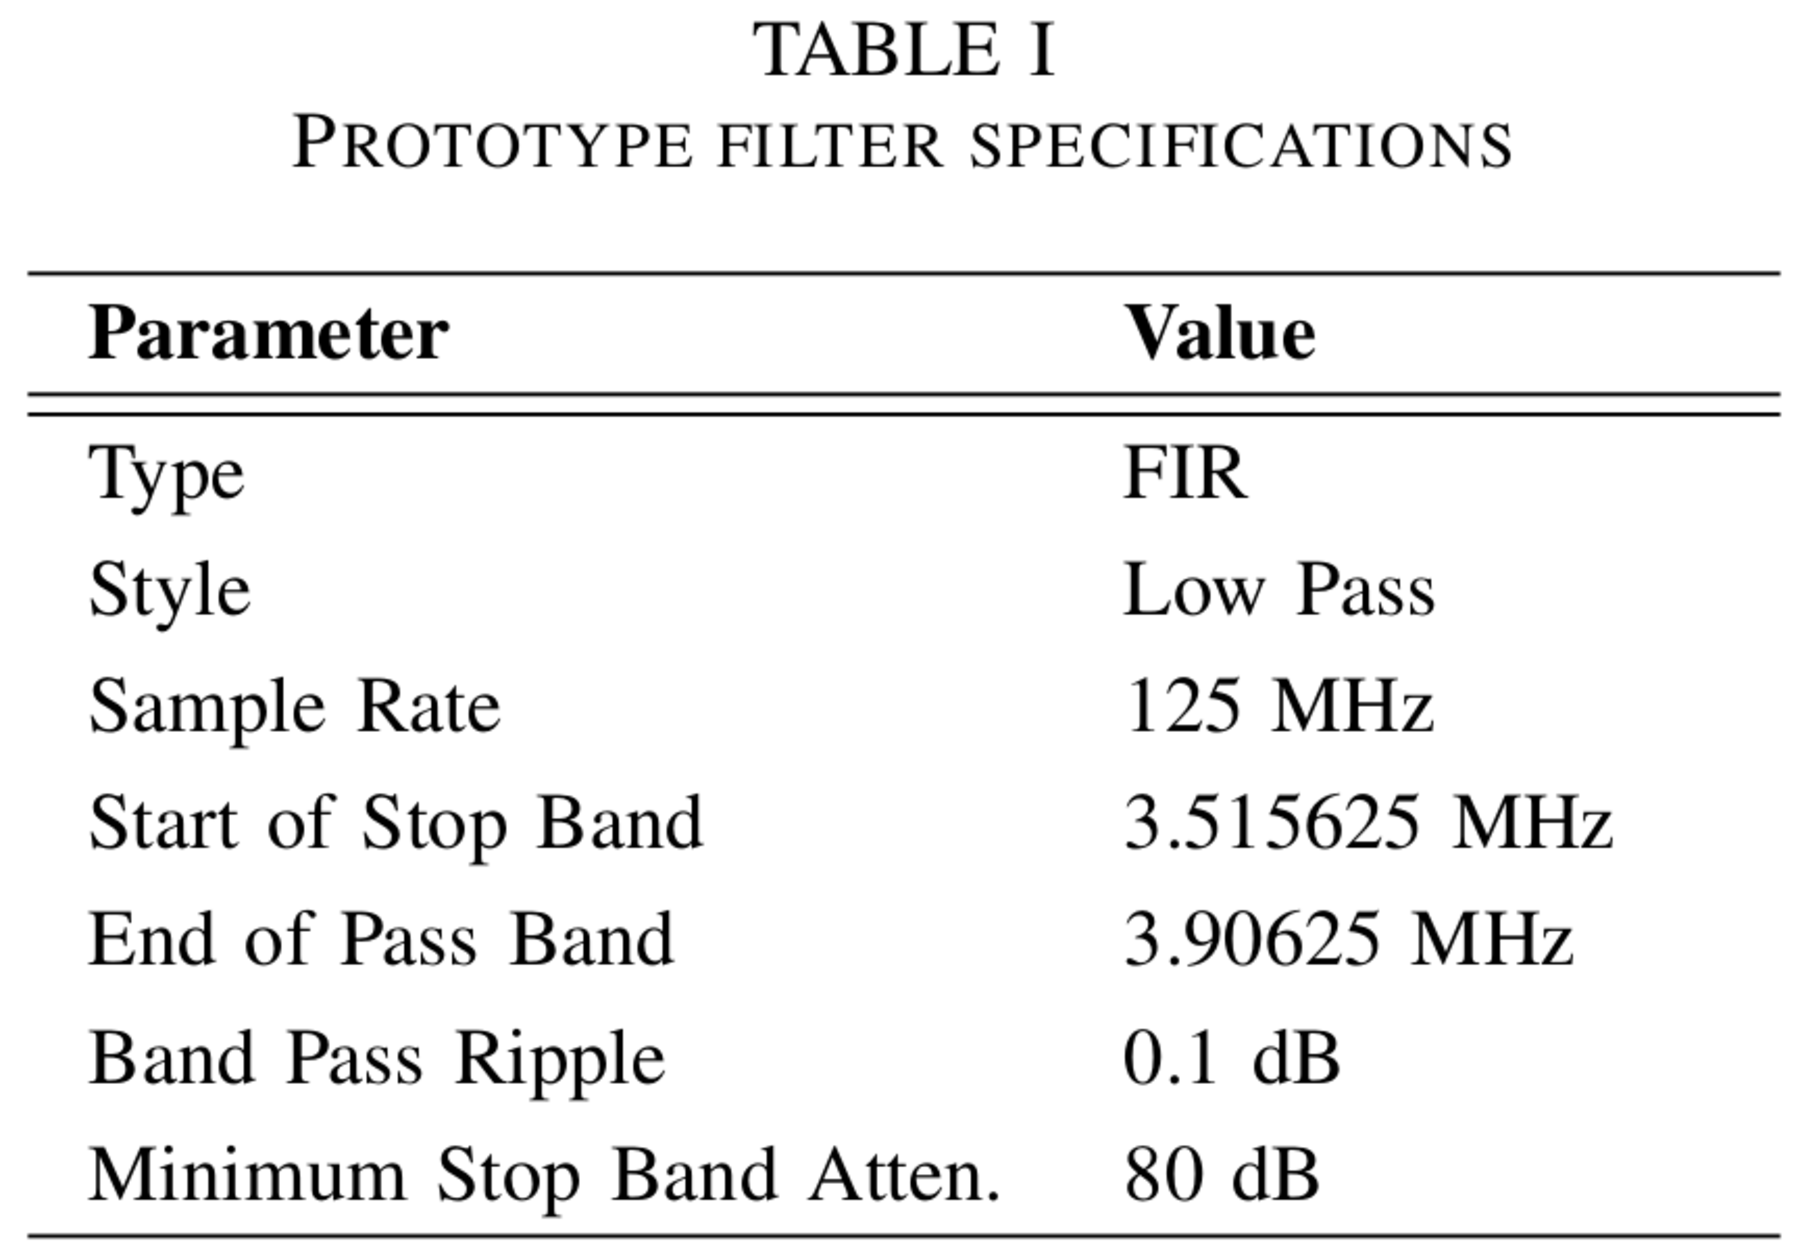
\includegraphics[width=0.8\textwidth]{prototipo_specifications_table}}
																\only<2>{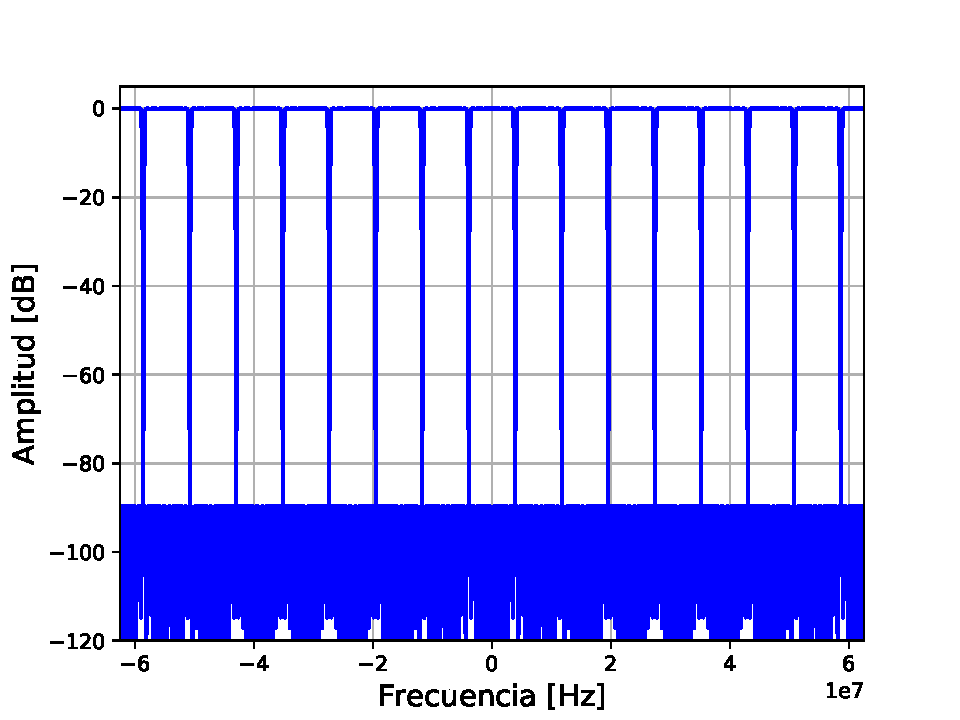
\includegraphics[width=1.15\textwidth]{full_spectrum}}
												\end{column}
								\end{columns}
				\end{frame}

				%\section{El algoritmo de Goertzel}
				%\begin{frame}{El algoritmo de Goertzel}
				%				\begin{itemize}
				%								\item Finalize performance requirements for firmware 
				%								\item Finalize performance requirements for Tx and Rx parts 
				%								\item First tests of RxChannelizer (front-end, mixers, filters,
				%												DC-block, etc.)
				%				\end{itemize}
				%								\centering
				%								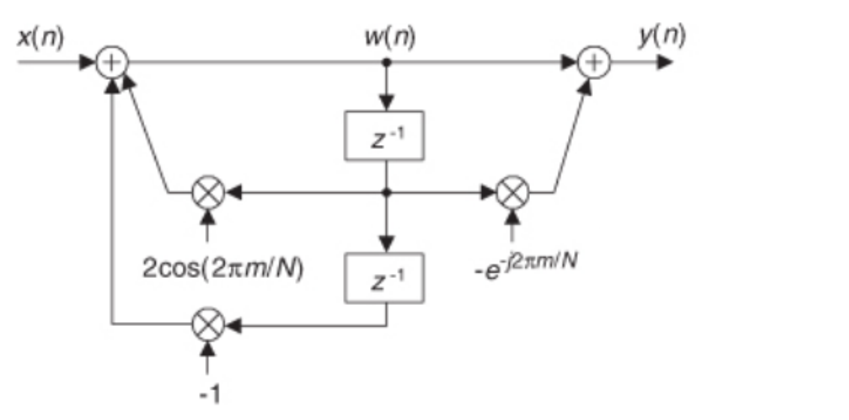
\includegraphics[width=0.45\textwidth]{goertzel_algo}
				%\end{frame}
				%
				%\begin{frame}{El algoritmo de Goertzel}
				%				\begin{itemize}
				%								\item Finalize performance requirements for firmware 
				%								\item Finalize performance requirements for Tx and Rx parts 
				%								\item First tests of RxChannelizer (front-end, mixers, filters,
				%												DC-block, etc.)
				%				\end{itemize}
				%								\centering
				%								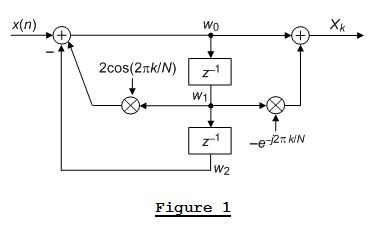
\includegraphics[width=0.45\textwidth]{goertzel_non_integer_figure1}
				%\end{frame}
				%
				%------------------------------------------------------------------------------
\section{Simulaciones y pruebas}
\begin{frame}{Implementación en Vivado}
				\frametitle{Canalizador de 16 canales}
												\begin{tikzpicture}
																\node<1>[anchor=north west,inner sep=0]
																at (0,8)
																{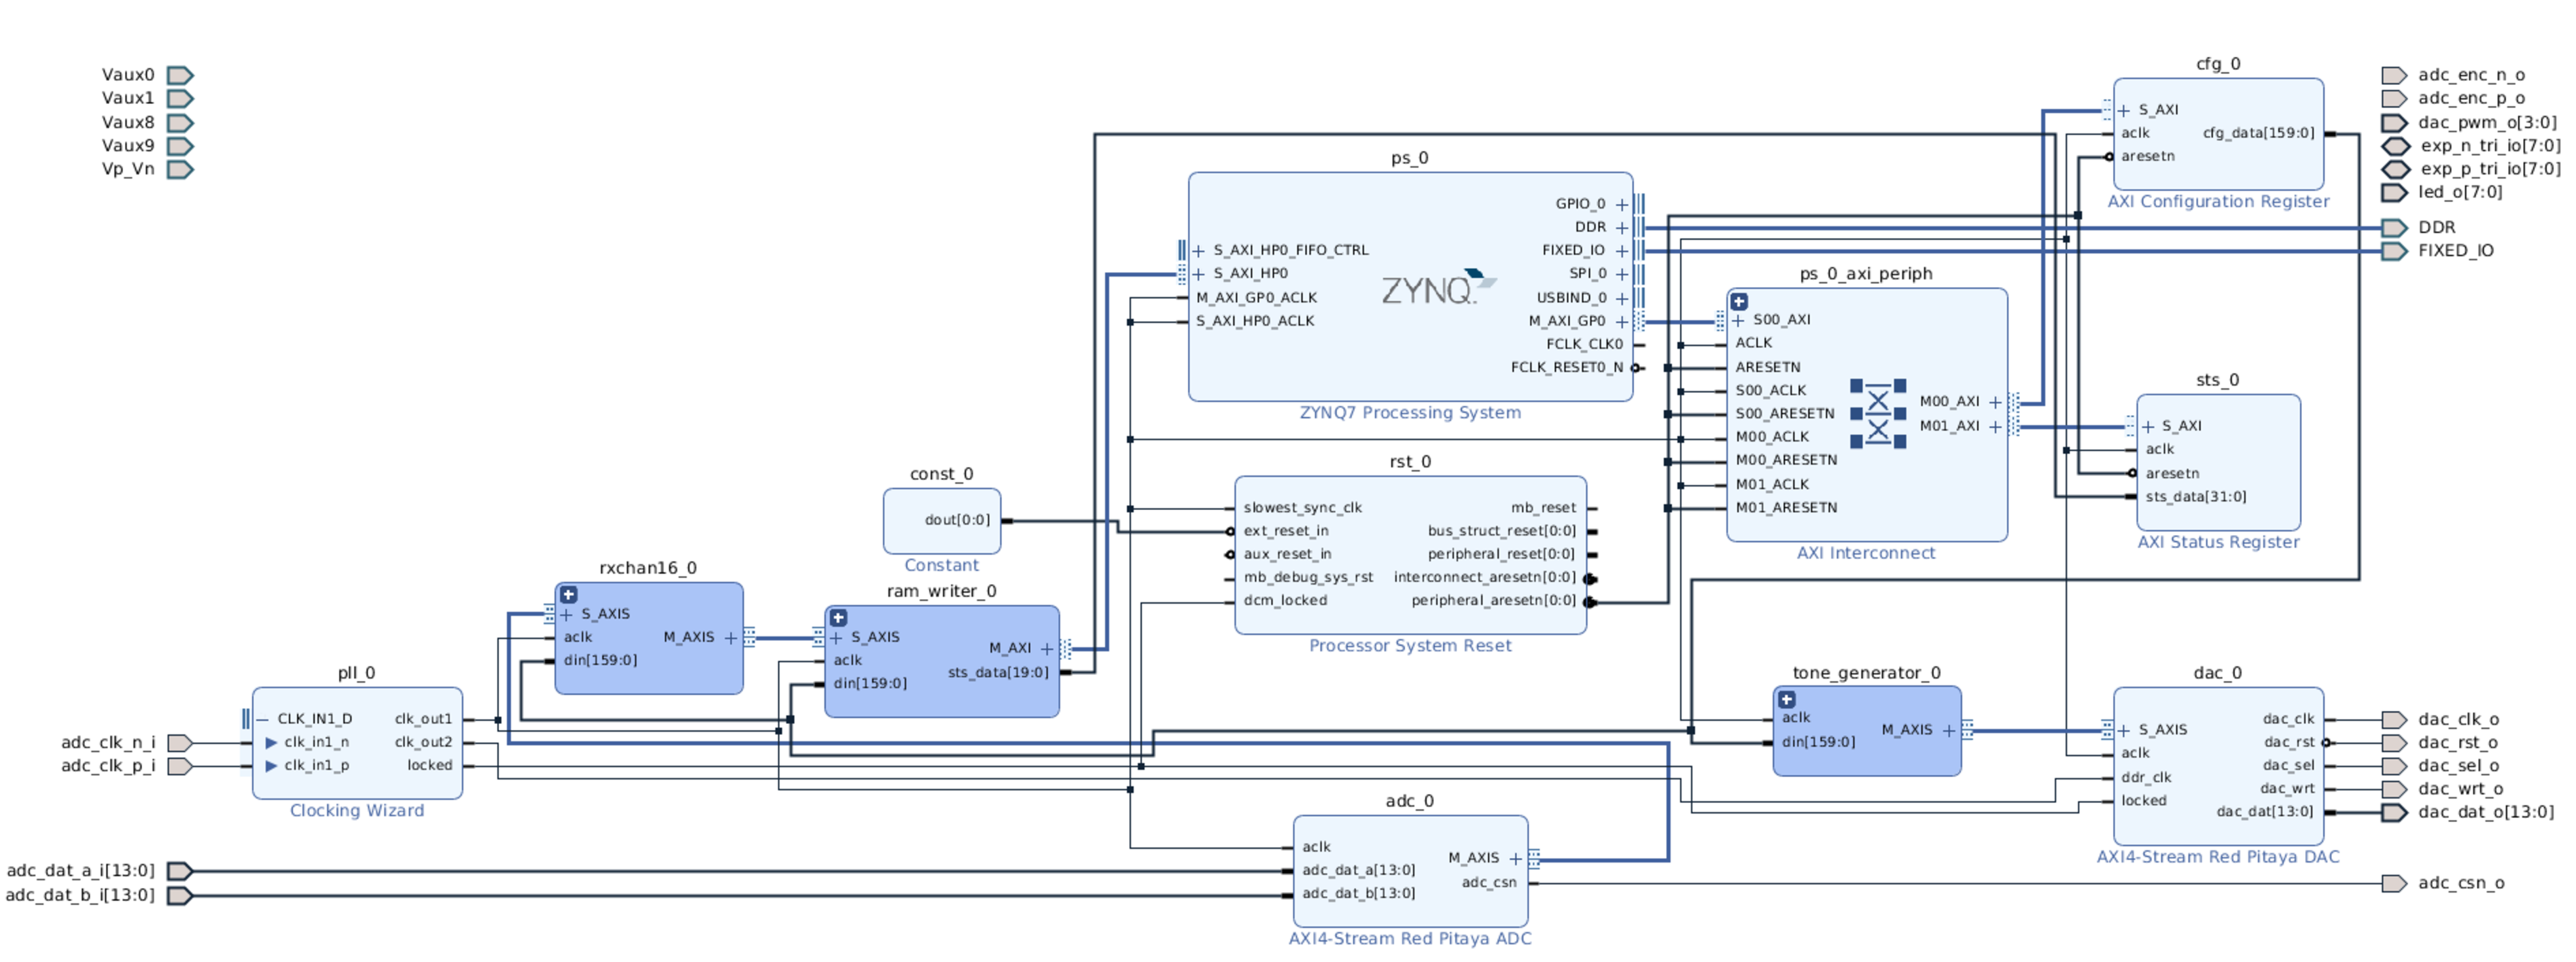
\includegraphics[width=1.05\textwidth]{esquema_rxch16_vivado}};
																\node<2>[anchor=north west,inner sep=0]
																at (0,8)
																{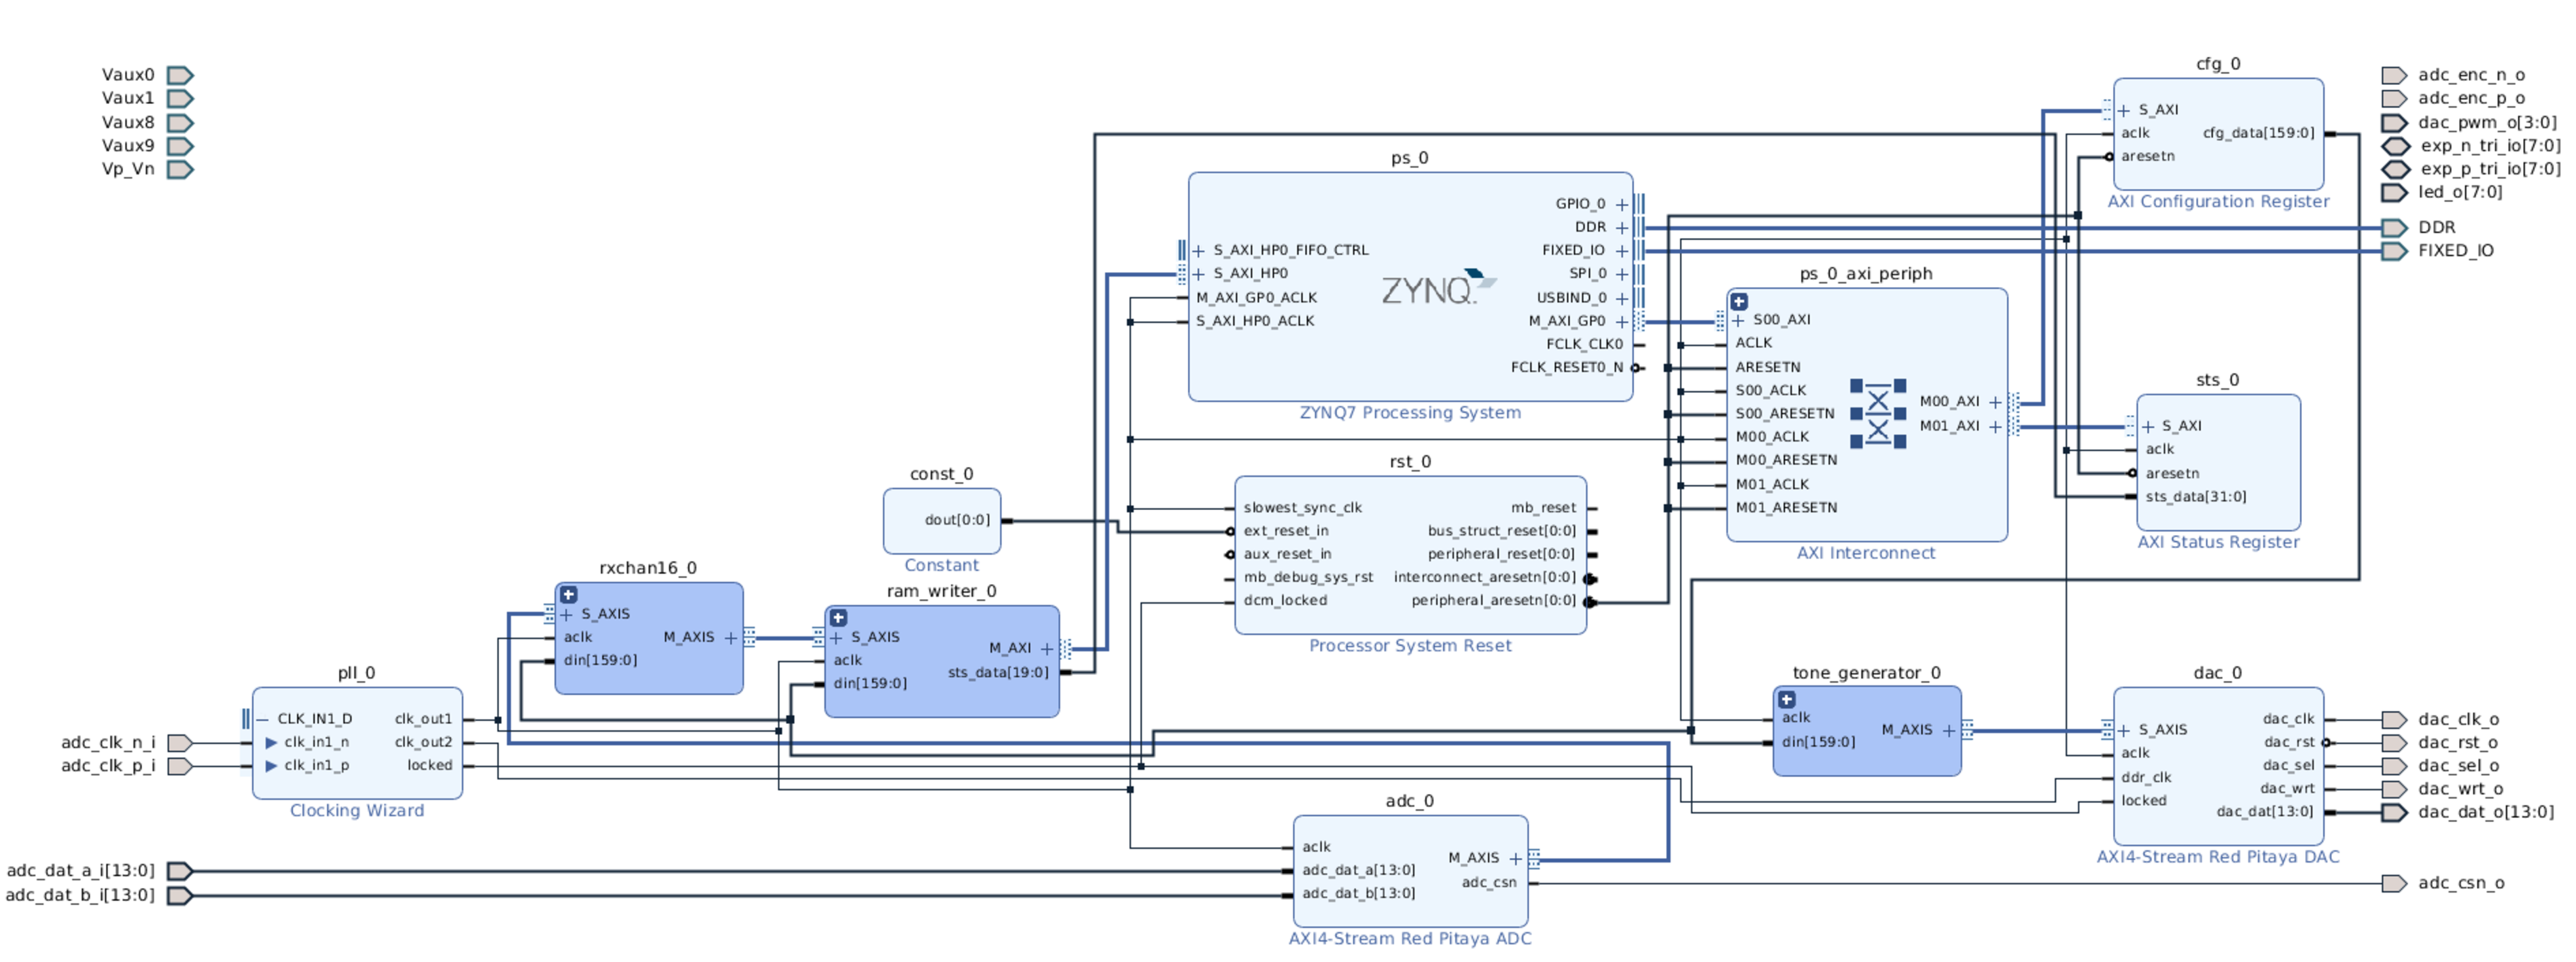
\includegraphics[width=0.8\textwidth]{esquema_rxch16_vivado}};
																\draw<2>[red,ultra thick,rounded corners]
																(2.0,5.0) rectangle (3.2,5.9);
																\node<2>[anchor=south west,inner sep=0] at
																(0,0){\fbox{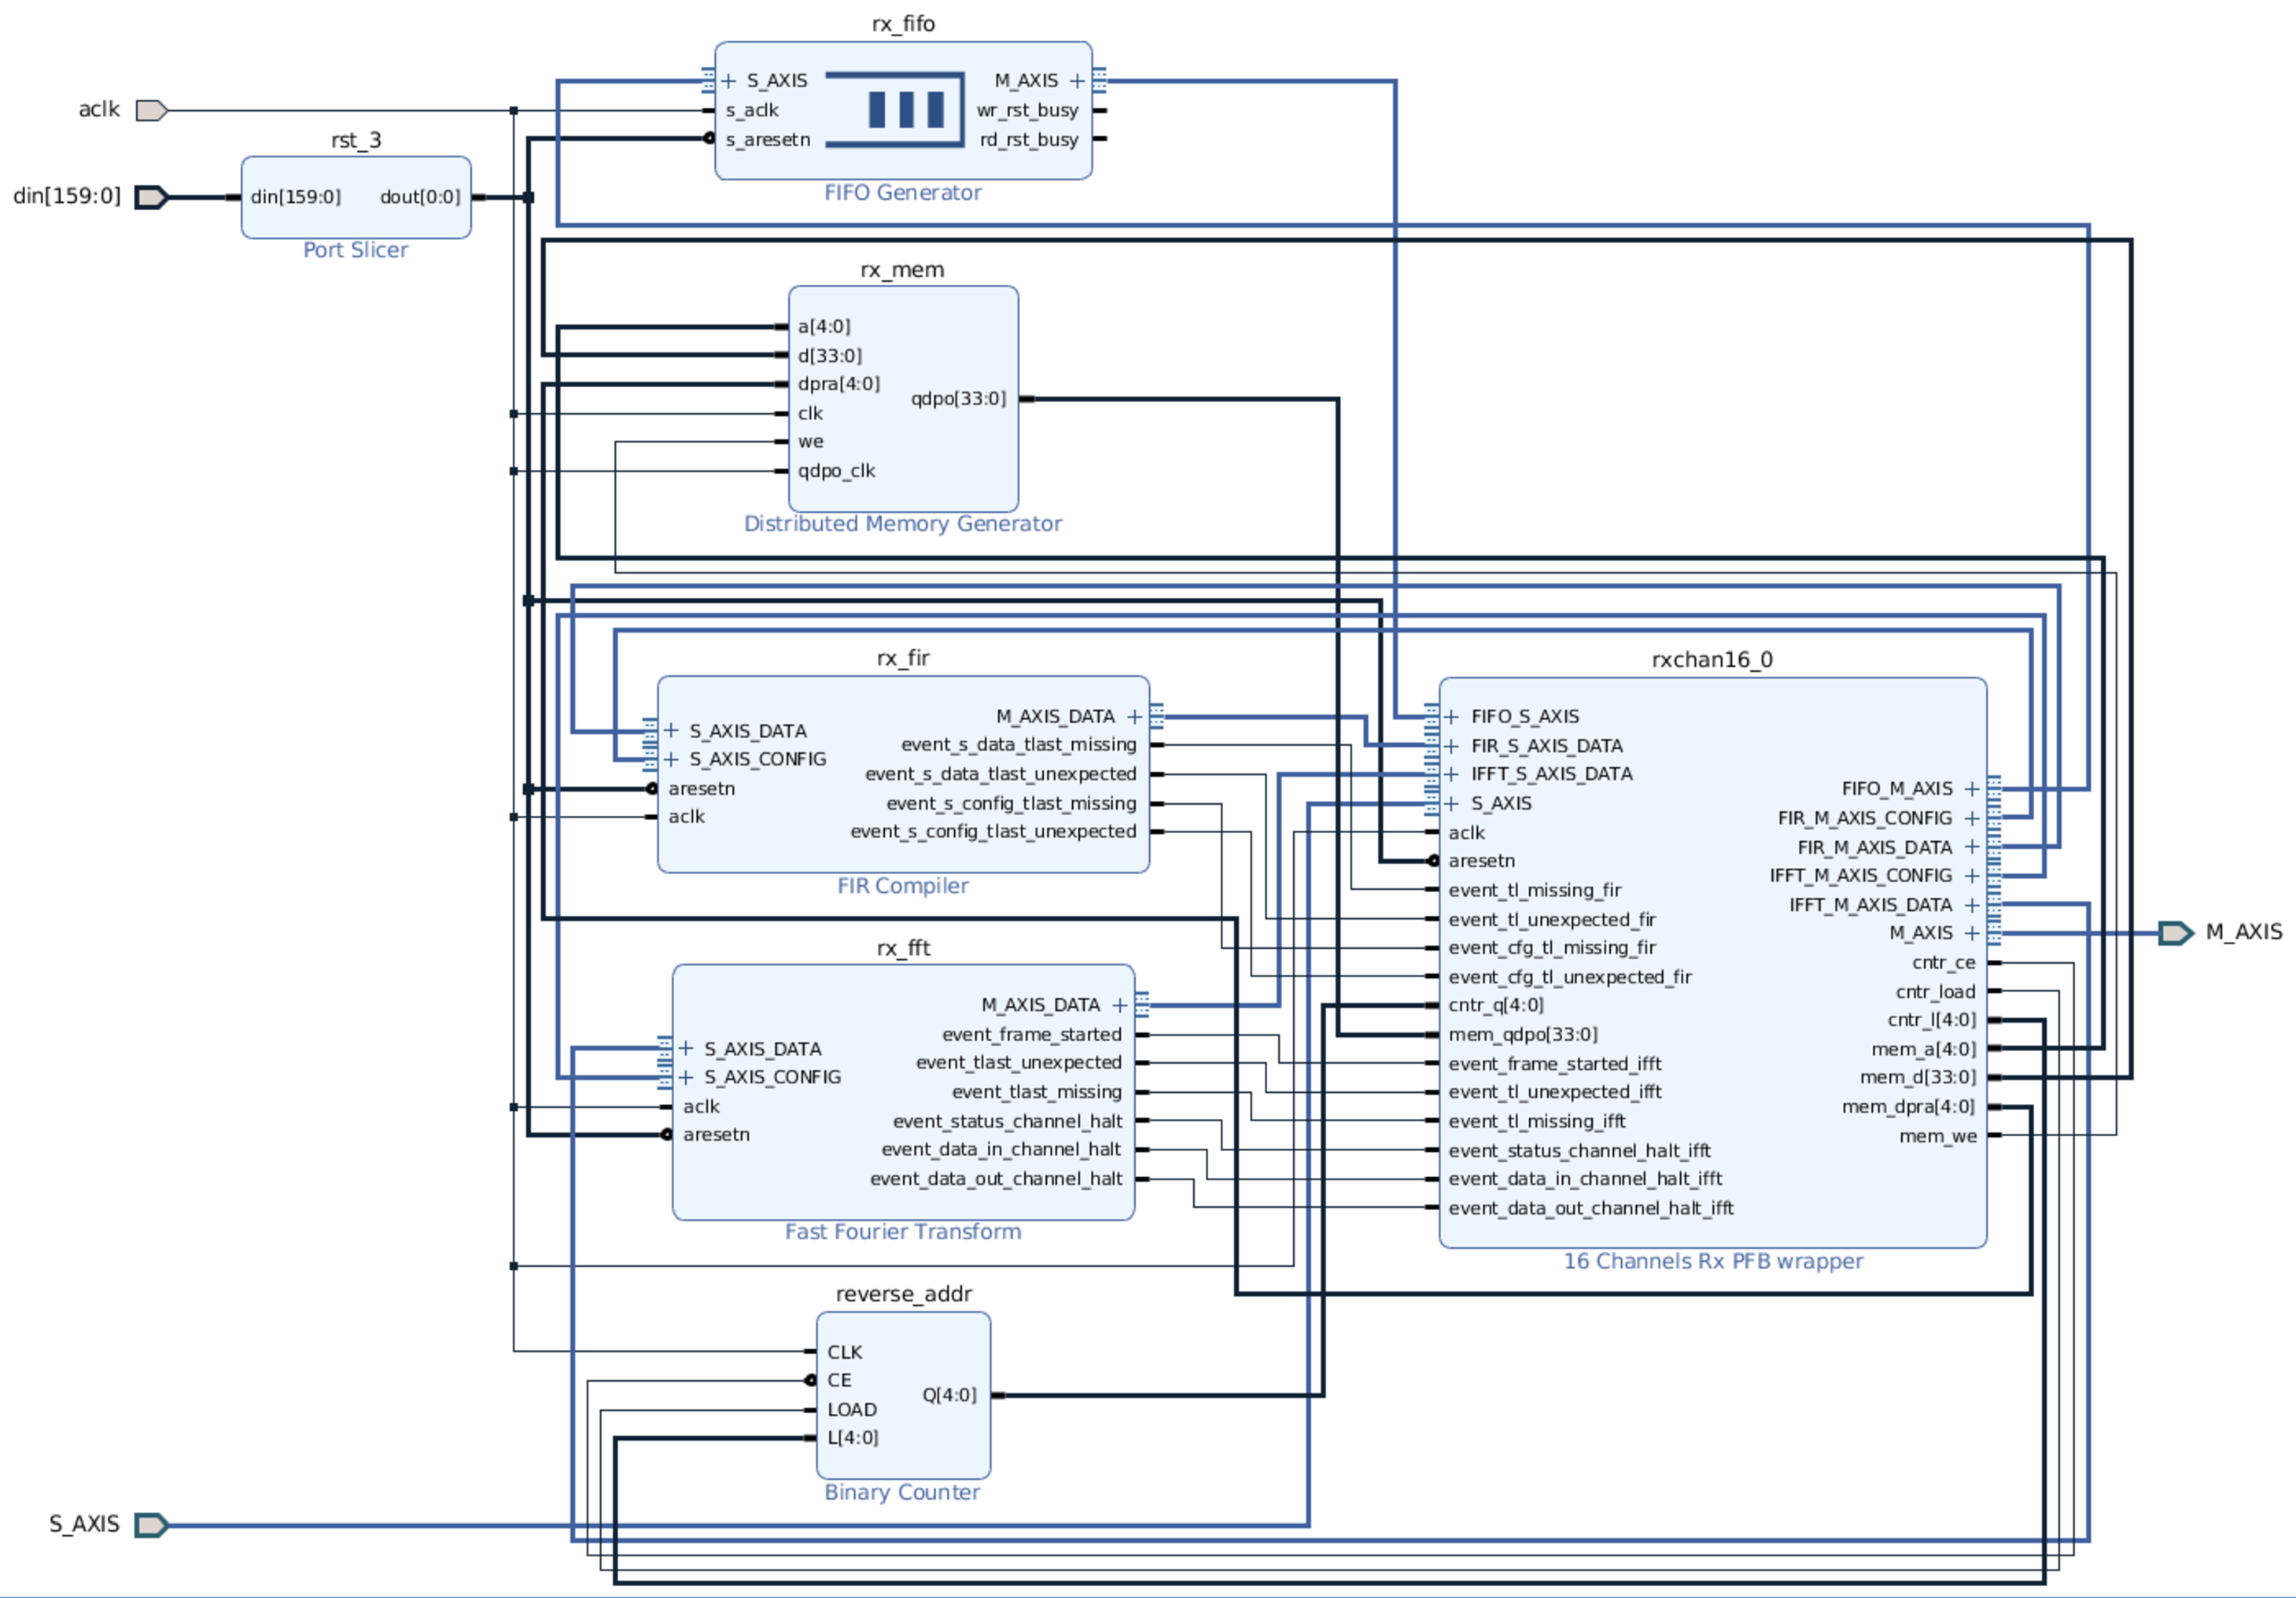
\includegraphics[width=.5\textwidth]{rxch16_vivado}}};
																%\only<3>{\node[anchor=north west,inner sep=0] at
																%(5,5){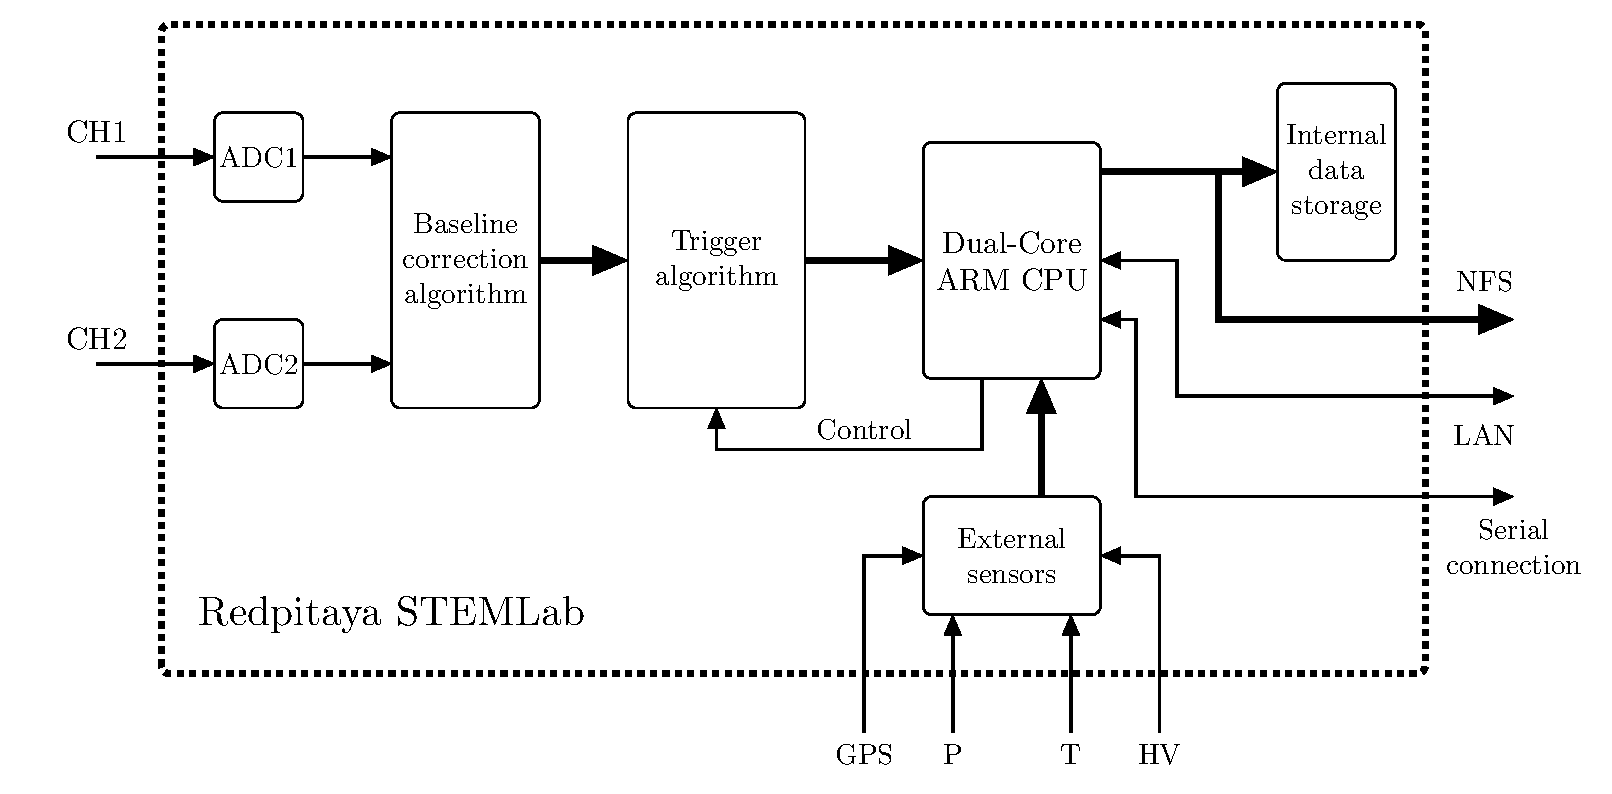
\includegraphics[width=\textwidth]{diag_sys}};}
												\end{tikzpicture}
\end{frame}

\begin{frame}{Implementación en Vivado}
				\frametitle{Reportes de utilización. Comparación de implementaciones}
				Cambios en la configuración del filtro polifásico FIR (7.5\% vs. 87.5\%
				de DSP Slices)

				\begin{columns}
								\begin{column}{0.5\textwidth}{{\color{blue}Versión ``lenta''}}
												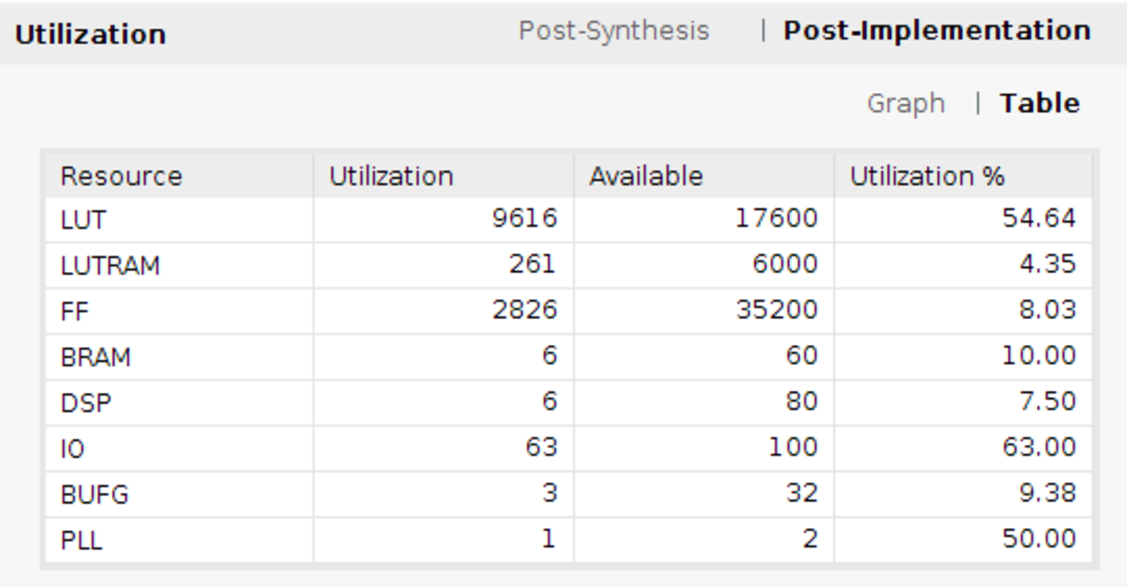
\includegraphics[width=\textwidth]{utilization_table}
								\end{column}
								\begin{column}{0.5\textwidth}{{\color{blue}Versión ``rápida''}}
												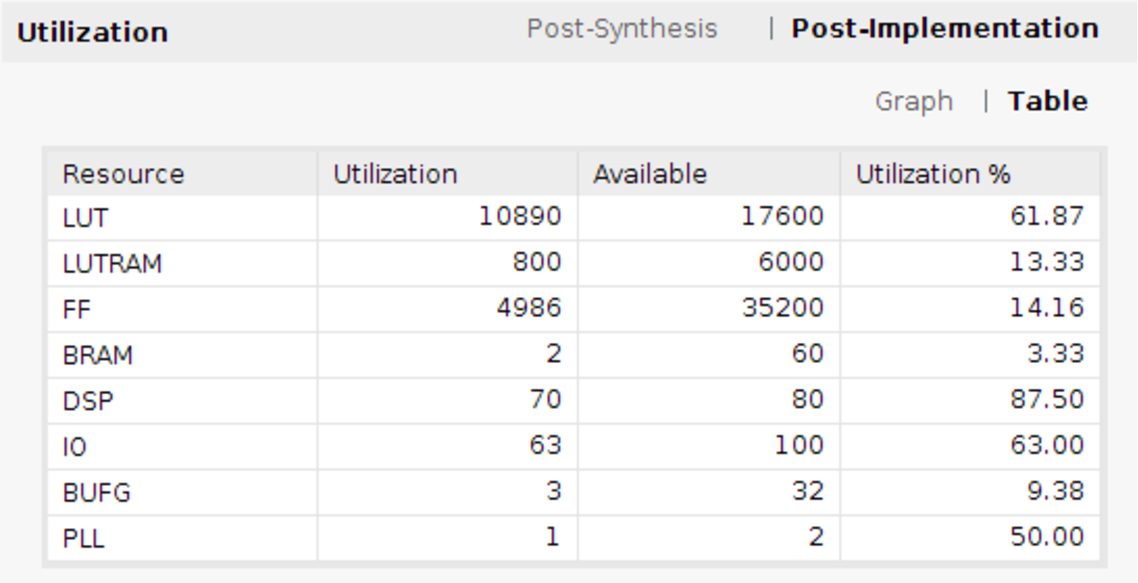
\includegraphics[width=\textwidth]{reporte_vivado_fast_rxch16}
								\end{column}
				\end{columns}
				\alert{Máximo de 40 taps para los filtros polifásicos para que trabaje a
				máxima frecuencia (125 MHz en la RedPitaya)}
\end{frame}

\begin{frame}{Simulaciones y pruebas}
				\framesubtitle{Generación de tonos de prueba}

				Cada tono, $s_k$, se define como
				\begin{equation*}\label{eq:probe_signal}
								s_k[n] = I_k[n] + jQ_k[n] = A_k e^{j\left(2\pi \frac{f_k}{f_s}n +
								\theta_k \right)},\quad n = 0,1,\ldots,2^{16}-1,
				\end{equation*}
				\begin{columns}
								\begin{column}{0.4\textwidth}
												\begin{itemize}
																\item Coeficientes generados en Python 
																\item Memorias ROM para $I[n]$ y $Q[n]$
												\end{itemize}
								\end{column}
								\begin{column}{0.6\textwidth}
												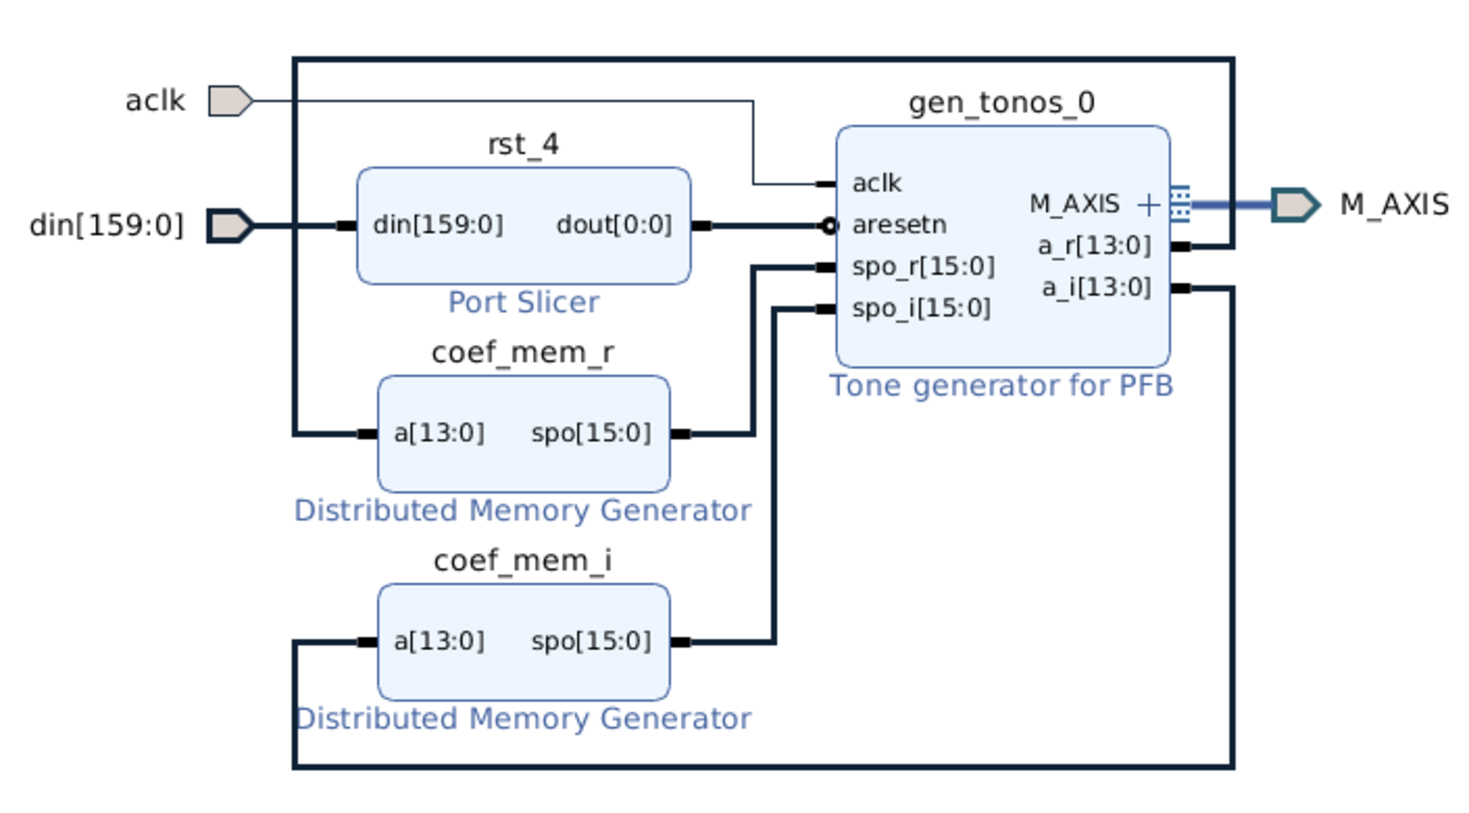
\includegraphics[width=1.2\textwidth]{gen_tonos_vivado}
								\end{column}
				\end{columns}
\end{frame}
\begin{frame}{Factor de cresta \fbox{$FC = \frac{V_p}{V_{RMS}}$}}
				\begin{columns}
								\begin{column}{0.5\textwidth}
												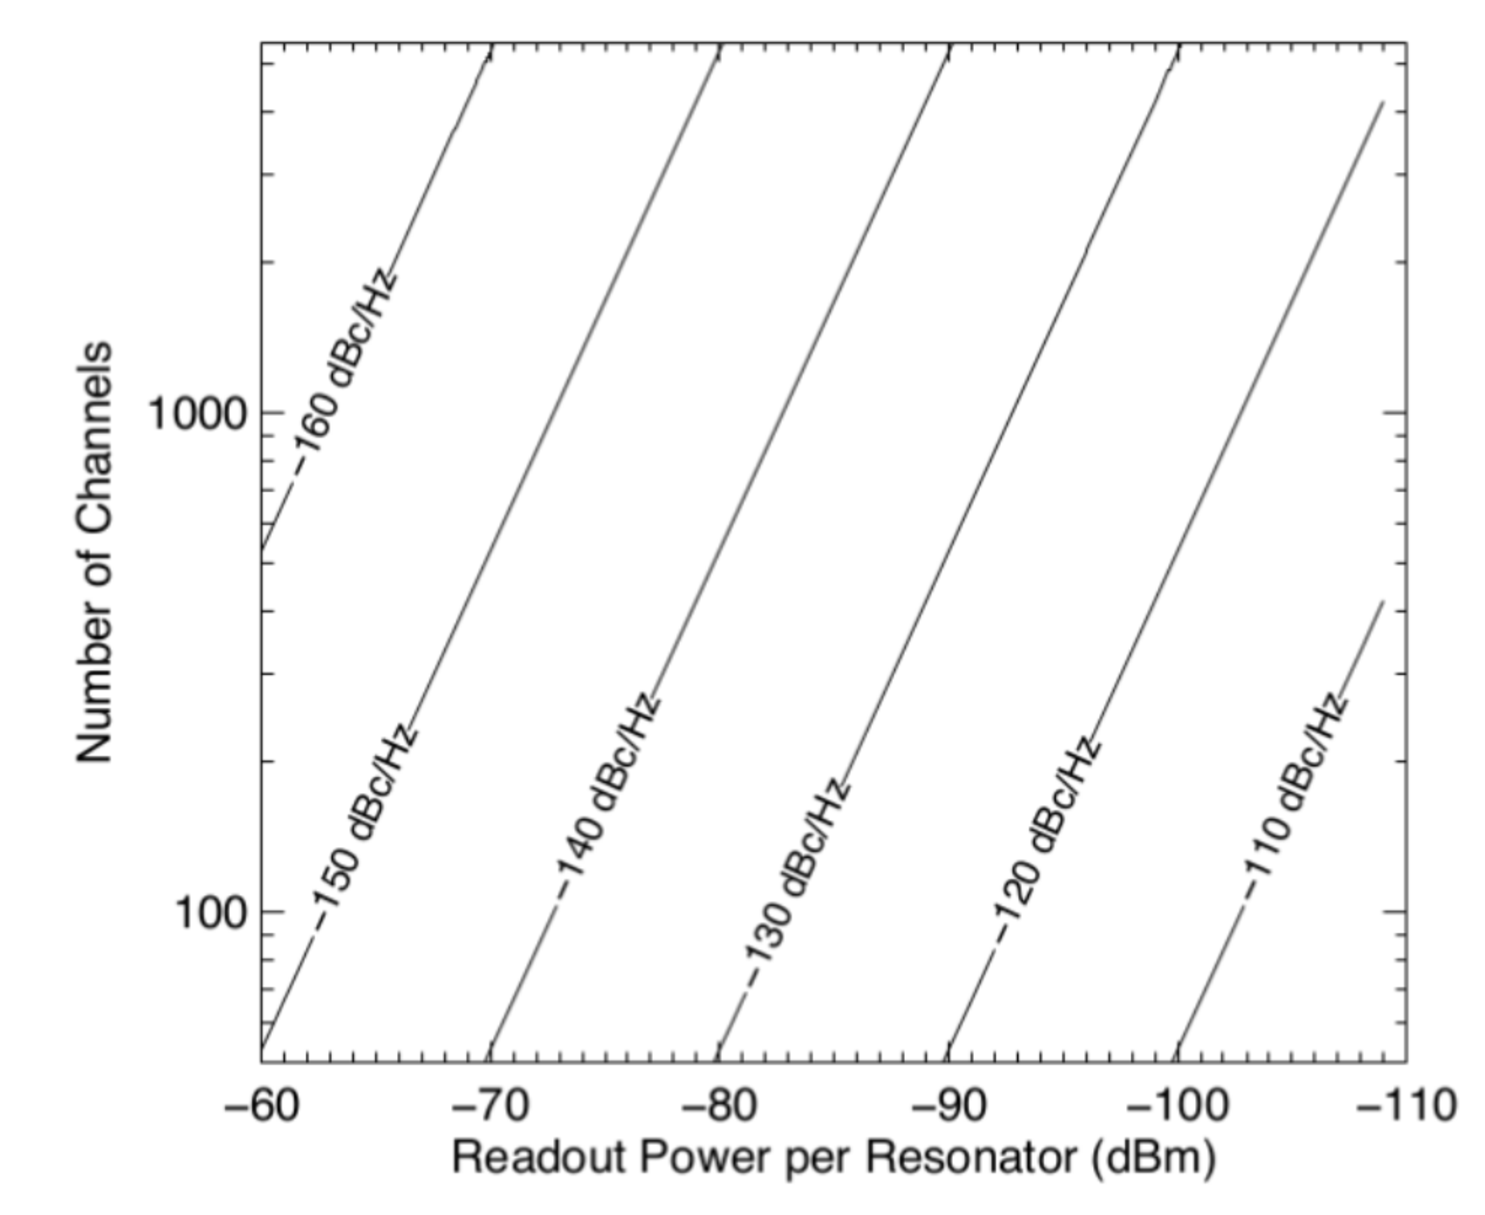
\includegraphics[width=0.7\textwidth]{power_vs_Nchannels2}
								\end{column}
								\begin{column}{0.5\textwidth}{{\color{blue}Ejemplo}}
												\footnotesize{\\(a) FC sin optimizar  : 22.627 (27.093 dB)

												(b)	FC optimizado ($A_k,\Theta_k$)  : 11.611 (21.298 dB)

												(c)	FC optimizado ($\Theta_k$)     : 8.770 (18.860 dB)

												Diferencia (a-b)                : 11.016 (5.795 dB)

												Diferencia (a-c)                : 13.857 (8.232 dB)}\\
								\end{column}
				\end{columns}
												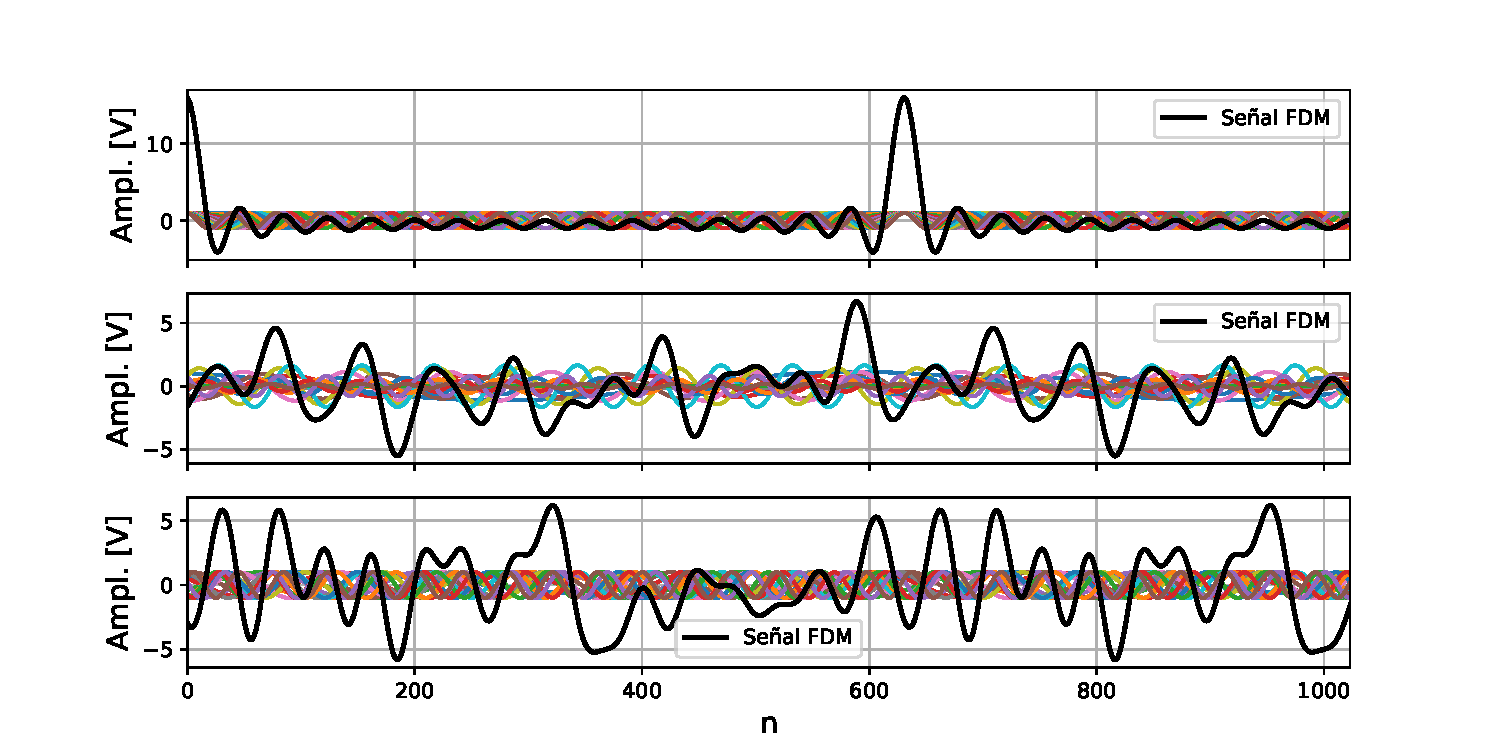
\includegraphics[width=0.85\textwidth]{in_spectrum_time2}
\end{frame}

				\begin{frame}{Simulaciones: Respuesta de los canales}
								\framesubtitle{Canales 4, 6 y 14 sin señal}
								Respuesta de simulaciones en Vivado.
								\begin{columns}
												\begin{column}{0.5\textwidth}
												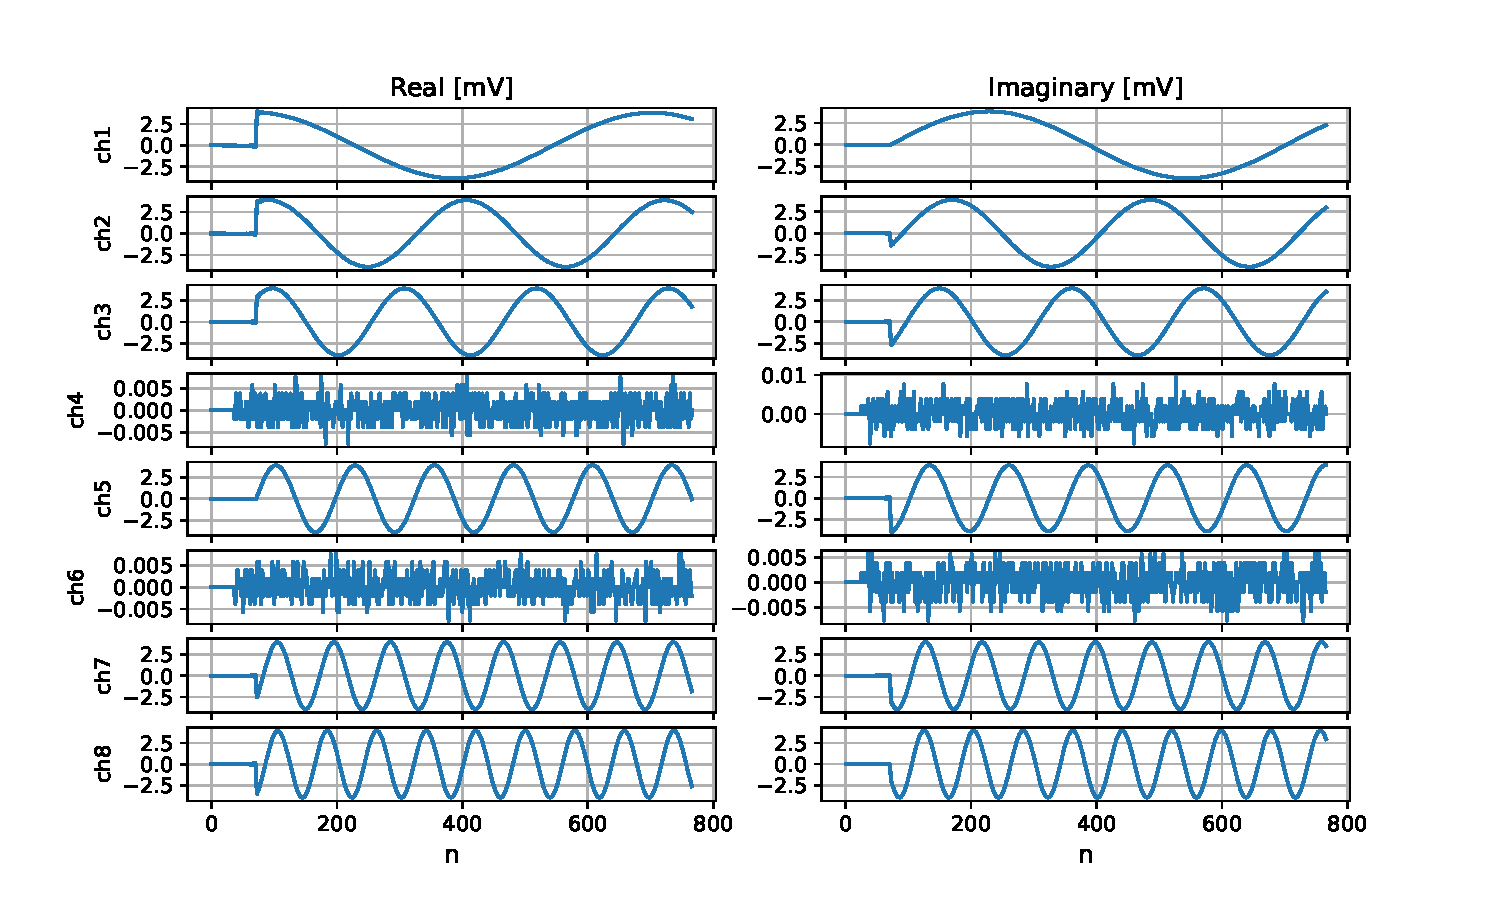
\includegraphics[width=1.2\textwidth]{gd_chann16_out_1_8}
								\end{column}
												\begin{column}{0.5\textwidth}
												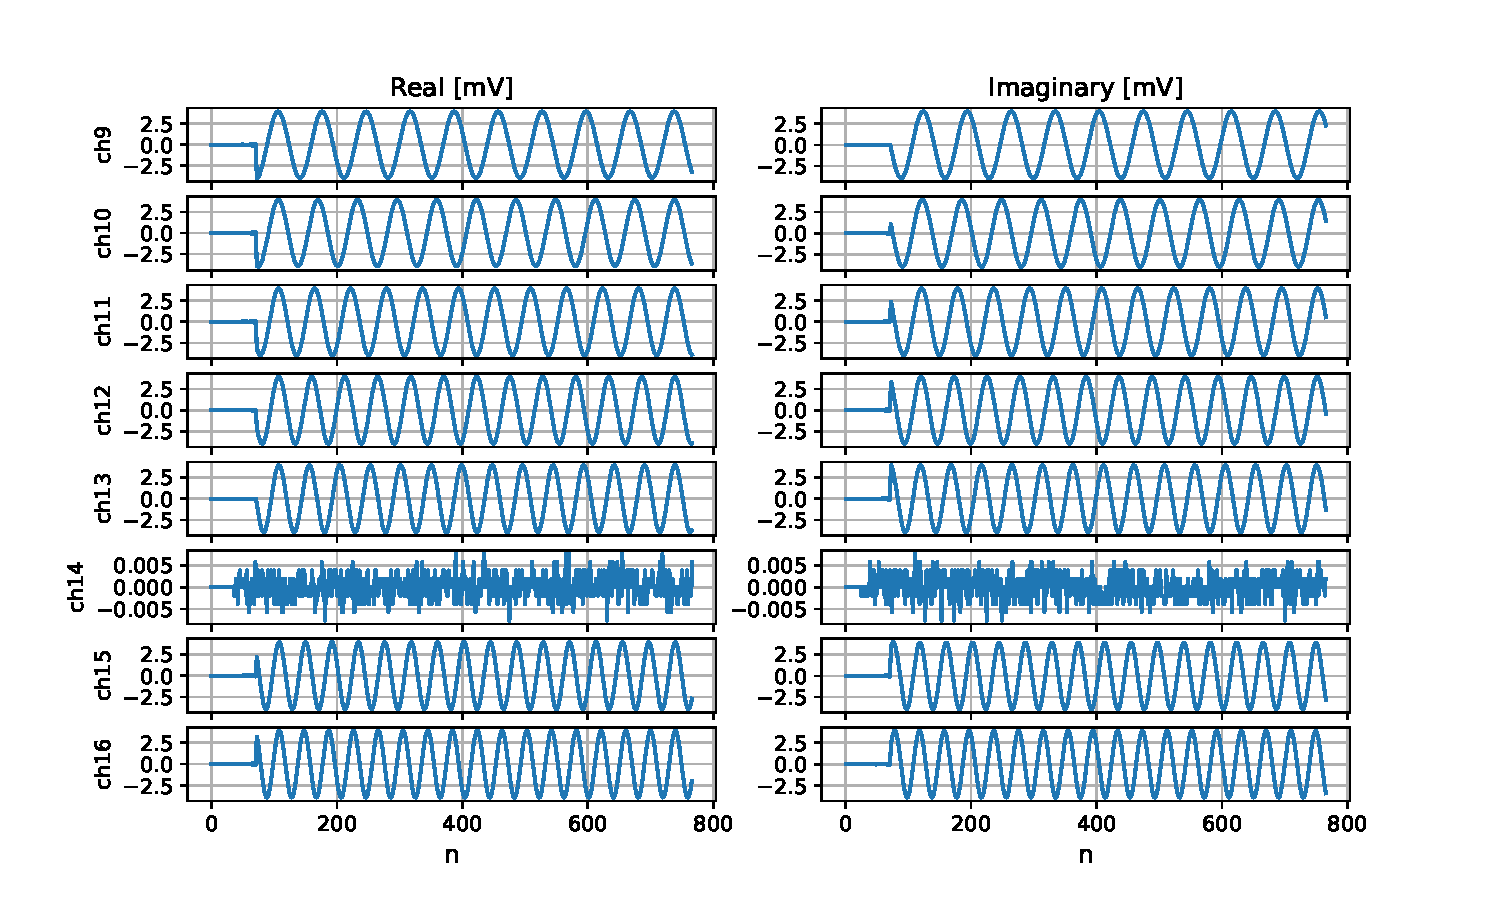
\includegraphics[width=1.2\textwidth]{gd_chann16_out_9_16}
								\end{column}
								\end{columns}
				\end{frame}

\section{Mediciones}
				\begin{frame}{Mediciones: Piso de ruido (Work in progress)}
								\framesubtitle{Canales de entrada adaptados con terminadores de
								$50\,\Omega$}
								\begin{center}
												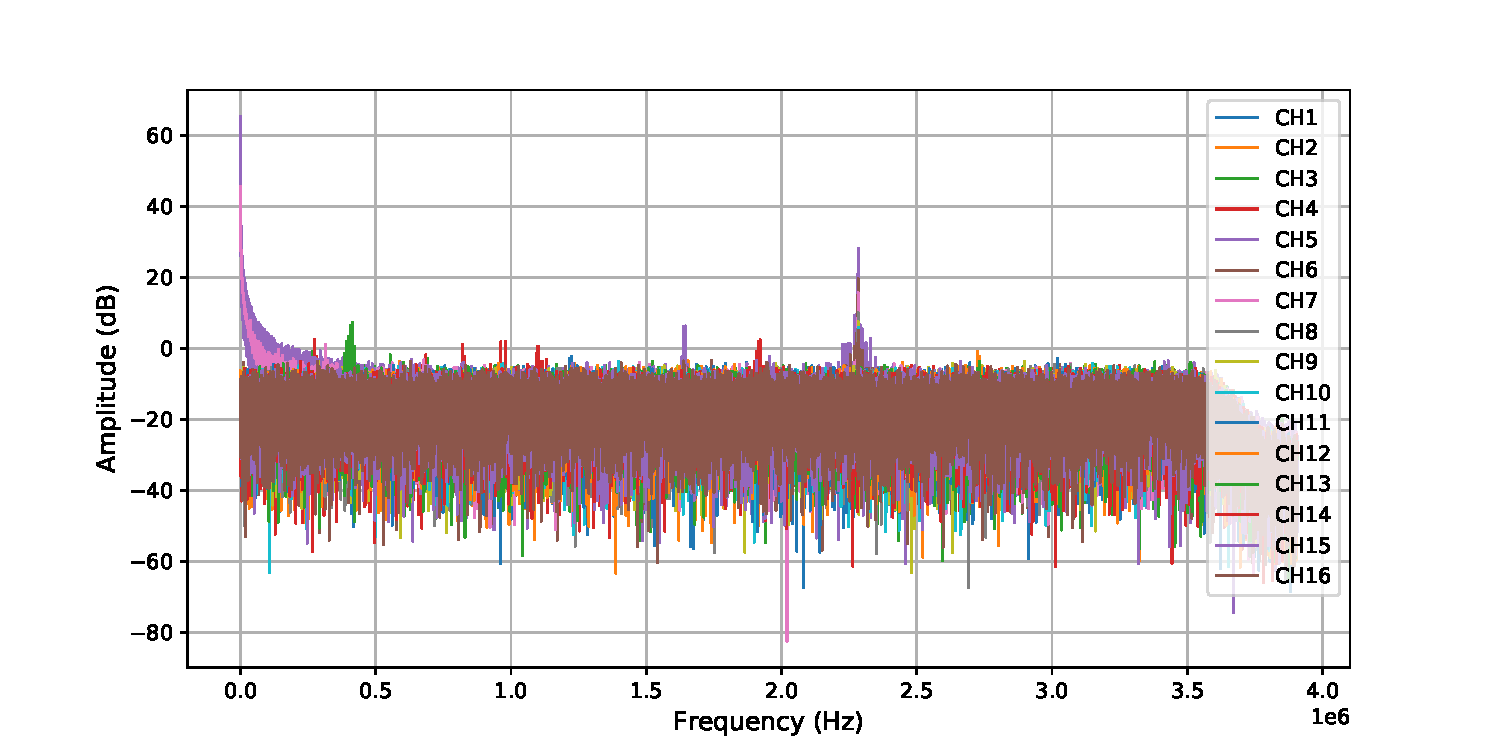
\includegraphics[width=0.56\textwidth]{noise_floor_rxch16}
								\end{center}
								\begin{columns}
												\begin{column}{0.5\textwidth}{\footnotesize{Teórico vs.
																Medido}}
																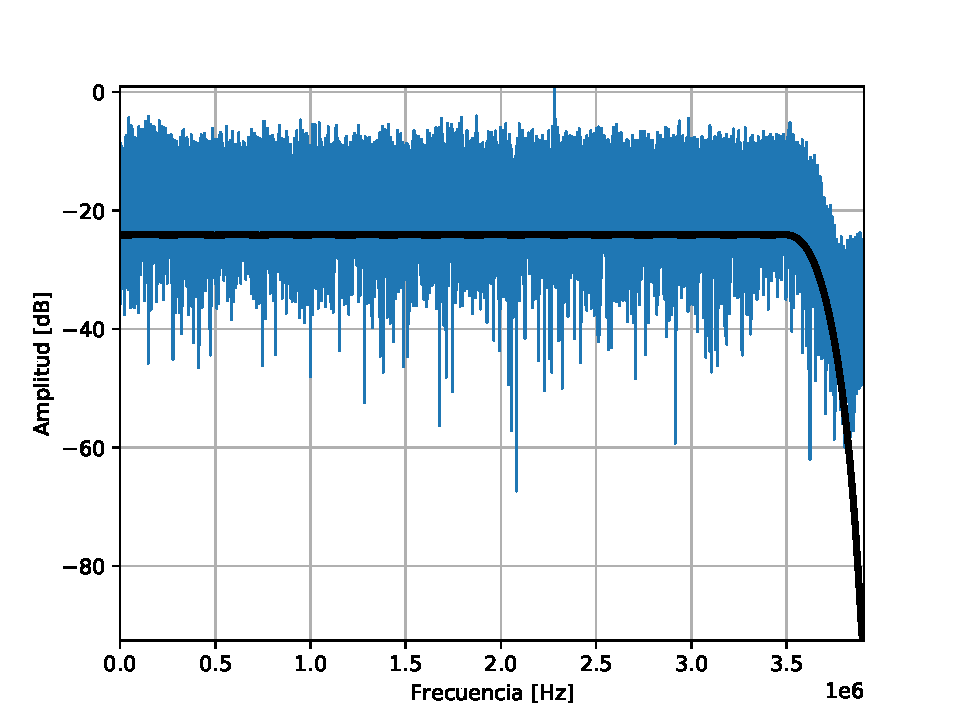
\includegraphics[width=\textwidth]{ch1}
												\end{column}
												\begin{column}{0.5\textwidth}{\footnotesize{Diferencia
																$\to$ +7dB}}
																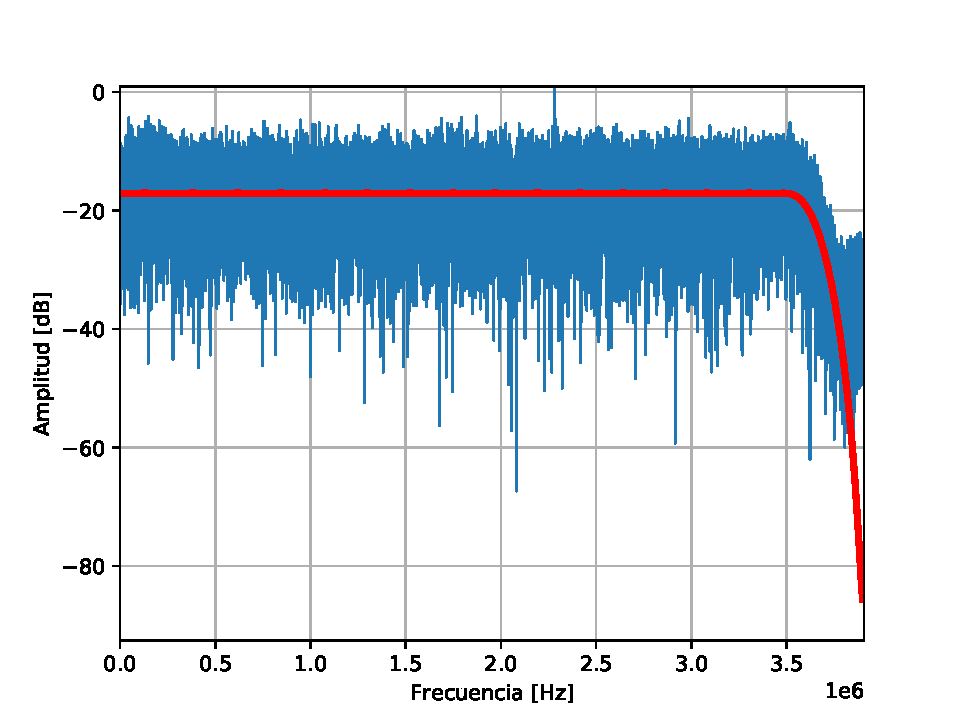
\includegraphics[width=\textwidth]{ch1_plus7dB}
												\end{column}
								\end{columns}
				\end{frame}

				\begin{frame}{Mediciones: Tonos de prueba (Work in progress)}
								\begin{center}
												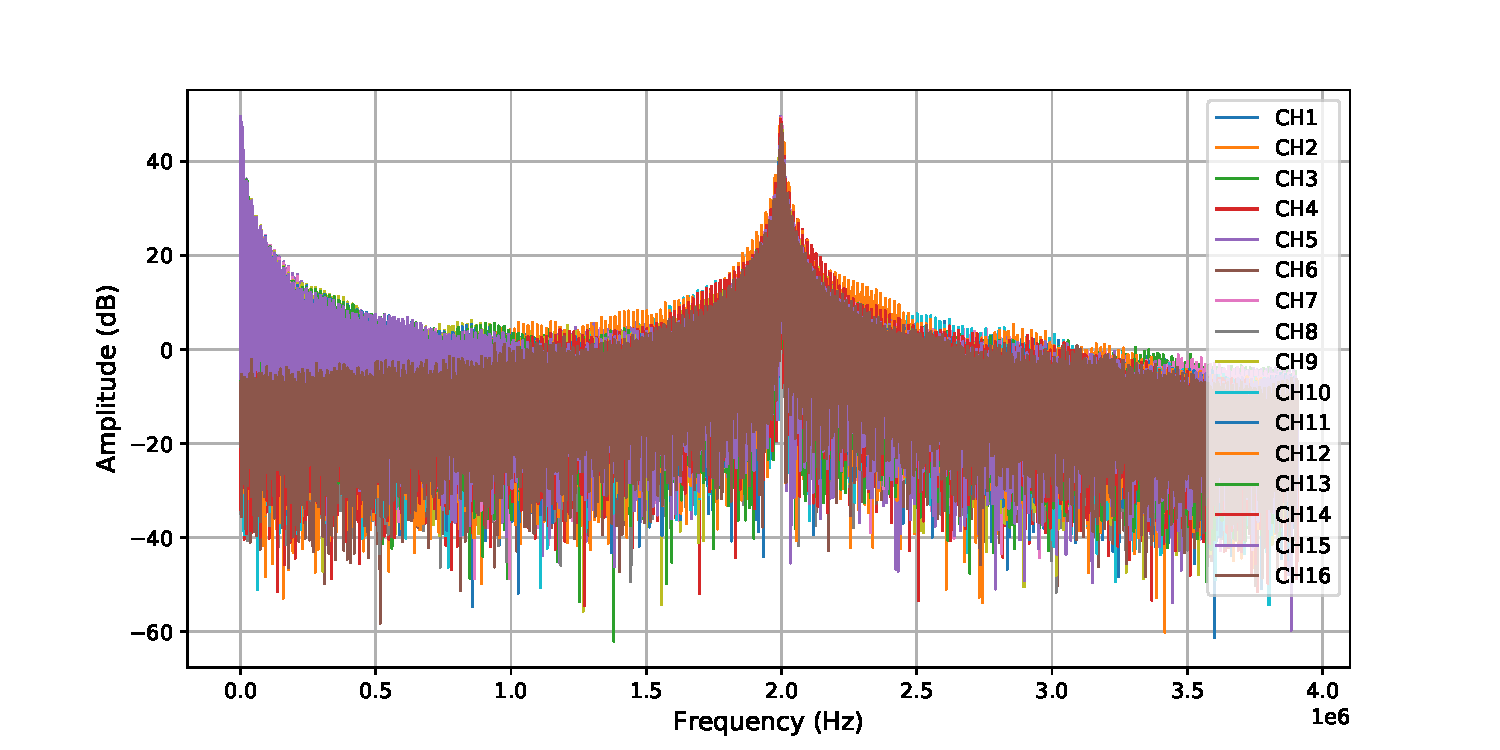
\includegraphics[width=0.7\textwidth]{fdm_out_ch16_2mhz}
												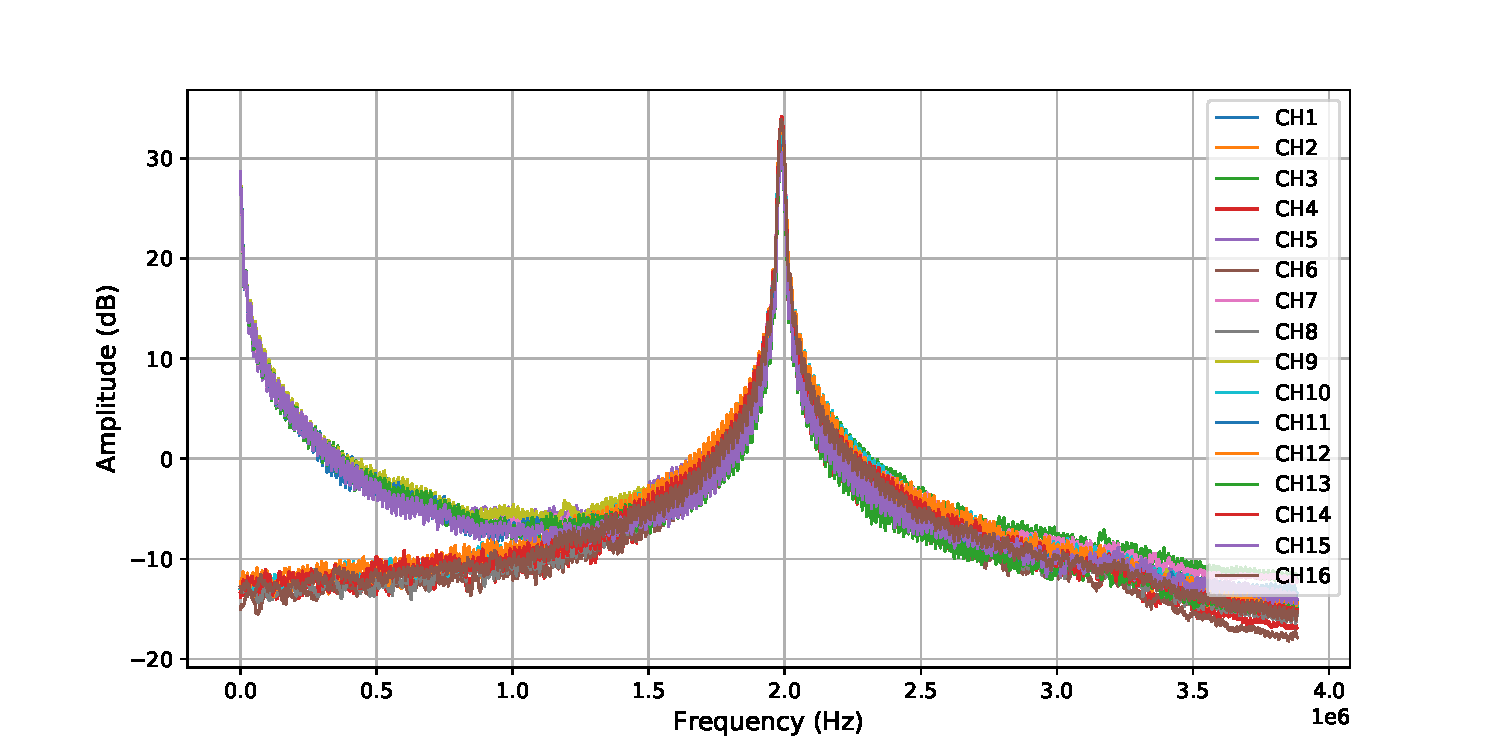
\includegraphics[width=0.7\textwidth]{ma_fdm_out_ch16_2mhz}
								\end{center}
				\end{frame}

\section{Conclusiones}
\begin{frame}{Conclusiones}
				\begin{itemize}
								\item Primeras pruebas del algoritmo de canalización en FPGA
												$\to$	Resultados prometedores
								\item Generación de programas para comprobar algoritmos en Python
								\item Armado de la configuración experimental para la medición
												de MKIDs de uso científico
								\item Se especificaron los factores determinantes para la
												excitación y lectura de los detectores superconductores MKIDs
												%\item Caracterización de MKIDs de uso científico
				\end{itemize}
\end{frame}
\section{Trabajo futuro}
\begin{frame}{Trabajo futuro}
				\begin{itemize}
												%\item Dise\~no de resonador en Sonnet
												%\item Primeras mediciones a $T_{amb}$ y $T \sim 100\,mK$
								\item Definici\'on de requerimientos para crio (cables,
												conectores, espacios, etc.)
								\item Primeras pruebas con canalizador en Bariloche (pruebas de
												front-end, mezcladores, filtros, DC-block, etc.)
								\item Pruebas con el algoritmo de Goertzel para detección de
												tonos dentro de los canales
				\end{itemize}
\end{frame}
\end{document}

